% Options for packages loaded elsewhere
\PassOptionsToPackage{unicode}{hyperref}
\PassOptionsToPackage{hyphens}{url}
%
\documentclass[
]{book}
\usepackage{lmodern}
\usepackage{amssymb,amsmath}
\usepackage{ifxetex,ifluatex}
\ifnum 0\ifxetex 1\fi\ifluatex 1\fi=0 % if pdftex
  \usepackage[T1]{fontenc}
  \usepackage[utf8]{inputenc}
  \usepackage{textcomp} % provide euro and other symbols
\else % if luatex or xetex
  \usepackage{unicode-math}
  \defaultfontfeatures{Scale=MatchLowercase}
  \defaultfontfeatures[\rmfamily]{Ligatures=TeX,Scale=1}
\fi
% Use upquote if available, for straight quotes in verbatim environments
\IfFileExists{upquote.sty}{\usepackage{upquote}}{}
\IfFileExists{microtype.sty}{% use microtype if available
  \usepackage[]{microtype}
  \UseMicrotypeSet[protrusion]{basicmath} % disable protrusion for tt fonts
}{}
\makeatletter
\@ifundefined{KOMAClassName}{% if non-KOMA class
  \IfFileExists{parskip.sty}{%
    \usepackage{parskip}
  }{% else
    \setlength{\parindent}{0pt}
    \setlength{\parskip}{6pt plus 2pt minus 1pt}}
}{% if KOMA class
  \KOMAoptions{parskip=half}}
\makeatother
\usepackage{xcolor}
\IfFileExists{xurl.sty}{\usepackage{xurl}}{} % add URL line breaks if available
\IfFileExists{bookmark.sty}{\usepackage{bookmark}}{\usepackage{hyperref}}
\hypersetup{
  pdftitle={Data Science Research Circle},
  pdfauthor={Pomona College Data Science Research Circle},
  hidelinks,
  pdfcreator={LaTeX via pandoc}}
\urlstyle{same} % disable monospaced font for URLs
\usepackage{color}
\usepackage{fancyvrb}
\newcommand{\VerbBar}{|}
\newcommand{\VERB}{\Verb[commandchars=\\\{\}]}
\DefineVerbatimEnvironment{Highlighting}{Verbatim}{commandchars=\\\{\}}
% Add ',fontsize=\small' for more characters per line
\usepackage{framed}
\definecolor{shadecolor}{RGB}{248,248,248}
\newenvironment{Shaded}{\begin{snugshade}}{\end{snugshade}}
\newcommand{\AlertTok}[1]{\textcolor[rgb]{0.94,0.16,0.16}{#1}}
\newcommand{\AnnotationTok}[1]{\textcolor[rgb]{0.56,0.35,0.01}{\textbf{\textit{#1}}}}
\newcommand{\AttributeTok}[1]{\textcolor[rgb]{0.77,0.63,0.00}{#1}}
\newcommand{\BaseNTok}[1]{\textcolor[rgb]{0.00,0.00,0.81}{#1}}
\newcommand{\BuiltInTok}[1]{#1}
\newcommand{\CharTok}[1]{\textcolor[rgb]{0.31,0.60,0.02}{#1}}
\newcommand{\CommentTok}[1]{\textcolor[rgb]{0.56,0.35,0.01}{\textit{#1}}}
\newcommand{\CommentVarTok}[1]{\textcolor[rgb]{0.56,0.35,0.01}{\textbf{\textit{#1}}}}
\newcommand{\ConstantTok}[1]{\textcolor[rgb]{0.00,0.00,0.00}{#1}}
\newcommand{\ControlFlowTok}[1]{\textcolor[rgb]{0.13,0.29,0.53}{\textbf{#1}}}
\newcommand{\DataTypeTok}[1]{\textcolor[rgb]{0.13,0.29,0.53}{#1}}
\newcommand{\DecValTok}[1]{\textcolor[rgb]{0.00,0.00,0.81}{#1}}
\newcommand{\DocumentationTok}[1]{\textcolor[rgb]{0.56,0.35,0.01}{\textbf{\textit{#1}}}}
\newcommand{\ErrorTok}[1]{\textcolor[rgb]{0.64,0.00,0.00}{\textbf{#1}}}
\newcommand{\ExtensionTok}[1]{#1}
\newcommand{\FloatTok}[1]{\textcolor[rgb]{0.00,0.00,0.81}{#1}}
\newcommand{\FunctionTok}[1]{\textcolor[rgb]{0.00,0.00,0.00}{#1}}
\newcommand{\ImportTok}[1]{#1}
\newcommand{\InformationTok}[1]{\textcolor[rgb]{0.56,0.35,0.01}{\textbf{\textit{#1}}}}
\newcommand{\KeywordTok}[1]{\textcolor[rgb]{0.13,0.29,0.53}{\textbf{#1}}}
\newcommand{\NormalTok}[1]{#1}
\newcommand{\OperatorTok}[1]{\textcolor[rgb]{0.81,0.36,0.00}{\textbf{#1}}}
\newcommand{\OtherTok}[1]{\textcolor[rgb]{0.56,0.35,0.01}{#1}}
\newcommand{\PreprocessorTok}[1]{\textcolor[rgb]{0.56,0.35,0.01}{\textit{#1}}}
\newcommand{\RegionMarkerTok}[1]{#1}
\newcommand{\SpecialCharTok}[1]{\textcolor[rgb]{0.00,0.00,0.00}{#1}}
\newcommand{\SpecialStringTok}[1]{\textcolor[rgb]{0.31,0.60,0.02}{#1}}
\newcommand{\StringTok}[1]{\textcolor[rgb]{0.31,0.60,0.02}{#1}}
\newcommand{\VariableTok}[1]{\textcolor[rgb]{0.00,0.00,0.00}{#1}}
\newcommand{\VerbatimStringTok}[1]{\textcolor[rgb]{0.31,0.60,0.02}{#1}}
\newcommand{\WarningTok}[1]{\textcolor[rgb]{0.56,0.35,0.01}{\textbf{\textit{#1}}}}
\usepackage{longtable,booktabs}
% Correct order of tables after \paragraph or \subparagraph
\usepackage{etoolbox}
\makeatletter
\patchcmd\longtable{\par}{\if@noskipsec\mbox{}\fi\par}{}{}
\makeatother
% Allow footnotes in longtable head/foot
\IfFileExists{footnotehyper.sty}{\usepackage{footnotehyper}}{\usepackage{footnote}}
\makesavenoteenv{longtable}
\usepackage{graphicx,grffile}
\makeatletter
\def\maxwidth{\ifdim\Gin@nat@width>\linewidth\linewidth\else\Gin@nat@width\fi}
\def\maxheight{\ifdim\Gin@nat@height>\textheight\textheight\else\Gin@nat@height\fi}
\makeatother
% Scale images if necessary, so that they will not overflow the page
% margins by default, and it is still possible to overwrite the defaults
% using explicit options in \includegraphics[width, height, ...]{}
\setkeys{Gin}{width=\maxwidth,height=\maxheight,keepaspectratio}
% Set default figure placement to htbp
\makeatletter
\def\fps@figure{htbp}
\makeatother
\setlength{\emergencystretch}{3em} % prevent overfull lines
\providecommand{\tightlist}{%
  \setlength{\itemsep}{0pt}\setlength{\parskip}{0pt}}
\setcounter{secnumdepth}{5}
\usepackage{booktabs}
\usepackage{amsthm}
\makeatletter
\def\thm@space@setup{%
  \thm@preskip=8pt plus 2pt minus 4pt
  \thm@postskip=\thm@preskip
}
\makeatother
\usepackage[]{natbib}
\bibliographystyle{apalike}

\title{Data Science Research Circle}
\author{Pomona College Data Science Research Circle}
\date{2020-05-29}

\begin{document}
\maketitle

{
\setcounter{tocdepth}{1}
\tableofcontents
}
\hypertarget{preface}{%
\chapter{Preface}\label{preface}}

\quad Welcome! This page is the manifestation of a semester-long investigative project conducted by a Data Science Research Circle at Pomona College in Claremont, CA. The research circle consisted of seven students including: \href{https://github.com/Amber-Patricia-Lee}{Amber Lee} (`22), \href{https://github.com/armwong9}{Arm Wonghirundacha} (`22), \href{https://github.com/emmacgodfrey}{Emma Godfrey} (`21), \href{https://github.com/eruong}{Ethan Ong} (`21), \href{https://github.com/iyyuan1208}{Ivy Yuan} (`21), \href{https://github.com/oliverc1623}{Oliver Chang} (`22), and \href{https://github.com/wega2018}{Will Gray} (`22). Additionally the research circle was advised by Professors \href{https://research.pomona.edu/johardin/}{Jo Hardin} and \href{https://www.pomona.edu/directory/people/ghassan-y-sarkis}{Ghassan Sarkis} from the Department of Mathematics. The work is motivated by recent literature and investigative analysis on policing practices around the country, particularly from the \href{https://openpolicing.stanford.edu/}{Stanford Open Policing Project}.

\quad The Stanford Open Policing Project is an ongoing research effort to gather and publish police stop data from around the United States. The project is a collaboration between the Stanford Computational Journalism Lab and the Stanford School of Engineering led by professor Cheryl Phillips and Sharad Goel. Beginning in 2015, the Stanford Open Policing project has requested both state-wide and city-wide public information about police stops; requests were filed for all 50 states and over 100 cities. On June 19th 2017, the project published the collected data on their website openpolicing.stanford.edu and as of 2020, the website holds data from 42 states totalling 255 million data points. 221 million of these stops were from 33 state patrol datasets collected and the remaining 34 million were from 56 city-wide datasets.

\quad One of the primary focuses of the Stanford Open Policing Project is traffic stop data. More than 50,000 traffic stops occur every day --- 20 million in a year --- yet prior to the debut of the Open Policing Project database, there was a lack of reliable, comprehensive, and standardized national datasets on these traffic stop data to analyze. The Open Policing Project provides a unique opportunity to investigate these traffic stops, with particular intention to work towards a definitive test of racial profiling. The interdisciplinary work towards developing a definitive test of racial profiling is grounded in social and political relevance -- the true extent of racial profiling would be crucial tool for informing police department trainings, protecting Fourth Amendment rights of minority defendants, and validating the qualitative experiences of historically-oppressed groups (Goel 2017).

\quad The motivation for this project is to continue the analysis of the Stanford Open Policing Project dataset. This includes reproducing previous findings and applying methodologies used on smaller datasets to the Stanford nation-wide database. The three topics of interest before beginning EDA for this project were the following: the enactment of seatbelt laws and its effect on traffic stops, night versus day stops, and discrepancies of search rates. Not all were pursued, but each provided a unique direction for data analysis. The report is organized into several parts: I. Preface, II. Literature Review, III. Description of Data, IV. Databases/Using SQL, V. Exploratory Data Analysis, and VI. Limitations and Discussion.

\hypertarget{functions}{%
\chapter{Functions}\label{functions}}

This section explains the various functions used throughout our research.

\hypertarget{data-uploading-functions}{%
\section{Data Uploading Functions}\label{data-uploading-functions}}

The functions here serve as cleaning functions such that a ready to use dataset gets uploaded to the database as a data table.

convertLogicalToInt function:
input: dataset
output: dataset with logical values set to binary

\begin{Shaded}
\begin{Highlighting}[]
\NormalTok{convertLogicalToInt <-}\StringTok{ }\ControlFlowTok{function}\NormalTok{(input_df)\{}
\NormalTok{  vars <-}\StringTok{ }\KeywordTok{sapply}\NormalTok{(input_df, class) }\OperatorTok\StringTok{ }
\StringTok{  }\KeywordTok{list.which}\NormalTok{(.}\OperatorTok{==}\StringTok{'logical'}\NormalTok{)}

\NormalTok{  input_df[,vars] <-}\StringTok{ }\KeywordTok{sapply}\NormalTok{(input_df[,vars], as.numeric)}
\NormalTok{  input_df}
  \KeywordTok{return}\NormalTok{(input_df)}
\NormalTok{\}}
\end{Highlighting}
\end{Shaded}

getDFName:
input: name of dataset (this could also be name of link from web scrape)
output: clean dataset name that includes state and city

\begin{Shaded}
\begin{Highlighting}[]
\NormalTok{getDFName <-}\StringTok{ }\ControlFlowTok{function}\NormalTok{(input_string)\{}
\NormalTok{  tmp <-}\StringTok{ }\KeywordTok{str_split}\NormalTok{(input_string, }\StringTok{'_'}\NormalTok{, }\DataTypeTok{simplify =} \OtherTok{TRUE}\NormalTok{)}
\NormalTok{  tmp}
  
\NormalTok{  state <-}\StringTok{ }\KeywordTok{str_to_upper}\NormalTok{(tmp[,}\DecValTok{2}\NormalTok{])}
  
  \ControlFlowTok{if}\NormalTok{(tmp[,}\DecValTok{4}\NormalTok{] }\OperatorTok{!=}\StringTok{ "2019"}\NormalTok{)\{}
\NormalTok{      cityName <-}\StringTok{ }\KeywordTok{paste}\NormalTok{(tmp[,}\DecValTok{3}\NormalTok{], tmp[,}\DecValTok{4}\NormalTok{], }\DataTypeTok{sep=}\StringTok{""}\NormalTok{)}
\NormalTok{      name <-}\StringTok{ }\KeywordTok{paste}\NormalTok{(state, cityName, }\DataTypeTok{sep=}\StringTok{""}\NormalTok{)}
\NormalTok{  \} }\ControlFlowTok{else}\NormalTok{ \{}
\NormalTok{      cityName <-}\StringTok{ }\NormalTok{tmp[,}\DecValTok{3}\NormalTok{]}
\NormalTok{      name <-}\StringTok{ }\KeywordTok{paste}\NormalTok{(state, cityName, }\DataTypeTok{sep=}\StringTok{""}\NormalTok{)}
\NormalTok{  \}}
\NormalTok{  name}
  \KeywordTok{return}\NormalTok{(name)}
\NormalTok{\}}
\end{Highlighting}
\end{Shaded}

uploadLinksToDatabase:
input: string link from web scrape
outout: 0 - indicating that the code finished executing
This function will take in a RDS link and write the dataset to the database

\begin{Shaded}
\begin{Highlighting}[]
\NormalTok{uploadLinksToDatabase <-}\StringTok{ }\ControlFlowTok{function}\NormalTok{(input_link)\{}
\NormalTok{  tmpDF <-}\StringTok{ }\KeywordTok{readRDS}\NormalTok{(}\KeywordTok{gzcon}\NormalTok{(}\KeywordTok{url}\NormalTok{(input_link)))}
\NormalTok{  tmpDF <-}\StringTok{ }\KeywordTok{convertLogicalToInt}\NormalTok{(tmpDF)}
\NormalTok{  name<-}\StringTok{ }\KeywordTok{getDFName}\NormalTok{(input_link)}
  
  \KeywordTok{dbWriteTable}\NormalTok{(con2, name, tmpDF, }\DataTypeTok{overwrite =} \OtherTok{TRUE}\NormalTok{)}
  \KeywordTok{return}\NormalTok{(}\DecValTok{0}\NormalTok{)}
\NormalTok{\}}
\end{Highlighting}
\end{Shaded}

\hypertarget{veil-of-darkness-functions}{%
\section{Veil of Darkness Functions}\label{veil-of-darkness-functions}}

Veil of Darkness functions work with lutz and lubridate to determine whether a stop took place in the dark.

The first step in getting the sunset and sunrise times is to get the coordinates for the city. To do this, we can Google search the city name and webscrape the Google search results.

The two code chunk below has functions that will perform this process. get\_cityNames takes in a datatable's name and cleans it so that the google search engine result will return the desired page that has the coordinates.

\begin{Shaded}
\begin{Highlighting}[]
\NormalTok{get_cityNames <-}\StringTok{ }\ControlFlowTok{function}\NormalTok{(name)\{}
\NormalTok{  check <-}\StringTok{ }\KeywordTok{str_extract}\NormalTok{(name, }\StringTok{"[a-z]+"}\NormalTok{)}
  \ControlFlowTok{if}\NormalTok{(check }\OperatorTok{==}\StringTok{ "statewide"}\NormalTok{)\{}
    \KeywordTok{return}\NormalTok{(state.name[}\KeywordTok{grep}\NormalTok{(}\KeywordTok{str_sub}\NormalTok{(name, }\DecValTok{1}\NormalTok{,}\DecValTok{2}\NormalTok{), state.abb)])}
\NormalTok{  \} }\ControlFlowTok{else}\NormalTok{ \{}
    \KeywordTok{return}\NormalTok{(check)}
\NormalTok{  \}}
\NormalTok{\}}
\end{Highlighting}
\end{Shaded}

get\_coordinates takes in said clean city names and scrape the google search web result. The function will return a vector of doubles. The first index is for latitude and second index has longitude.

\begin{Shaded}
\begin{Highlighting}[]
\NormalTok{get_coordinates <-}\StringTok{ }\ControlFlowTok{function}\NormalTok{(city)\{}
\NormalTok{  url <-}\StringTok{ }
\StringTok{    }\KeywordTok{paste}\NormalTok{(}\StringTok{"https://www.google.com/search?q="}\NormalTok{,}
\NormalTok{          city,}
          \StringTok{"+lat+long&oq=sandiego+lat+long&aqs=chrome..69i57.2463j0j7&sourceid=chrome&ie=UTF-8"}\NormalTok{)}
\NormalTok{  doc <-}\StringTok{ }\KeywordTok{htmlParse}\NormalTok{(}\KeywordTok{readLines}\NormalTok{(url), }\DataTypeTok{asText=}\OtherTok{TRUE}\NormalTok{)}
\NormalTok{  links <-}\StringTok{ }\KeywordTok{xpathSApply}\NormalTok{(doc, }\StringTok{"//div[@class='kCrYT']"}\NormalTok{, xmlValue)}
\NormalTok{  clean_coor <-}\StringTok{ }\KeywordTok{as.list}\NormalTok{(}\KeywordTok{str_split}\NormalTok{(links[}\DecValTok{2}\NormalTok{], }\StringTok{","}\NormalTok{))}
\NormalTok{  lat <-}\StringTok{ }\KeywordTok{as.numeric}\NormalTok{(}\KeywordTok{str_extract}\NormalTok{(clean_coor[[}\DecValTok{1}\NormalTok{]][}\DecValTok{1}\NormalTok{], }\StringTok{"}\CharTok{\textbackslash{}\textbackslash{}}\StringTok{d+}\CharTok{\textbackslash{}\textbackslash{}}\StringTok{.*}\CharTok{\textbackslash{}\textbackslash{}}\StringTok{d*"}\NormalTok{))}
\NormalTok{  long <-}\StringTok{ }\DecValTok{-1}\OperatorTok{*}\KeywordTok{as.numeric}\NormalTok{(}\KeywordTok{str_extract}\NormalTok{(clean_coor[[}\DecValTok{1}\NormalTok{]][}\DecValTok{2}\NormalTok{], }\StringTok{"}\CharTok{\textbackslash{}\textbackslash{}}\StringTok{d+}\CharTok{\textbackslash{}\textbackslash{}}\StringTok{.*}\CharTok{\textbackslash{}\textbackslash{}}\StringTok{d*"}\NormalTok{))}
\NormalTok{  x <-}\StringTok{ }\KeywordTok{c}\NormalTok{(lat,long)}
  \KeywordTok{return}\NormalTok{(x)}
\NormalTok{\}}

\NormalTok{clean_names <-}\StringTok{ }\KeywordTok{list}\NormalTok{()}
\NormalTok{clean_names <-}\StringTok{ }\KeywordTok{lapply}\NormalTok{(datasets_of_interest, get_cityNames)}
\NormalTok{coordinates <-}\StringTok{ }\KeywordTok{lapply}\NormalTok{(clean_names,get_coordinates)}
\end{Highlighting}
\end{Shaded}

Next, we will define two helper functions in getting that call the lutz package and retrieve the times.

outsunriseset
input: latitude (dbl), longitude(dbl), date(Date or Posix), timezime (tz), direction(string)
output: Date with time of the desired sun direction

\begin{Shaded}
\begin{Highlighting}[]
\NormalTok{oursunriseset <-}\StringTok{ }\ControlFlowTok{function}\NormalTok{(latitude, longitude, date, timezone, direction) \{}
\NormalTok{  date.lat.long <-}\StringTok{ }\KeywordTok{data.frame}\NormalTok{(}\DataTypeTok{date =}\NormalTok{ date, }\DataTypeTok{lat =}\NormalTok{ latitude, }\DataTypeTok{lon =}\NormalTok{ longitude)}
  \ControlFlowTok{if}\NormalTok{(direction }\OperatorTok{==}\StringTok{ "sunset"}\NormalTok{)\{}
    \CommentTok{# call getSunlightTimes from the lutz package}
    \KeywordTok{getSunlightTimes}\NormalTok{(}\DataTypeTok{data =}\NormalTok{ date.lat.long, }\DataTypeTok{keep=}\NormalTok{direction, }\DataTypeTok{tz=}\NormalTok{timezone)}\OperatorTok{$}\NormalTok{sunset }
\NormalTok{  \} }\ControlFlowTok{else} \ControlFlowTok{if}\NormalTok{(direction }\OperatorTok{==}\StringTok{ "sunrise"}\NormalTok{)\{}
    \KeywordTok{getSunlightTimes}\NormalTok{(}\DataTypeTok{data =}\NormalTok{ date.lat.long, }\DataTypeTok{keep=}\NormalTok{direction, }\DataTypeTok{tz=}\NormalTok{timezone)}\OperatorTok{$}\NormalTok{sunrise  }
\NormalTok{  \} }\ControlFlowTok{else} \ControlFlowTok{if}\NormalTok{ (direction }\OperatorTok{==}\StringTok{ "dusk"}\NormalTok{)\{}
    \KeywordTok{getSunlightTimes}\NormalTok{(}\DataTypeTok{data =}\NormalTok{ date.lat.long, }\DataTypeTok{keep=}\NormalTok{direction, }\DataTypeTok{tz=}\NormalTok{timezone)}\OperatorTok{$}\NormalTok{dusk}
\NormalTok{  \} }\ControlFlowTok{else} \ControlFlowTok{if}\NormalTok{ (direction }\OperatorTok{==}\StringTok{ "dawn"}\NormalTok{)\{}
    \KeywordTok{getSunlightTimes}\NormalTok{(}\DataTypeTok{data =}\NormalTok{ date.lat.long, }\DataTypeTok{keep=}\NormalTok{direction, }\DataTypeTok{tz=}\NormalTok{timezone)}\OperatorTok{$}\NormalTok{dawn}
\NormalTok{  \}}
\NormalTok{\}}
\end{Highlighting}
\end{Shaded}

time\_to\_minute is the helper function the Stanford Open Policing Project uses in their tutorial to help convert times into a numeric values that's easier to manipulate - this will be useful when splicing out times between sunset and dusk to remove ambiguouity in the intertwilight zone.
input: time (character)
output: minutes (double)

\begin{Shaded}
\begin{Highlighting}[]
\NormalTok{time_to_minute <-}\StringTok{ }\ControlFlowTok{function}\NormalTok{(time) \{}
  \KeywordTok{hour}\NormalTok{(}\KeywordTok{hms}\NormalTok{(time)) }\OperatorTok{*}\StringTok{ }\DecValTok{60} \OperatorTok{+}\StringTok{ }\KeywordTok{minute}\NormalTok{(}\KeywordTok{hms}\NormalTok{(time))}
\NormalTok{\}}
\end{Highlighting}
\end{Shaded}

add\_night\_day function utilizes oursunriseset function to mutate sunrise and sunset times and a binary variables to see if the stop happened in the night of day. In addition, this function takes out the intertwilightzone i.e.~stops between sunset and dusk and dawn and sunrise.

\begin{Shaded}
\begin{Highlighting}[]
\NormalTok{add_night_day <-}\StringTok{ }\ControlFlowTok{function}\NormalTok{(city_df, time_zone, lat, long)\{}
    
\NormalTok{    sunset_times <-}\StringTok{ }\NormalTok{city_df }\OperatorTok\StringTok{ }\KeywordTok{distinct}\NormalTok{(date) }\OperatorTok\StringTok{ }\KeywordTok{mutate}\NormalTok{(}\DataTypeTok{date =} \KeywordTok{as.Date}\NormalTok{(}\KeywordTok{ymd}\NormalTok{(date, }\DataTypeTok{tz =}\NormalTok{ time_zone))) }\OperatorTok\StringTok{ }
\StringTok{  }\KeywordTok{mutate}\NormalTok{(}\DataTypeTok{sunset =} \KeywordTok{oursunriseset}\NormalTok{(lat, long, date, time_zone, }\DataTypeTok{direction=}\StringTok{"sunset"}\NormalTok{), }
        \DataTypeTok{dusk =} \KeywordTok{oursunriseset}\NormalTok{(lat, long, date, time_zone, }\DataTypeTok{direction=}\StringTok{"dusk"}\NormalTok{),}
        \DataTypeTok{dawn =} \KeywordTok{oursunriseset}\NormalTok{(lat, long, date, time_zone, }\DataTypeTok{direction=}\StringTok{"dawn"}\NormalTok{),}
        \DataTypeTok{sunrise =} \KeywordTok{oursunriseset}\NormalTok{(lat, long, date, time_zone, }\DataTypeTok{direction=}\StringTok{"sunrise"}\NormalTok{),}
        \DataTypeTok{sunset =} \KeywordTok{format}\NormalTok{(sunset, }\StringTok{"%H:%M:%S"}\NormalTok{),}
        \DataTypeTok{dusk =} \KeywordTok{format}\NormalTok{(dusk, }\StringTok{"%H:%M:%S"}\NormalTok{),}
        \DataTypeTok{dawn =} \KeywordTok{format}\NormalTok{(dawn, }\StringTok{"%H:%M:%S"}\NormalTok{),}
        \DataTypeTok{sunrise =} \KeywordTok{format}\NormalTok{(sunrise, }\StringTok{"%H:%M:%S"}\NormalTok{),}
        \DataTypeTok{sunset_min=}\KeywordTok{time_to_minute}\NormalTok{(sunset), }
        \DataTypeTok{dusk_min=}\KeywordTok{time_to_minute}\NormalTok{(dusk),}
        \DataTypeTok{dawn_min=}\KeywordTok{time_to_minute}\NormalTok{(dawn), }
        \DataTypeTok{sunrise_min=}\KeywordTok{time_to_minute}\NormalTok{(sunrise)) }\OperatorTok\StringTok{ }\KeywordTok{drop_na}\NormalTok{()}
  
\NormalTok{  city_df <-}\StringTok{ }\NormalTok{city_df }\OperatorTok\StringTok{ }\KeywordTok{drop_na}\NormalTok{() }\OperatorTok\StringTok{ }\KeywordTok{mutate}\NormalTok{(}\DataTypeTok{date=}\KeywordTok{as.Date}\NormalTok{(}\KeywordTok{ymd}\NormalTok{(date, }\DataTypeTok{tz =}\NormalTok{ time_zone))) }\OperatorTok
\StringTok{    }\KeywordTok{left_join}\NormalTok{(sunset_times, }\DataTypeTok{by=}\StringTok{"date"}\NormalTok{) }\OperatorTok\StringTok{ }\KeywordTok{drop_na}\NormalTok{() }\OperatorTok\StringTok{ }
\StringTok{    }\KeywordTok{mutate}\NormalTok{(}\DataTypeTok{minute =} \KeywordTok{time_to_minute}\NormalTok{(time), }
           \DataTypeTok{minutes_after_dark =}\NormalTok{ minute }\OperatorTok{-}\StringTok{ }\NormalTok{dusk_min,}
           \DataTypeTok{is_dark =} \KeywordTok{as.factor}\NormalTok{(minute }\OperatorTok{>}\StringTok{ }\NormalTok{dusk_min }\OperatorTok{|}\StringTok{ }\NormalTok{minute }\OperatorTok{<}\StringTok{ }\NormalTok{dawn_min)) }\OperatorTok\StringTok{ }
\StringTok{        }\CommentTok{# filter out amiguous time between sunset and dusk and dawn and sunrise}
\StringTok{  }\KeywordTok{filter}\NormalTok{(}\OperatorTok{!}\NormalTok{(minute }\OperatorTok{>}\StringTok{ }\NormalTok{sunset_min }\OperatorTok{&}\StringTok{ }\NormalTok{minute }\OperatorTok{<}\StringTok{ }\NormalTok{dusk_min),}
         \OperatorTok{!}\NormalTok{(minute }\OperatorTok{<}\StringTok{ }\NormalTok{sunrise_min }\OperatorTok{&}\StringTok{ }\NormalTok{minute }\OperatorTok{>}\StringTok{ }\NormalTok{dawn_min)) }\OperatorTok\StringTok{ }\KeywordTok{select}\NormalTok{(subject_race, is_dark)}
    
  \CommentTok{# select(subject_race, search_conducted, subject_age, is_dark)}
  \KeywordTok{return}\NormalTok{(city_df)}
\NormalTok{\}}
\end{Highlighting}
\end{Shaded}

\hypertarget{nationwide-functions}{%
\section{Nationwide Functions}\label{nationwide-functions}}

These are functions used when analyzing multiple datatables from the database.

relevant\_dataests:
input: - all dataset names which can be acquired through SHOW TABLES sql command
- A vector containing string of variables names we wish to disect
output: a character string of dataset names

\begin{Shaded}
\begin{Highlighting}[]
\NormalTok{relevant_datasets <-}\StringTok{ }\ControlFlowTok{function}\NormalTok{(all_dataset_names, variables_of_interest)\{}
  
  \CommentTok{# create empty vector}
\NormalTok{  datasets_of_interest <-}\StringTok{ }\KeywordTok{c}\NormalTok{()}
    
  \ControlFlowTok{for}\NormalTok{(city }\ControlFlowTok{in}\NormalTok{ all_dataset_names)\{}
    
    \CommentTok{# run only if table is not empty }
\NormalTok{    check_command =}\StringTok{ }\KeywordTok{paste}\NormalTok{(}\StringTok{"SELECT 1 FROM"}\NormalTok{, city, }\DataTypeTok{sep=}\StringTok{" "}\NormalTok{, }\StringTok{"LIMIT 1"}\NormalTok{)}
\NormalTok{    count <-}\StringTok{ }\NormalTok{DBI}\OperatorTok{::}\KeywordTok{dbGetQuery}\NormalTok{(con, check_command)}
    
    \ControlFlowTok{if}\NormalTok{(}\KeywordTok{nrow}\NormalTok{(count) }\OperatorTok{!=}\StringTok{ }\DecValTok{0}\NormalTok{)\{}
      \CommentTok{# cancenate SQL query string}
\NormalTok{      command <-}\StringTok{ }\KeywordTok{paste}\NormalTok{(}\StringTok{"EXPLAIN"}\NormalTok{, city, }\DataTypeTok{sep =} \StringTok{" "}\NormalTok{)}
\NormalTok{      field_vector <-}\StringTok{ }\KeywordTok{unlist}\NormalTok{(}\KeywordTok{as.list}\NormalTok{(DBI}\OperatorTok{::}\KeywordTok{dbGetQuery}\NormalTok{(con, command))}\OperatorTok{$}\NormalTok{Field, }
                             \DataTypeTok{use.names =} \OtherTok{FALSE}\NormalTok{)}
  
      \CommentTok{# of_interest_book is TRUE iff field_vector contains all the variables of interest}
\NormalTok{      of_interest_bool <-}\StringTok{ }\KeywordTok{setequal}\NormalTok{(}\KeywordTok{intersect}\NormalTok{(field_vector, variables_of_interest),}
\NormalTok{                                   variables_of_interest)}
      
      \CommentTok{# add dataset name to vector if of_interest_bool}
      \ControlFlowTok{if}\NormalTok{(of_interest_bool)\{}
\NormalTok{        datasets_of_interest <-}\StringTok{ }\KeywordTok{c}\NormalTok{(datasets_of_interest, city)}
\NormalTok{      \}}
\NormalTok{    \}}
\NormalTok{  \}}
  
  \KeywordTok{return}\NormalTok{(datasets_of_interest)}
\NormalTok{\}}
\end{Highlighting}
\end{Shaded}

query\_data:
input: name (character)
output: dataframe

logistic\_regression
input:
- city dataset (dataframe)
- name of city (character)
output: a dataframe where the columns are the coefficients (only returns one row of coefficient matrix; this function is insteaded to be used in a for loop or mapply so that we run the logistic regression on every dataset)

\begin{Shaded}
\begin{Highlighting}[]
\NormalTok{coefficient_matrix <-}\StringTok{ }\KeywordTok{data.frame}\NormalTok{(}\StringTok{"intercept"}\NormalTok{ =}\StringTok{ }\KeywordTok{numeric}\NormalTok{(), }\StringTok{"subject_age"}\NormalTok{ =}\StringTok{ }\KeywordTok{numeric}\NormalTok{(), }\StringTok{"subject_race"}\NormalTok{ =}\StringTok{ }\KeywordTok{as.numeric}\NormalTok{(), }\StringTok{"subject_age.subject_race"}\NormalTok{ =}\StringTok{ }\KeywordTok{as.numeric}\NormalTok{(), }\StringTok{"dataset_name"}\NormalTok{ =}\StringTok{ }\KeywordTok{character}\NormalTok{())}

\NormalTok{logistic_regression <-}\StringTok{ }\ControlFlowTok{function}\NormalTok{(city_dataset, name)\{}
  \CommentTok{# run logistic regression}
\NormalTok{  fitlog <-}\StringTok{ }\KeywordTok{glm}\NormalTok{(}\DataTypeTok{formula =}\NormalTok{ search_conducted }\OperatorTok{~}\StringTok{ }\NormalTok{subject_race}\OperatorTok{*}\NormalTok{subject_age, }\DataTypeTok{data =}\NormalTok{ city_dataset, }\DataTypeTok{family =}\NormalTok{ binomial, }\DataTypeTok{control =} \KeywordTok{list}\NormalTok{(}\DataTypeTok{maxit =} \DecValTok{50}\NormalTok{))}
  \CommentTok{# record logistic regression coefficients}
\NormalTok{  coefficient_row_vector =}\StringTok{ }\KeywordTok{t}\NormalTok{(fitlog}\OperatorTok{$}\NormalTok{coefficients)}
  \CommentTok{# row bind each coefficient and dataset tibble with the coefficent_matrix}
\NormalTok{  coefficient_matrix <<-}\StringTok{ }\KeywordTok{rbind}\NormalTok{(coefficient_matrix, }\KeywordTok{cbind.data.frame}\NormalTok{(}\KeywordTok{as.data.frame}\NormalTok{(coefficient_row_vector), name))}
\NormalTok{\}}
\end{Highlighting}
\end{Shaded}

\hypertarget{description-of-data}{%
\chapter{Description of Data}\label{description-of-data}}

\quad The data was extracted from the Stanford Open Policing Project data hub. The Open Policing Project's website contains ninety city and state-wide standardized stop datasets in both RDS and CSV format. From there, we uploaded six datasets to a mySQL database and locally queried the data on our personal laptops via RMySQL package within R.

\quad The possible variables within each dataset are listed below with description and corresponding units.

\begin{tabular}{l|l|l}
\hline
Variable & Description & Units\\
\hline
Stop Date & States the year, month, day & XXXX-XX-XX\\
\hline
Stop Time & States the time of the stop & XX:XX:XX\\
\hline
Stop Location & States the street intersection of the stop & Names two streets, occasionally lists a city\\
\hline
Driver Race & Describes the race of driver as given on the driver’s license & String representing the subject’s race\\
\hline
Driver Sex & Describes the sex orientation of driver & Binary Female/Male\\
\hline
Driver Age & Describes the age of the driver & Integer representing the driver’s age\\
\hline
Search Conducted & Describes whether there was a search conducted or not & True (search conducted) or False (search not conducted)\\
\hline
Contraband Found & Describes whether there was contraband found after a search was conducted & True (contraband found) or False (contraband not found)\\
\hline
Citation Issued & Describes whether there was a citation issued to the driver & True (citation issued) or False (no citation issued)\\
\hline
Warning Issued & Describes whether there was a warning issued to the driver & True (warning issued) or False (no warning issued)\\
\hline
Frisk Performed & Describes whether there was a frisk performed on the driver & True (frisk performed) or False (no frisk performed)\\
\hline
Arrest Made & Describes whether the driver was arrested & True (arrest made) or False (no frisk performed)\\
\hline
Reason for Stop & Describes why the driver was stopped & String describing the reason for the stop\\
\hline
Violation & Describes the violation when a citation or warning was issued & String representing the violation\\
\hline
\end{tabular}

\quad We focused on the datasets for San Francisco, San Diego, Oakland, Raleigh, Charlotte, and Durham, and San Antonio. Below, the ``X'' represents whether the dataset for that particular city includes the specified variable.

\begin{tabular}{l|l|l|l|l|l|l|l|l|l|l|l|l|l}
\hline
City & Number.of.Observations & Stop.Date & Stop.Time & Stop.Location & Driver.Race & Search.Conducted & Contraband.found & Citation.Issued & Warning.Issued & Frisk.Performed & Arrest.Made & Reason.For.Stop & Violation\\
\hline
San Francisco & 905,070 & X & X & X & X & X & X & X & X &  & X & X & \\
\hline
Oakland & 133,405 & X & X &  & X & X & X & X & X &  & X & X & \\
\hline
San Diego & 382,844 & X & X & X & X & X & X & X & X &  & X & X & \\
\hline
Charlotte & 1,598,453 & X & X &  & X & X & X & X & X & X & X & X & \\
\hline
Durham & 326,024 & X & X &  & X & X & X & X & X & X & X & X & \\
\hline
Raleigh & 856,400 & X & X &  & X & X & X & X & X & X & X & X & \\
\hline
San Antonio & 1,040,428 & X & X & X & X & X & X & X &  &  & X &  & X\\
\hline
\end{tabular}

\quad While many of the datasets included a multitude of the variables above, there were clear limitations. First, while the California datasets were rich in variables, the ``reason for stop'' was dubious at best. Not only did many reasons make no logical sense, but also up to four reasons were listed for a single observation. Moreover, there is no uniformity in the ``reason for stop'' for all datasets in California. In contrast, the datasets in North Carolina had a clean ``reason for stop''; however, these datasets do not have latitude/longitude which limits the geographical comparisons we can make. Additionally, only a small fraction of the city and state datasets contained subject age; the scarcity of information regarding subject age makes it difficult to compare nationally. Lastly, only a few datasets, such as Chicago, contained the police officer's identification number. While we did not investigate the effect of the age, race, or other factors of individual police officers, it would be meaningful for more datasets to contain that information to draw national correlations.

\hypertarget{querying-datasets-with-rmysql}{%
\section{Querying Datasets with RMySQL}\label{querying-datasets-with-rmysql}}

First import the necesarry packages to work with SQL in R

\begin{Shaded}
\begin{Highlighting}[]
\KeywordTok{library}\NormalTok{(XML)}
\KeywordTok{library}\NormalTok{(RMySQL)}
\end{Highlighting}
\end{Shaded}

\begin{verbatim}
## Loading required package: DBI
\end{verbatim}

\begin{Shaded}
\begin{Highlighting}[]
\KeywordTok{library}\NormalTok{(tidyverse)}
\end{Highlighting}
\end{Shaded}

\begin{verbatim}
## -- Attaching packages -------------------- tidyverse 1.3.0 --
\end{verbatim}

\begin{verbatim}
## v ggplot2 3.2.1     v purrr   0.3.3
## v tibble  2.1.3     v dplyr   0.8.5
## v tidyr   1.0.2     v stringr 1.4.0
## v readr   1.3.1     v forcats 0.4.0
\end{verbatim}

\begin{verbatim}
## Warning: package 'dplyr' was built under R version 3.6.3
\end{verbatim}

\begin{verbatim}
## -- Conflicts ----------------------- tidyverse_conflicts() --
## x dplyr::filter() masks stats::filter()
## x dplyr::lag()    masks stats::lag()
\end{verbatim}

\begin{Shaded}
\begin{Highlighting}[]
\KeywordTok{library}\NormalTok{(knitr)}
\KeywordTok{library}\NormalTok{(rlist)}
\end{Highlighting}
\end{Shaded}

\begin{verbatim}
## Warning: package 'rlist' was built under R version 3.6.3
\end{verbatim}

Next, setup a connection to the database

\begin{Shaded}
\begin{Highlighting}[]
\CommentTok{# Connect to database}
\NormalTok{con <-}\StringTok{ }\KeywordTok{dbConnect}\NormalTok{(}
  \KeywordTok{MySQL}\NormalTok{(), }\DataTypeTok{host =} \StringTok{"traffic.st47s.com"}\NormalTok{, }\DataTypeTok{user =} \StringTok{"loading"}\NormalTok{,}
  \DataTypeTok{password =} \StringTok{"dataupload"}\NormalTok{, }\DataTypeTok{dbname =} \StringTok{"traffic"}\NormalTok{)}
\end{Highlighting}
\end{Shaded}

dbGetQuery returns a dataframe, so storing it in a variable adds that dataframe to the global environment

\begin{Shaded}
\begin{Highlighting}[]
\NormalTok{raleigh_df <-}\StringTok{ }\NormalTok{DBI}\OperatorTok{::}\KeywordTok{dbGetQuery}\NormalTok{(con, }\StringTok{"SELECT * FROM NCraleigh LIMIT 15"}\NormalTok{)}
\end{Highlighting}
\end{Shaded}

\hypertarget{querying-subsets-of-dataset}{%
\subsection{Querying Subsets of dataset}\label{querying-subsets-of-dataset}}

Certain scenarios such as running a logistic regression need not every variable from a dataset - only the variables of interest. Moreover, running a logistic regression on every city with all columns is a taxing operation. This is where querying can be useful in selecting portions of the datasets deemed essential.

The logistic regression called for the race, age, sex, and data variables. The query\_data function will takes in a database table name (city\_name) and will select the desired variables from that table.

\begin{Shaded}
\begin{Highlighting}[]
\NormalTok{query_data <-}\StringTok{ }\ControlFlowTok{function}\NormalTok{(city_name)\{}
  \CommentTok{# cancenate SQL query string}
\NormalTok{  command <-}\StringTok{ }
\StringTok{    }\KeywordTok{paste}\NormalTok{(}\StringTok{"SELECT subject_age, subject_race, subject_sex, date, search_conducted FROM"}\NormalTok{,}
\NormalTok{         city_name, }\DataTypeTok{sep =} \StringTok{" "}\NormalTok{)}
  \KeywordTok{return}\NormalTok{(DBI}\OperatorTok{::}\KeywordTok{dbGetQuery}\NormalTok{(con, command))}
\NormalTok{\} }

\CommentTok{# Make a list of datasets}
\NormalTok{datasets <-}\StringTok{ }\KeywordTok{list}\NormalTok{()}
\NormalTok{datasets <-}\StringTok{ }\KeywordTok{lapply}\NormalTok{(datasets_of_interest, query_data)}
\end{Highlighting}
\end{Shaded}

\hypertarget{web-scrapping-and-uploading-datasets}{%
\section{Web Scrapping and Uploading Datasets}\label{web-scrapping-and-uploading-datasets}}

This section will show the dataset upload process. The first step is to acquire all the RDS weblinks from the Stanford Policing Project Website.

The code here is written by Professor Sarkis and it will get all the rds files from the stanford policing project website. Then, it stores all the file names into a character string

\begin{Shaded}
\begin{Highlighting}[]
\NormalTok{url <-}\StringTok{ "https://openpolicing.stanford.edu/data/"}
\NormalTok{doc <-}\StringTok{ }\KeywordTok{htmlParse}\NormalTok{(}\KeywordTok{readLines}\NormalTok{(url), }\DataTypeTok{asText=}\OtherTok{TRUE}\NormalTok{)}
\NormalTok{links <-}\StringTok{ }\KeywordTok{xpathSApply}\NormalTok{(doc, }\StringTok{"//a/@href"}\NormalTok{)}
\KeywordTok{free}\NormalTok{(doc)}

\NormalTok{all_links <-}\StringTok{ }\KeywordTok{as.character}\NormalTok{(links[}\KeywordTok{grep}\NormalTok{(}\StringTok{'_.*rds'}\NormalTok{, links)])}
\end{Highlighting}
\end{Shaded}

One could also get all the dataset file names for a specific state by adding the state's two character abbreviation e.g.

\begin{Shaded}
\begin{Highlighting}[]
\NormalTok{california_links <-}\StringTok{ }\KeywordTok{as.character}\NormalTok{(links[}\KeywordTok{grep}\NormalTok{(}\StringTok{'ca_.*rds'}\NormalTok{, links)])}
\end{Highlighting}
\end{Shaded}

Another optional step is to splice certain links using base R indexing

\begin{Shaded}
\begin{Highlighting}[]
\CommentTok{# subset list to get desired links}
\NormalTok{all_links <-}\StringTok{ }\NormalTok{all_links[}\DecValTok{43}\OperatorTok{:}\DecValTok{48}\NormalTok{]}
\NormalTok{all_links <-}\StringTok{ }\NormalTok{all_links[}\OperatorTok{-}\KeywordTok{c}\NormalTok{(}\DecValTok{1}\NormalTok{, }\DecValTok{2}\NormalTok{, }\DecValTok{5}\NormalTok{)]}
\end{Highlighting}
\end{Shaded}

Since the datasets are written to the database using the dbWriteTable function from RMySQL library, logical datatypes get interpreted as character, which will be tedious to deal with in future analysis. Therefore, the convertLogicalToInt function will convert columns that have logical datatypes into doubles (0 and 1).

convertLogicalToInt function:
input: dataset
output: dataset with logical values set to binary

\begin{Shaded}
\begin{Highlighting}[]
\NormalTok{convertLogicalToInt <-}\StringTok{ }\ControlFlowTok{function}\NormalTok{(input_df)\{}
\NormalTok{  vars <-}\StringTok{ }\KeywordTok{sapply}\NormalTok{(input_df, class) }\OperatorTok\StringTok{ }
\StringTok{  }\KeywordTok{list.which}\NormalTok{(.}\OperatorTok{==}\StringTok{'logical'}\NormalTok{)}

\NormalTok{  input_df[,vars] <-}\StringTok{ }\KeywordTok{sapply}\NormalTok{(input_df[,vars], as.numeric)}
\NormalTok{  input_df}
  \KeywordTok{return}\NormalTok{(input_df)}
\NormalTok{\}}
\end{Highlighting}
\end{Shaded}

Subsequently, dbWriteTable also needs a name for the table, which can parsed out of the weblinks. The getDFName function returns a suitable datatable name.

getDFName:
input: name of dataset (this could also be name of link from web scrape)
output: clean dataset name that includes state and city

\begin{Shaded}
\begin{Highlighting}[]
\NormalTok{getDFName <-}\StringTok{ }\ControlFlowTok{function}\NormalTok{(input_string)\{}
\NormalTok{  tmp <-}\StringTok{ }\KeywordTok{str_split}\NormalTok{(input_string, }\StringTok{'_'}\NormalTok{, }\DataTypeTok{simplify =} \OtherTok{TRUE}\NormalTok{)}
\NormalTok{tmp}

\NormalTok{state <-}\StringTok{ }\KeywordTok{str_to_upper}\NormalTok{(tmp[,}\DecValTok{2}\NormalTok{])}

\ControlFlowTok{if}\NormalTok{(tmp[,}\DecValTok{4}\NormalTok{] }\OperatorTok{!=}\StringTok{ "2019"}\NormalTok{)\{}
\NormalTok{    cityName <-}\StringTok{ }\KeywordTok{paste}\NormalTok{(tmp[,}\DecValTok{3}\NormalTok{], tmp[,}\DecValTok{4}\NormalTok{], }\DataTypeTok{sep=}\StringTok{""}\NormalTok{)}
\NormalTok{    name <-}\StringTok{ }\KeywordTok{paste}\NormalTok{(state, cityName, }\DataTypeTok{sep=}\StringTok{""}\NormalTok{)}
\NormalTok{\} }\ControlFlowTok{else}\NormalTok{ \{}
\NormalTok{    cityName <-}\StringTok{ }\NormalTok{tmp[,}\DecValTok{3}\NormalTok{]}
\NormalTok{    name <-}\StringTok{ }\KeywordTok{paste}\NormalTok{(state, cityName, }\DataTypeTok{sep=}\StringTok{""}\NormalTok{)}
\NormalTok{\}}
\NormalTok{name}
\KeywordTok{return}\NormalTok{(name)}
\NormalTok{\}}
\end{Highlighting}
\end{Shaded}

The penultimate step is to read the RDS file and write that to the database using the dbWriteTable function. The results from the two previous functions will serve as arguments for the dbWriteTable function.

uploadLinksToDatabase:
input: string link from web scrape
outout: 0 - indicating that the code finished executing
This function will take in a RDS link and write the dataset to the database

\begin{Shaded}
\begin{Highlighting}[]
\NormalTok{uploadLinksToDatabase <-}\StringTok{ }\ControlFlowTok{function}\NormalTok{(input_link)\{}
\NormalTok{  tmpDF <-}\StringTok{ }\KeywordTok{readRDS}\NormalTok{(}\KeywordTok{gzcon}\NormalTok{(}\KeywordTok{url}\NormalTok{(input_link)))}
\NormalTok{  tmpDF <-}\StringTok{ }\KeywordTok{convertLogicalToInt}\NormalTok{(tmpDF)}
\NormalTok{  name<-}\StringTok{ }\KeywordTok{getDFName}\NormalTok{(input_link)}
  
  \KeywordTok{dbWriteTable}\NormalTok{(con2, name, tmpDF, }\DataTypeTok{overwrite =} \OtherTok{TRUE}\NormalTok{)}
  \KeywordTok{return}\NormalTok{(}\DecValTok{0}\NormalTok{)}
\NormalTok{\}}
\end{Highlighting}
\end{Shaded}

lapply serves as a `oneline' for loop. The argument all\_links is a character string of links, which lapply will iterate through and call the function, uploadLinksToDatabase, on each link

\begin{Shaded}
\begin{Highlighting}[]
\KeywordTok{lapply}\NormalTok{(all_links, uploadLinksToDatabase)}
\end{Highlighting}
\end{Shaded}

\hypertarget{exploratory-data-analysis}{%
\chapter{Exploratory Data Analysis}\label{exploratory-data-analysis}}

\hypertarget{stop-outcomes-day-to-night-in-oakland-ca}{%
\section{Stop outcomes, day-to-night, in Oakland, CA}\label{stop-outcomes-day-to-night-in-oakland-ca}}

This section of data analysis incorporates our day variable with stop outcomes in the Oakland data set.

\hypertarget{set-up}{%
\subsubsection{Set up}\label{set-up}}

I use the following packages for this analysis. Suncalc, lutz (a cute acronym for ``look up time zone''), and lubridate are necessary for calculating sunset and sunrise times. I also connect to our SQL server, but that code is excluded here because of privacy.

\begin{Shaded}
\begin{Highlighting}[]
\KeywordTok{library}\NormalTok{(tidyverse)}
\KeywordTok{library}\NormalTok{(RMySQL)}
\KeywordTok{library}\NormalTok{(suncalc)}
\KeywordTok{library}\NormalTok{(lutz)}
\end{Highlighting}
\end{Shaded}

\begin{verbatim}
## Warning: package 'lutz' was built under R version 3.6.3
\end{verbatim}

\begin{Shaded}
\begin{Highlighting}[]
\KeywordTok{library}\NormalTok{(lubridate)}
\end{Highlighting}
\end{Shaded}

Next, I query the entire Oakland data set to be available locally. I also clean the data by removing the entries that do not record data, parsing my date and time variables with lubridate, and creating a POSIX type time variable that will serve as an input for suncalc functions.

\begin{Shaded}
\begin{Highlighting}[]
\NormalTok{CAoak <-}\StringTok{ }\NormalTok{DBI}\OperatorTok{::}\KeywordTok{dbGetQuery}\NormalTok{(con, }\StringTok{"SELECT * FROM CAoakland"}\NormalTok{)}

\CommentTok{# Lubridate}
\NormalTok{CAoak <-}\StringTok{ }\NormalTok{CAoak }\OperatorTok
\StringTok{  }\KeywordTok{filter}\NormalTok{(}\OperatorTok{!}\KeywordTok{is.na}\NormalTok{(date)) }\OperatorTok
\StringTok{  }\KeywordTok{mutate}\NormalTok{(}\DataTypeTok{nice_date =} \KeywordTok{ymd}\NormalTok{(date), }
         \DataTypeTok{nice_year =} \KeywordTok{year}\NormalTok{(nice_date), }
         \DataTypeTok{nice_month =} \KeywordTok{month}\NormalTok{(nice_date), }
         \DataTypeTok{nice_day =} \KeywordTok{day}\NormalTok{(nice_date), }
         \DataTypeTok{nice_time =} \KeywordTok{hms}\NormalTok{(time),}
         \DataTypeTok{nice_day_of_year =} \KeywordTok{yday}\NormalTok{(date),}
         
         \CommentTok{#for sunset sunrise: }
         \DataTypeTok{posix_date_time =} \KeywordTok{as.POSIXct}\NormalTok{(}\KeywordTok{paste}\NormalTok{(nice_date, time), }\DataTypeTok{tz =} \StringTok{"America/Los_Angeles"}\NormalTok{, }\DataTypeTok{format =} \StringTok{"%Y-%m-%d %H:%M:%OS"}\NormalTok{))}
\end{Highlighting}
\end{Shaded}

\begin{verbatim}
## Warning in .parse_hms(..., order = "HMS", quiet = quiet): Some strings failed to
## parse, or all strings are NAs
\end{verbatim}

\hypertarget{set-up-sunsetsunrise-times-in-ca-oakland}{%
\subsubsection{Set up sunset/sunrise times in CA Oakland}\label{set-up-sunsetsunrise-times-in-ca-oakland}}

Next, I use the function we wrote, oursunriseset, and dplyr functions to create a new set of variables in the Oakland data. For each stop, we analyze the time of day and day of the year to categorize the stop as either occurring during the day (for which the new variable light would be ``day'') or during the night (for which light would be ``night.''

When I use the suncalc function getSunlightTimes, I let the input timezone be the Oakland timezone.

\begin{Shaded}
\begin{Highlighting}[]
\NormalTok{OaklandTZ <-}\StringTok{ }\NormalTok{lutz}\OperatorTok{::}\KeywordTok{tz_lookup_coords}\NormalTok{(}\FloatTok{37.75241810000001}\NormalTok{, }\FloatTok{-122.18087990000001}\NormalTok{, }\DataTypeTok{warn =}\NormalTok{ F)}

\NormalTok{oursunriseset <-}\StringTok{ }\ControlFlowTok{function}\NormalTok{(latitude, longitude, date, }\DataTypeTok{direction =} \KeywordTok{c}\NormalTok{(}\StringTok{"sunrise"}\NormalTok{, }\StringTok{"sunset"}\NormalTok{)) \{}
  
\NormalTok{  date.lat.long <-}\StringTok{ }\KeywordTok{data.frame}\NormalTok{(}\DataTypeTok{date =}\NormalTok{ date, }\DataTypeTok{lat =}\NormalTok{ latitude, }\DataTypeTok{lon =}\NormalTok{ longitude)}
  
  \ControlFlowTok{if}\NormalTok{(direction }\OperatorTok{==}\StringTok{ "sunrise"}\NormalTok{)\{}
    
    \KeywordTok{getSunlightTimes}\NormalTok{(}\DataTypeTok{data =}\NormalTok{ date.lat.long, }\DataTypeTok{keep=}\NormalTok{direction, }\DataTypeTok{tz =}\NormalTok{ OaklandTZ)}\OperatorTok{$}\NormalTok{sunrise \}}\ControlFlowTok{else}\NormalTok{\{}
      \KeywordTok{getSunlightTimes}\NormalTok{(}\DataTypeTok{data =}\NormalTok{ date.lat.long, }\DataTypeTok{keep=}\NormalTok{direction, }\DataTypeTok{tz =}\NormalTok{ OaklandTZ)}\OperatorTok{$}\NormalTok{sunset \} \}}
\end{Highlighting}
\end{Shaded}

Next, I run oursunriseset on the Oakland data set, using mutate to create the intermediate variables, sunrise and sunset, and the light variable. I remove the traffic stop observations for which time was not recorded.

\begin{Shaded}
\begin{Highlighting}[]
\CommentTok{# add light variable }
\NormalTok{CAoak <-}\StringTok{ }\NormalTok{CAoak }\OperatorTok
\StringTok{  }
\StringTok{  }\CommentTok{# use oursunriseset function to return posixct format sunrise and sunset times}
\StringTok{  }\KeywordTok{mutate}\NormalTok{(}\DataTypeTok{sunrise =} \KeywordTok{oursunriseset}\NormalTok{(lat, lng, nice_date, }\DataTypeTok{direction =} \StringTok{"sunrise"}\NormalTok{),}
         \DataTypeTok{sunset =} \KeywordTok{oursunriseset}\NormalTok{(lat, lng, nice_date, }\DataTypeTok{direction =} \StringTok{"sunset"}\NormalTok{)) }\OperatorTok

\StringTok{  }\KeywordTok{mutate}\NormalTok{(}\DataTypeTok{light =} \KeywordTok{ifelse}\NormalTok{(posix_date_time }\OperatorTok{>}\StringTok{ }\NormalTok{sunrise }\OperatorTok{&}\StringTok{ }\NormalTok{posix_date_time }\OperatorTok{<}\StringTok{ }\NormalTok{sunset, }\StringTok{"day"}\NormalTok{, }\StringTok{"night"}\NormalTok{)) }\OperatorTok
\StringTok{  }
\StringTok{  }\CommentTok{# about 100 NA's to filter out}

\StringTok{  }\KeywordTok{filter}\NormalTok{(}\OperatorTok{!}\KeywordTok{is.na}\NormalTok{(light))}

\CommentTok{# knitr::kable((CAoak %>% select(posix_date_time, subject_race, light) %>% head()))}
\end{Highlighting}
\end{Shaded}

This short excerpt of the transformed Oakland data set shows how the time of stop and light variable correspond to one another.

\hypertarget{stop-outcomes-by-race-and-daynight}{%
\subsubsection{Stop outcomes, by race and day/night}\label{stop-outcomes-by-race-and-daynight}}

With the set up done, we can begin plotting stop outcomes related to day and night!

\hypertarget{counts-by-race}{%
\paragraph{Counts, by race}\label{counts-by-race}}

The bar chart shows the number of stops per race occurring during the day and night.

\begin{Shaded}
\begin{Highlighting}[]
\CommentTok{# see how drivers are stopped by race and light in absolute counts}
\KeywordTok{ggplot}\NormalTok{(}\DataTypeTok{data =}\NormalTok{ CAoak) }\OperatorTok{+}
\StringTok{  }\KeywordTok{geom_bar}\NormalTok{(}\DataTypeTok{mapping =} \KeywordTok{aes}\NormalTok{(}\DataTypeTok{x =}\NormalTok{ subject_race, }\DataTypeTok{fill =}\NormalTok{ light))}
\end{Highlighting}
\end{Shaded}

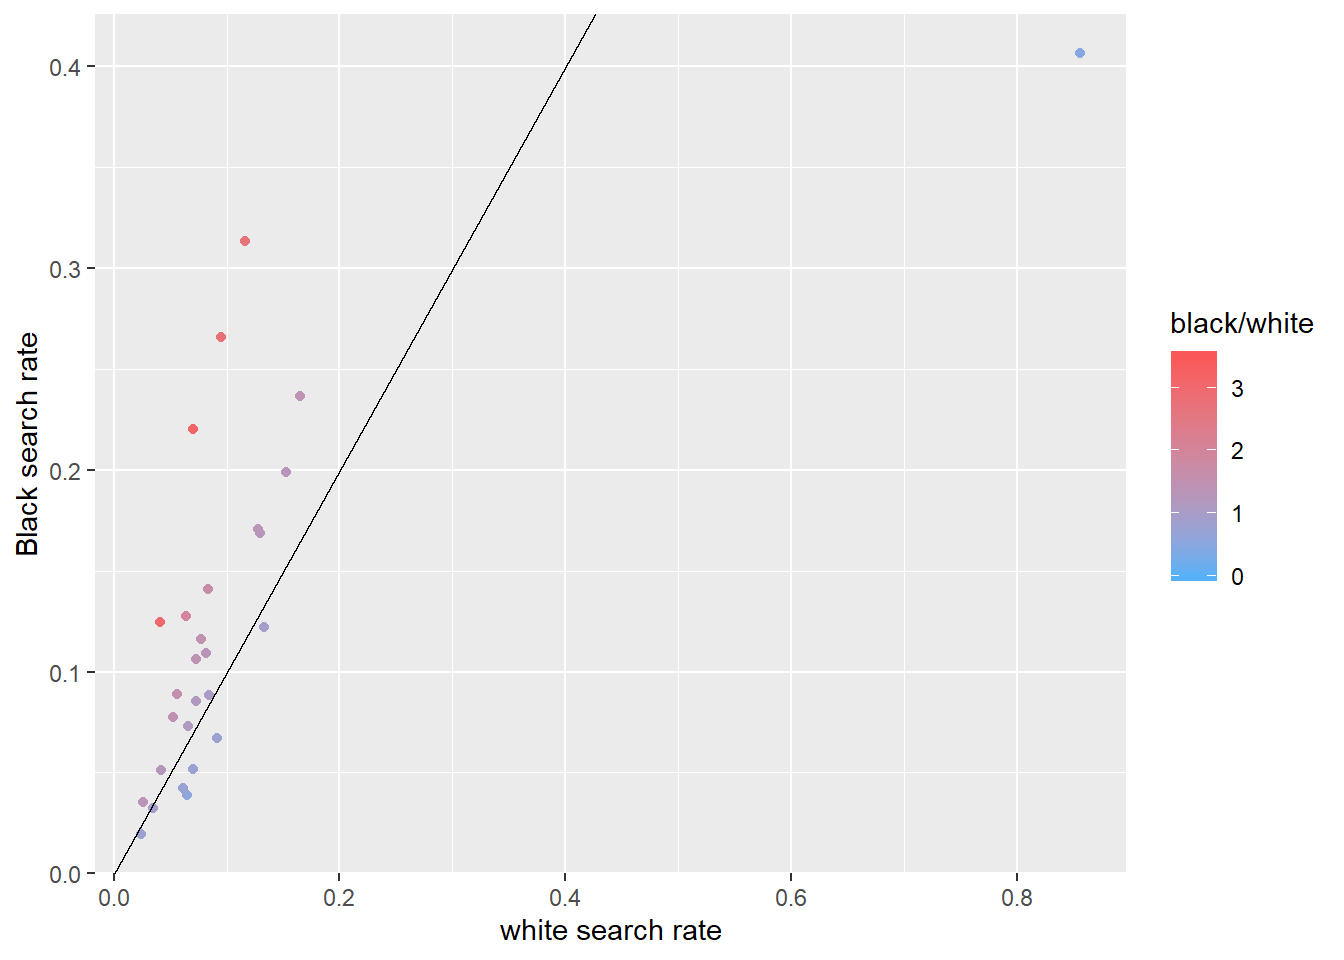
\includegraphics{bookdown-demo_files/figure-latex/unnamed-chunk-68-1.pdf}

The bar chart relays effects of a slew of variables, such as driving behavior of a time of day, time of year, and racial group; traffic and patrol behavior for a given time and location is also relayed. Thus, again, we cannot make definitive statements about racial profiling.

As in the veil of darkness assumption, the race of a motorist is harder to discern during the night than during the day. However, just because the day-night bars in each racial group looks to be about equal neither corroborate nor denies racial profiling. We are without information on the true traffic infringement rate per racial group in different times of the day.

\hypertarget{daynight-outcomes-of-stop-by-race}{%
\subsubsection{Day/night outcomes of stop by race}\label{daynight-outcomes-of-stop-by-race}}

Next, I examine how outcome of stop, race, and day/night interact. I pipe the Oakland data set into ggplot, allowing the color of each bar to represent a traffic stop outcome and the transparency of the bars to denote day and night stops.

\begin{Shaded}
\begin{Highlighting}[]
\CommentTok{# how are outcomes of stops affected by race and time of day?}
  
\NormalTok{CAoak }\OperatorTok
\StringTok{  }\KeywordTok{ggplot}\NormalTok{(}\KeywordTok{aes}\NormalTok{(}\DataTypeTok{x =}\NormalTok{ subject_race, }\DataTypeTok{fill =}\NormalTok{ outcome, }\DataTypeTok{color =}\NormalTok{ outcome, }\DataTypeTok{alpha =}\NormalTok{ light)) }\OperatorTok{+}
\StringTok{  }\KeywordTok{geom_bar}\NormalTok{(}\DataTypeTok{position =} \StringTok{"dodge"}\NormalTok{) }\OperatorTok{+}\StringTok{ }
\StringTok{  }\KeywordTok{scale_alpha_manual}\NormalTok{(}\DataTypeTok{values =} \KeywordTok{c}\NormalTok{(.}\DecValTok{2}\NormalTok{, }\FloatTok{.9}\NormalTok{))}
\end{Highlighting}
\end{Shaded}

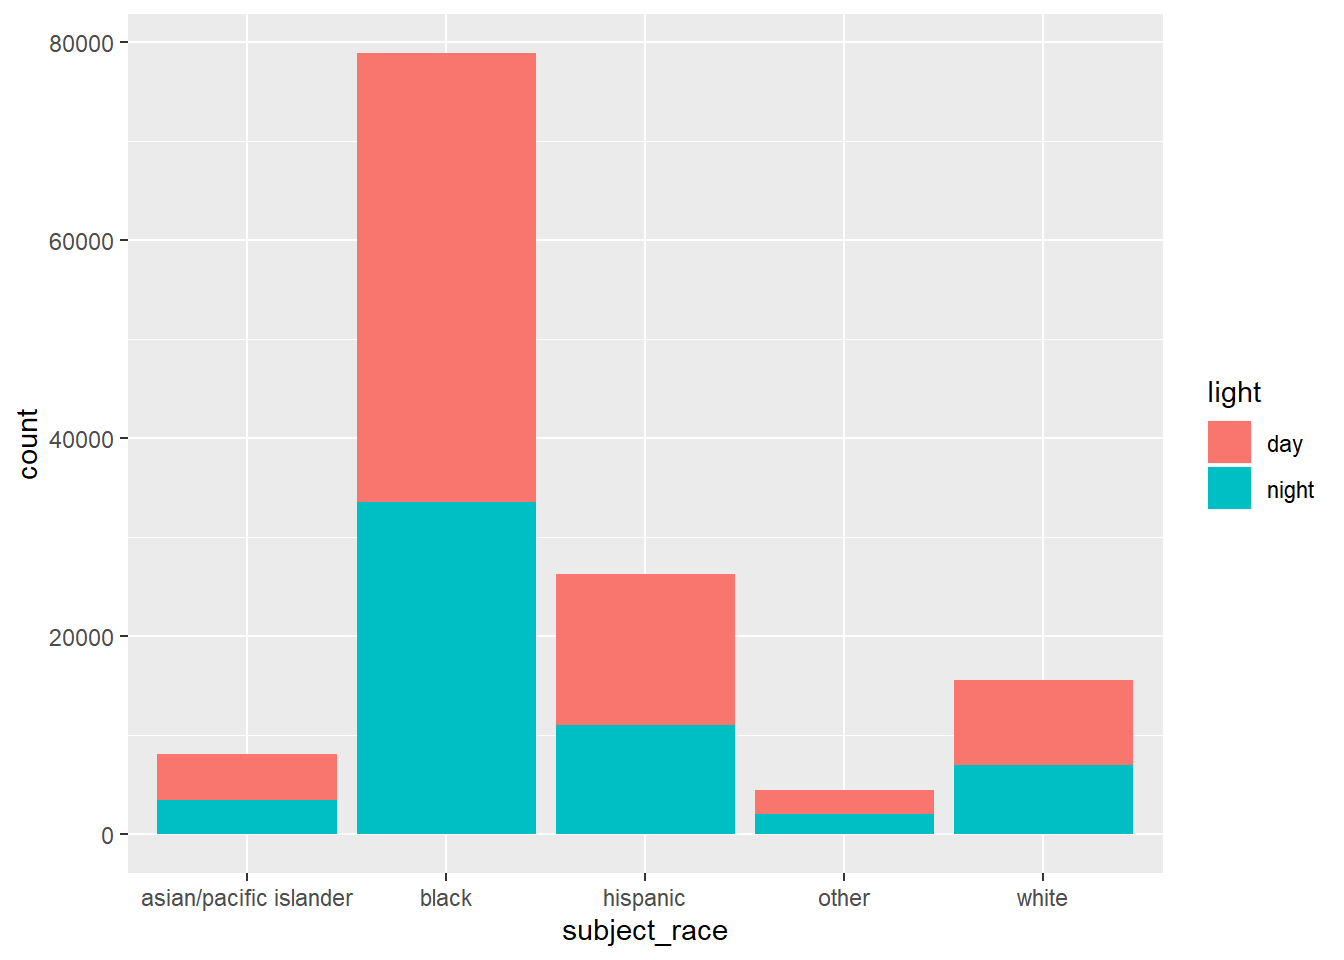
\includegraphics{bookdown-demo_files/figure-latex/unnamed-chunk-69-1.pdf}

Observations:

\begin{itemize}
\item
  For each type of outcome and race, stops during the day outnumber stops during the night. This may result from the Oakland police department's patrol patterns, driver behavior during the day, and/or another factor.
\item
  Missing data regarding traffic outcome does not look to be evenly distributed among stopped motorists -- missing data during the day and night look to be about the same for all racial groups except for Black.
\item
  Citations look to be the most frequent outcome of traffic stops for all racial groups, followed by warning, then arrest (not including missing data.)
\item
  Future directions could look more deeply into the probabilities of each of these outcomes for different racial groups, as the nature of a stricter outcome (being issued a citation rather than a warning) may not be uniformly distributed among racial groups. Furthermore, incorporating the light variable in this direction could be illuminating: are traffic patrols more lenient during the day or during the night once a motorist is stopped? Does the extent of this leniency differ for different racial groups?
\end{itemize}

\hypertarget{dataset-specific-exploration}{%
\section{Dataset-specific Exploration}\label{dataset-specific-exploration}}

\hypertarget{stop-outcomes-in-san-diego}{%
\subsection{Stop outcomes in San Diego}\label{stop-outcomes-in-san-diego}}

\begin{Shaded}
\begin{Highlighting}[]
\NormalTok{CAsd1 <-}\StringTok{ }\NormalTok{DBI}\OperatorTok{::}\KeywordTok{dbGetQuery}\NormalTok{(con1, }\StringTok{"SELECT raw_row_number, arrest_made, citation_issued, warning_issued, search_conducted, search_person, search_vehicle FROM CAsandiego"}\NormalTok{)}
\NormalTok{CAsd2 <-}\StringTok{ }\NormalTok{DBI}\OperatorTok{::}\KeywordTok{dbGetQuery}\NormalTok{(con2, }\StringTok{"SELECT raw_row_number, date, time, service_area, subject_age, subject_race, subject_sex, type, outcome, reason_for_stop, raw_action_taken, raw_subject_race_description FROM CAsandiego"}\NormalTok{)}
\end{Highlighting}
\end{Shaded}

\hypertarget{plotting-count-by-race-over-years-2014-2017}{%
\subsubsection{Plotting Count by Race over years 2014-2017}\label{plotting-count-by-race-over-years-2014-2017}}

\begin{Shaded}
\begin{Highlighting}[]
\NormalTok{goodSD }\OperatorTok\StringTok{ }
\KeywordTok{count}\NormalTok{(}\DataTypeTok{year =} \KeywordTok{year}\NormalTok{(date), raw_subject_race_description) }\OperatorTok\StringTok{ }
\KeywordTok{ggplot}\NormalTok{(}\KeywordTok{aes}\NormalTok{(}\DataTypeTok{x =}\NormalTok{ year, }\DataTypeTok{y =}\NormalTok{ n, }\DataTypeTok{color =}\NormalTok{ raw_subject_race_description)) }\OperatorTok{+}
\KeywordTok{geom_point}\NormalTok{() }\OperatorTok{+}
\KeywordTok{geom_line}\NormalTok{()}
\end{Highlighting}
\end{Shaded}

\begin{verbatim}
## Warning: Removed 1 rows containing missing values (geom_point).
\end{verbatim}

\begin{verbatim}
## Warning: Removed 1 rows containing missing values (geom_path).
\end{verbatim}

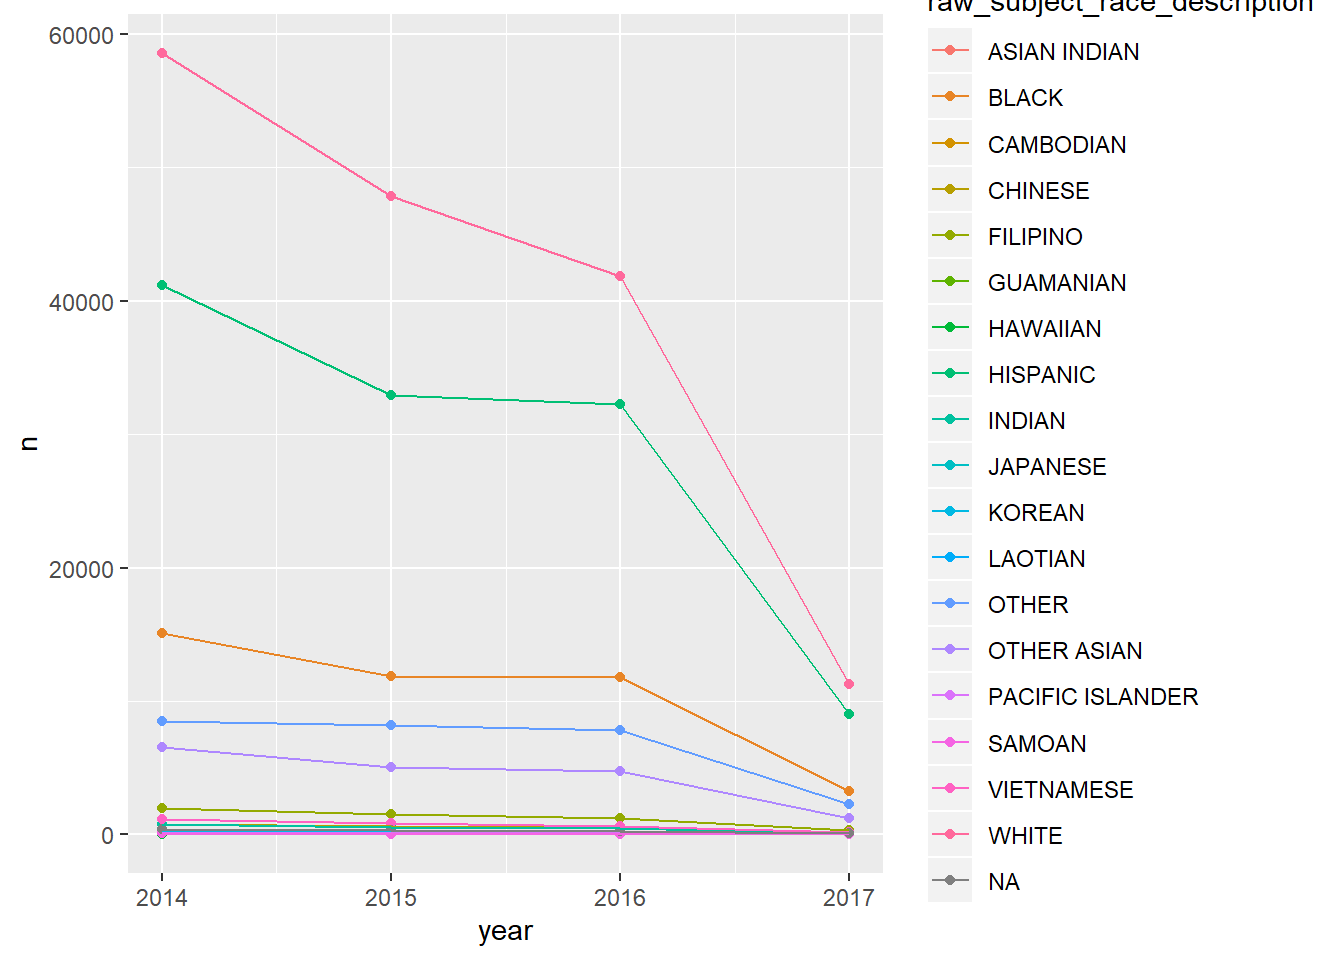
\includegraphics{bookdown-demo_files/figure-latex/unnamed-chunk-74-1.pdf}

\hypertarget{recoding-race-column}{%
\paragraph{Recoding Race column}\label{recoding-race-column}}

\begin{Shaded}
\begin{Highlighting}[]
\CommentTok{# in SD, subject race was very detailed and consistant unlike other datasets}
\CommentTok{# thus, recoded raw_subject_race_description for 'ASIAN/PACIFIC ISLANDER'}
\NormalTok{goodSD}\OperatorTok{$}\NormalTok{raw_subject_race_description <-}\KeywordTok{recode}\NormalTok{(goodSD}\OperatorTok{$}\NormalTok{raw_subject_race_description, }\StringTok{"VIETNAMESE"}\NormalTok{=}\StringTok{"ASIAN/PACIFIC ISLANDER"}\NormalTok{, }
                                \StringTok{"SAMOAN"}\NormalTok{=}\StringTok{"ASIAN/PACIFIC ISLANDER"}\NormalTok{, }
                                \StringTok{"LAOTIAN"}\NormalTok{=}\StringTok{"ASIAN/PACIFIC ISLANDER"}\NormalTok{,}
                                \StringTok{"KOREAN"}\NormalTok{=}\StringTok{"ASIAN/PACIFIC ISLANDER"}\NormalTok{,}
                                \StringTok{"JAPANESE"}\NormalTok{=}\StringTok{"ASIAN/PACIFIC ISLANDER"}\NormalTok{,}
                                \StringTok{"INDIAN"}\NormalTok{=}\StringTok{"ASIAN/PACIFIC ISLANDER"}\NormalTok{,}
                                \StringTok{"HAWAIIAN"}\NormalTok{=}\StringTok{"ASIAN/PACIFIC ISLANDER"}\NormalTok{, }
                                \StringTok{"GUAMANIAN"}\NormalTok{=}\StringTok{"ASIAN/PACIFIC ISLANDER"}\NormalTok{,}
                               \StringTok{"FILIPINO"}\NormalTok{=}\StringTok{"ASIAN/PACIFIC ISLANDER"}\NormalTok{,}
                                \StringTok{"CHINESE"}\NormalTok{=}\StringTok{"ASIAN/PACIFIC ISLANDER"}\NormalTok{,}
                                \StringTok{"CAMBODIAN"}\NormalTok{=}\StringTok{"ASIAN/PACIFIC ISLANDER"}\NormalTok{,}
                               \StringTok{"ASIAN INDIAN"}\NormalTok{=}\StringTok{"ASIAN/PACIFIC ISLANDER"}\NormalTok{,}
                               \StringTok{"OTHER ASIAN"}\NormalTok{=}\StringTok{"ASIAN/PACIFIC ISLANDER"}\NormalTok{,}
                               \StringTok{"PACIFIC ISLANDER"}\NormalTok{=}\StringTok{"ASIAN/PACIFIC ISLANDER"}\NormalTok{)}
\end{Highlighting}
\end{Shaded}

\hypertarget{plotting-search-conducted-by-race}{%
\subsubsection{Plotting Search Conducted by Race}\label{plotting-search-conducted-by-race}}

It is helpful to look at the distribution of stop outcomes because it could suggest underlying intent from the officer or commonalities in policing different races (i.e.~prevalence of profiled searches, warrant for arrest). The following two visualizations display the distribution of searches and arrests made on traffic stops in San Diego.

\begin{Shaded}
\begin{Highlighting}[]
\CommentTok{# create a new dataset}
\NormalTok{SearchesByRaceCOL <-}\StringTok{ }\NormalTok{goodSD }\OperatorTok\StringTok{ }
\StringTok{  }
\StringTok{  }\CommentTok{# select race and search_conducted columns}
\StringTok{  }\KeywordTok{group_by}\NormalTok{(raw_subject_race_description, search_conducted) }\OperatorTok
\StringTok{  }
\StringTok{  }\CommentTok{# calculate count for search_conducted by race}
\StringTok{  }\KeywordTok{summarize}\NormalTok{(}\DataTypeTok{Total =}\KeywordTok{n}\NormalTok{()) }\OperatorTok\StringTok{ }
\StringTok{  }\KeywordTok{group_by}\NormalTok{(raw_subject_race_description) }\OperatorTok\StringTok{ }
\StringTok{  }\KeywordTok{mutate}\NormalTok{(}\DataTypeTok{pct=}\NormalTok{Total}\OperatorTok{/}\KeywordTok{sum}\NormalTok{(Total))}
  \KeywordTok{data.table}\NormalTok{(SearchesByRaceCOL)}
\end{Highlighting}
\end{Shaded}

\begin{verbatim}
##     raw_subject_race_description search_conducted  Total        pct
##  1:       ASIAN/PACIFIC ISLANDER            FALSE  31147 0.97203757
##  2:       ASIAN/PACIFIC ISLANDER             TRUE    896 0.02796243
##  3:                        BLACK            FALSE  38217 0.90949548
##  4:                        BLACK             TRUE   3803 0.09050452
##  5:                     HISPANIC            FALSE 108932 0.94456536
##  6:                     HISPANIC             TRUE   6393 0.05543464
##  7:                        OTHER            FALSE  26420 0.98350892
##  8:                        OTHER             TRUE    443 0.01649108
##  9:                        WHITE            FALSE 155130 0.97223006
## 10:                        WHITE             TRUE   4431 0.02776994
## 11:                         <NA>            FALSE   6893 0.95537076
## 12:                         <NA>             TRUE    322 0.04462924
\end{verbatim}

\begin{Shaded}
\begin{Highlighting}[]
\CommentTok{# omit NAs for search_conducted}
\NormalTok{SearchesByRaceCOL <-}\StringTok{ }\KeywordTok{na.omit}\NormalTok{(SearchesByRaceCOL) }
\CommentTok{# visualize proportion of searches to non-search stops}
\KeywordTok{ggplot}\NormalTok{(SearchesByRaceCOL, }\KeywordTok{aes}\NormalTok{(}\DataTypeTok{x=}\NormalTok{raw_subject_race_description, }\DataTypeTok{y=}\NormalTok{pct, }\DataTypeTok{fill=}\NormalTok{search_conducted))}\OperatorTok{+}\StringTok{ }\KeywordTok{geom_col}\NormalTok{() }\OperatorTok{+}\StringTok{ }\KeywordTok{coord_flip}\NormalTok{() }\OperatorTok{+}\StringTok{ }\KeywordTok{ggtitle}\NormalTok{(}\StringTok{"Search Conducted by Race"}\NormalTok{)}
\end{Highlighting}
\end{Shaded}

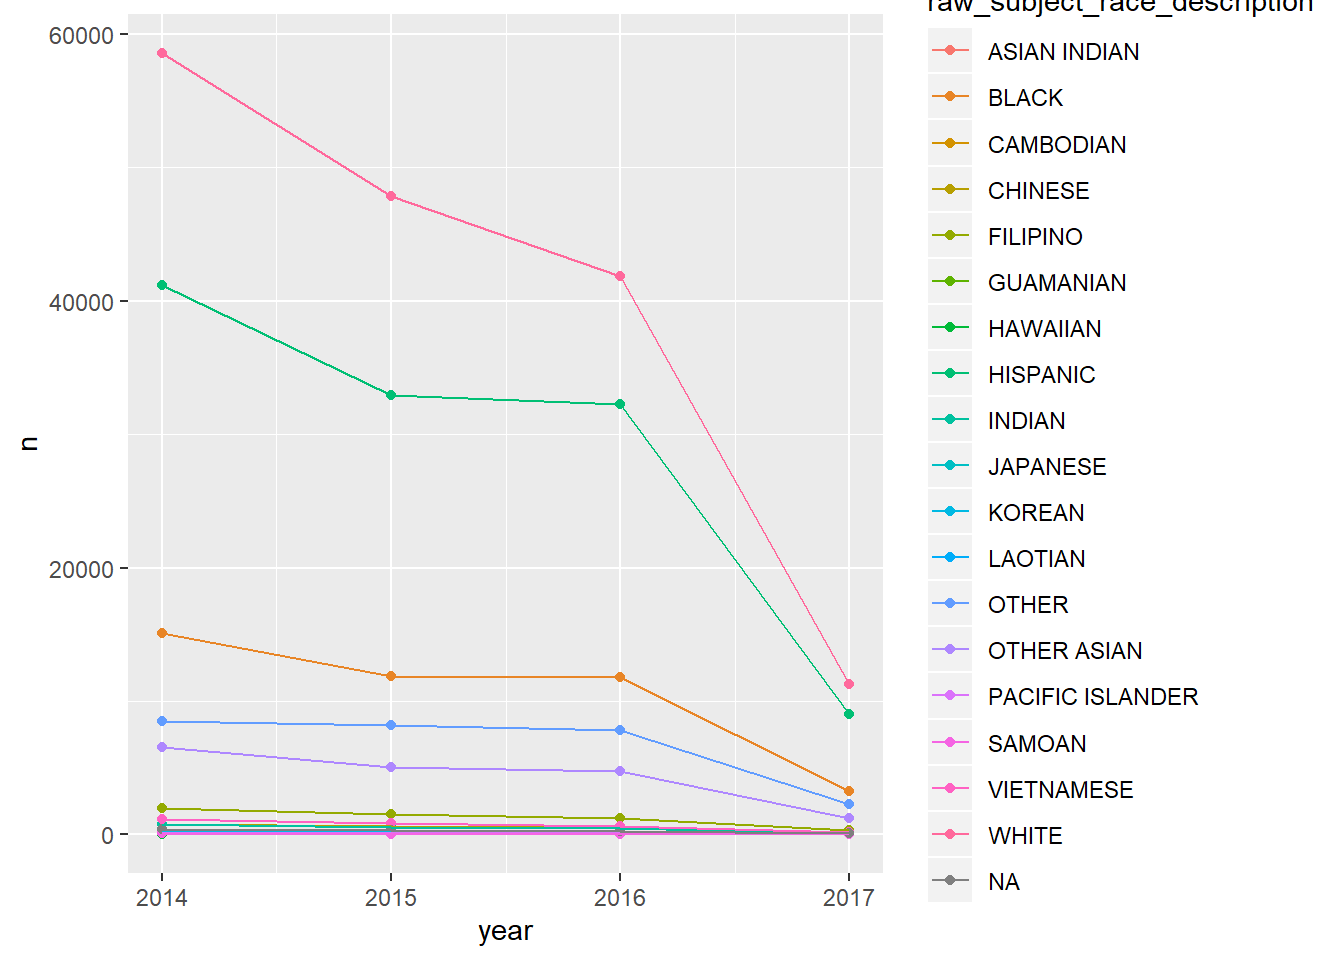
\includegraphics{bookdown-demo_files/figure-latex/unnamed-chunk-76-1.pdf}

\hypertarget{plotting-search-person-by-race}{%
\subsubsection{Plotting Search Person by Race}\label{plotting-search-person-by-race}}

\begin{verbatim}
##     raw_subject_race_description search_person  Total         pct
##  1:       ASIAN/PACIFIC ISLANDER         FALSE  31470 0.982117779
##  2:       ASIAN/PACIFIC ISLANDER            NA    116 0.003620135
##  3:       ASIAN/PACIFIC ISLANDER          TRUE    457 0.014262085
##  4:                        BLACK         FALSE  39630 0.943122323
##  5:                        BLACK            NA    417 0.009923846
##  6:                        BLACK          TRUE   1973 0.046953832
##  7:                     HISPANIC         FALSE 111919 0.970466074
##  8:                     HISPANIC            NA    762 0.006607414
##  9:                     HISPANIC          TRUE   2644 0.022926512
## 10:                        OTHER         FALSE  26630 0.991326360
## 11:                        OTHER            NA     76 0.002829170
## 12:                        OTHER          TRUE    157 0.005844470
## 13:                        WHITE         FALSE 156744 0.982345310
## 14:                        WHITE            NA    755 0.004731733
## 15:                        WHITE          TRUE   2062 0.012922957
## 16:                         <NA>         FALSE   7020 0.972972973
## 17:                         <NA>            NA     64 0.008870409
## 18:                         <NA>          TRUE    131 0.018156618
\end{verbatim}

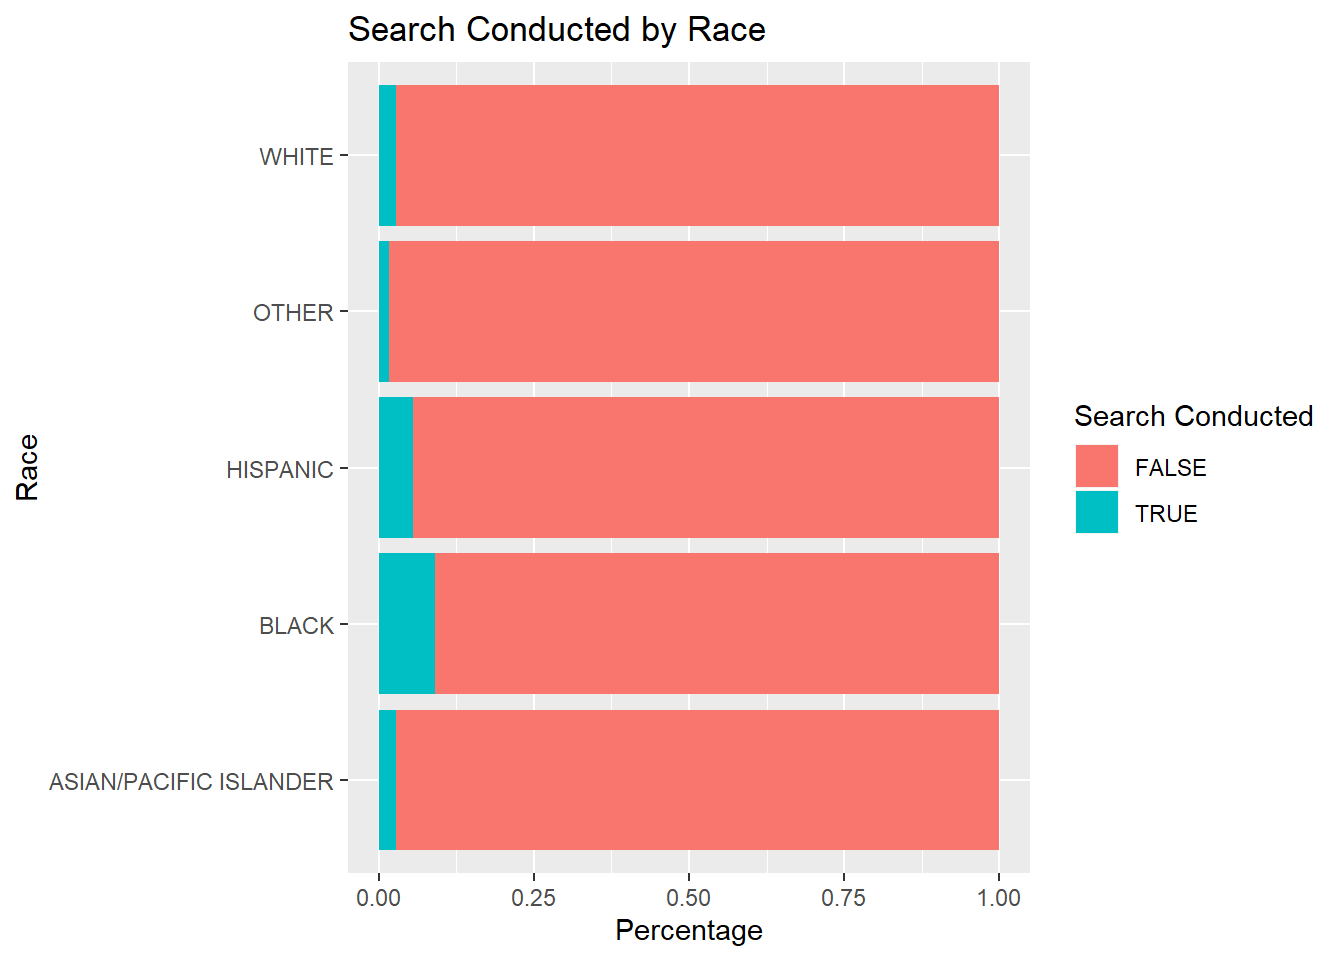
\includegraphics{bookdown-demo_files/figure-latex/unnamed-chunk-77-1.pdf}

\hypertarget{plotting-search-vehicle-by-race}{%
\subsubsection{Plotting Search Vehicle by Race}\label{plotting-search-vehicle-by-race}}

\begin{verbatim}
##     raw_subject_race_description search_vehicle  Total         pct
##  1:       ASIAN/PACIFIC ISLANDER          FALSE  31400 0.979933215
##  2:       ASIAN/PACIFIC ISLANDER             NA    116 0.003620135
##  3:       ASIAN/PACIFIC ISLANDER           TRUE    527 0.016446650
##  4:                        BLACK          FALSE  39200 0.932889100
##  5:                        BLACK             NA    417 0.009923846
##  6:                        BLACK           TRUE   2403 0.057187054
##  7:                     HISPANIC          FALSE 110313 0.956540212
##  8:                     HISPANIC             NA    762 0.006607414
##  9:                     HISPANIC           TRUE   4250 0.036852374
## 10:                        OTHER          FALSE  26513 0.986970927
## 11:                        OTHER             NA     76 0.002829170
## 12:                        OTHER           TRUE    274 0.010199903
## 13:                        WHITE          FALSE 156344 0.979838432
## 14:                        WHITE             NA    755 0.004731733
## 15:                        WHITE           TRUE   2462 0.015429836
## 16:                         <NA>          FALSE   6968 0.965765766
## 17:                         <NA>             NA     64 0.008870409
## 18:                         <NA>           TRUE    183 0.025363825
\end{verbatim}

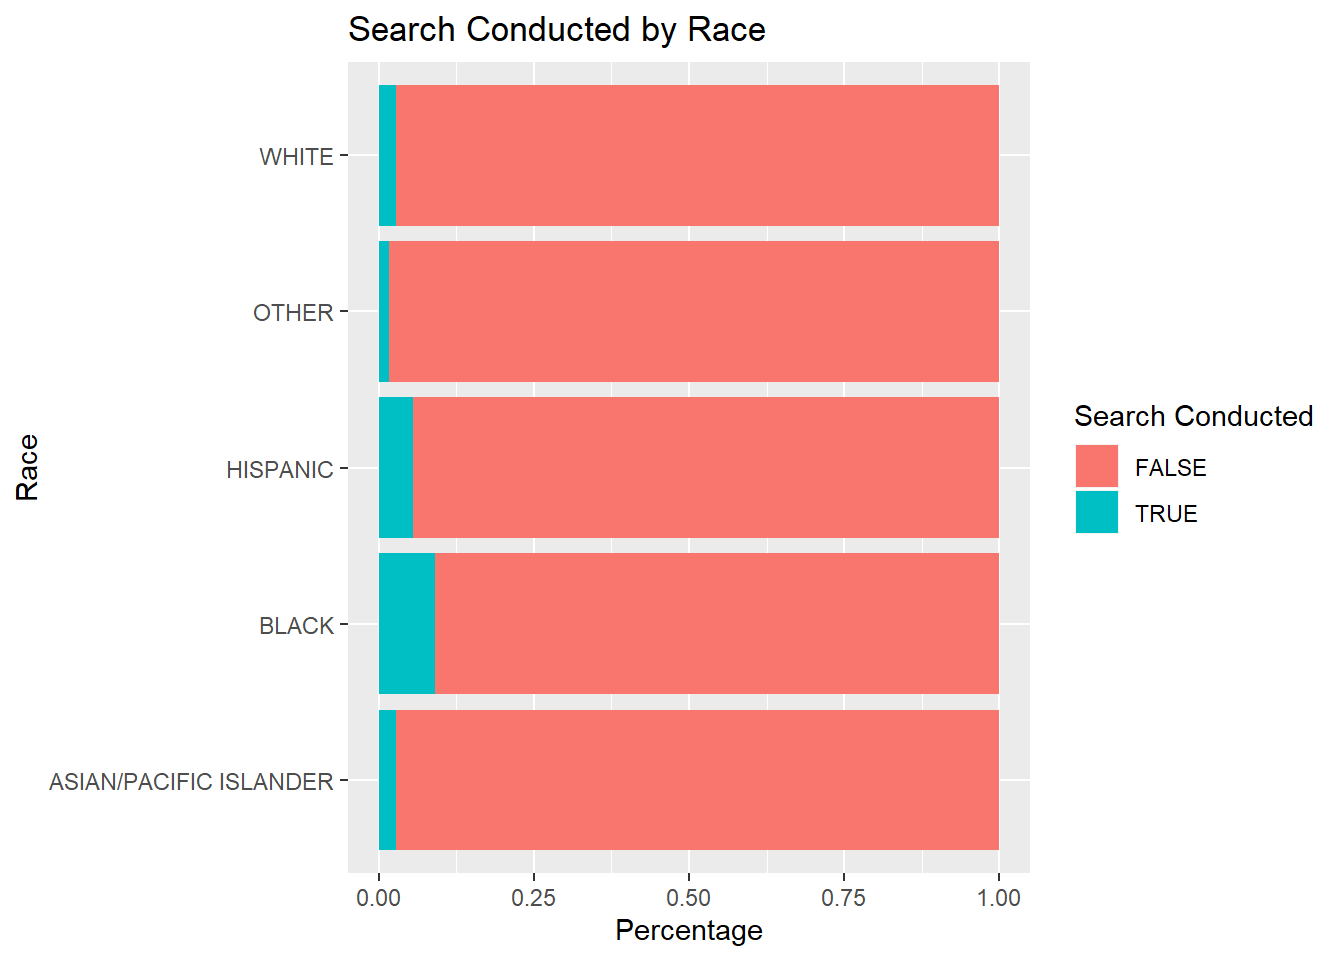
\includegraphics{bookdown-demo_files/figure-latex/unnamed-chunk-78-1.pdf}

\hypertarget{plotting-arrest-made-by-race}{%
\subsubsection{Plotting Arrest Made by Race}\label{plotting-arrest-made-by-race}}

\begin{verbatim}
##     raw_subject_race_description arrest_made  Total         pct
##  1:       ASIAN/PACIFIC ISLANDER       FALSE  29262 0.913210374
##  2:       ASIAN/PACIFIC ISLANDER          NA   2476 0.077271167
##  3:       ASIAN/PACIFIC ISLANDER        TRUE    305 0.009518460
##  4:                        BLACK       FALSE  37953 0.903212756
##  5:                        BLACK          NA   3215 0.076511185
##  6:                        BLACK        TRUE    852 0.020276059
##  7:                     HISPANIC       FALSE 100404 0.870617819
##  8:                     HISPANIC          NA  13224 0.114667245
##  9:                     HISPANIC        TRUE   1697 0.014714936
## 10:                        OTHER       FALSE  24066 0.895879090
## 11:                        OTHER          NA   2638 0.098201988
## 12:                        OTHER        TRUE    159 0.005918922
## 13:                        WHITE       FALSE 145399 0.911243976
## 14:                        WHITE          NA  12416 0.077813501
## 15:                        WHITE        TRUE   1746 0.010942524
## 16:                         <NA>       FALSE   6385 0.884961885
## 17:                         <NA>          NA    774 0.107276507
## 18:                         <NA>        TRUE     56 0.007761608
\end{verbatim}

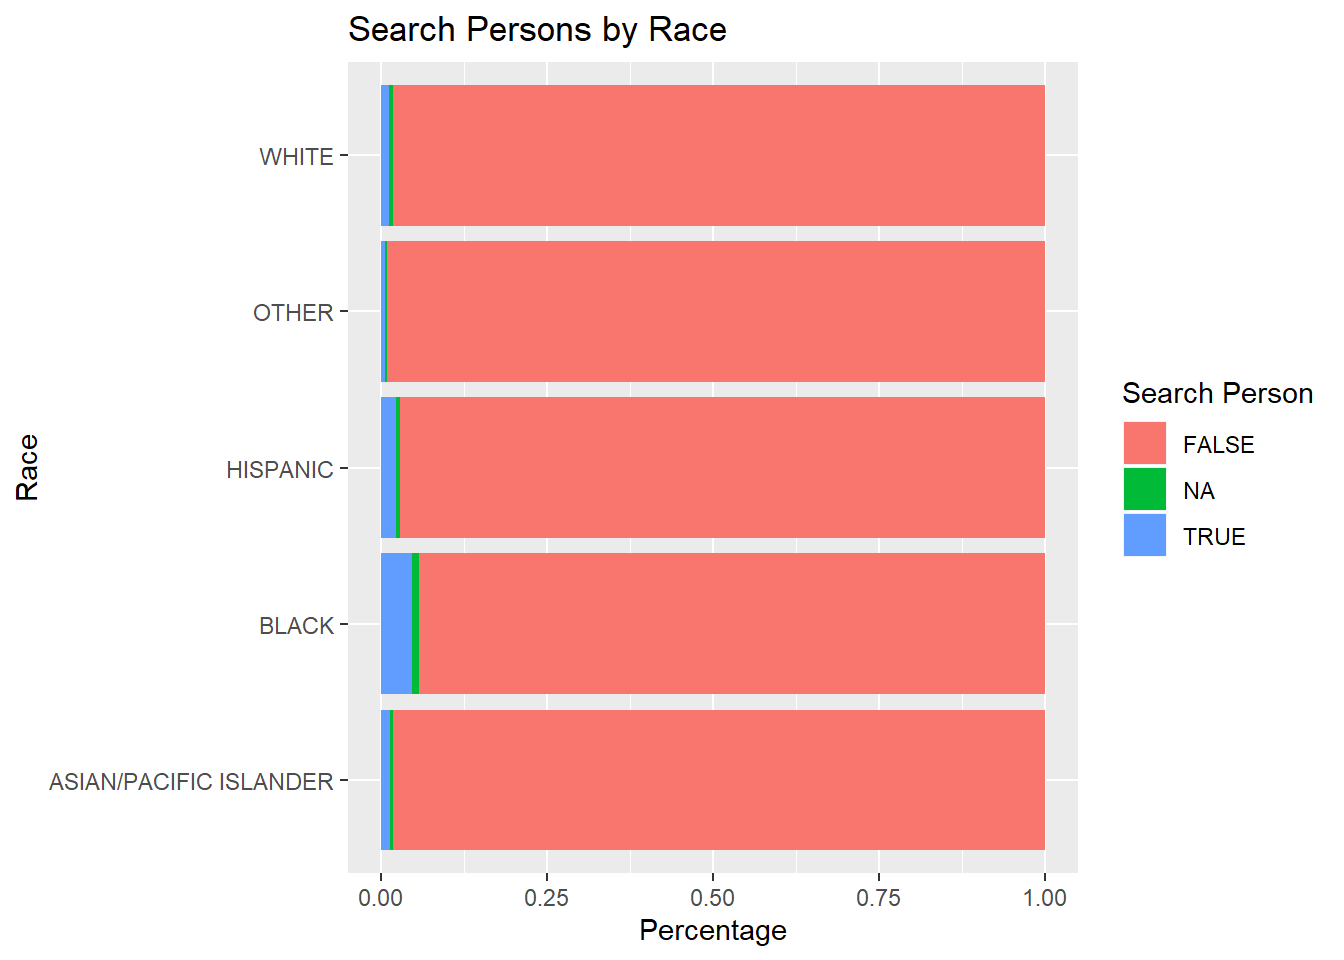
\includegraphics{bookdown-demo_files/figure-latex/unnamed-chunk-79-1.pdf}

\hypertarget{plotting-citations-issued-by-race}{%
\subsubsection{Plotting Citations Issued by Race}\label{plotting-citations-issued-by-race}}

\begin{verbatim}
##     raw_subject_race_description citation_issued Total        pct
##  1:       ASIAN/PACIFIC ISLANDER           FALSE 12496 0.38997597
##  2:       ASIAN/PACIFIC ISLANDER              NA  1937 0.06045002
##  3:       ASIAN/PACIFIC ISLANDER            TRUE 17610 0.54957401
##  4:                        BLACK           FALSE 19105 0.45466445
##  5:                        BLACK              NA  2566 0.06106616
##  6:                        BLACK            TRUE 20349 0.48426940
##  7:                     HISPANIC           FALSE 36667 0.31794494
##  8:                     HISPANIC              NA 12041 0.10440928
##  9:                     HISPANIC            TRUE 66617 0.57764578
## 10:                        OTHER           FALSE  7263 0.27037189
## 11:                        OTHER              NA  2475 0.09213416
## 12:                        OTHER            TRUE 17125 0.63749395
## 13:                        WHITE           FALSE 52240 0.32739830
## 14:                        WHITE              NA 12377 0.07756908
## 15:                        WHITE            TRUE 94944 0.59503262
## 16:                         <NA>           FALSE  2148 0.29771310
## 17:                         <NA>              NA   575 0.07969508
## 18:                         <NA>            TRUE  4492 0.62259182
\end{verbatim}

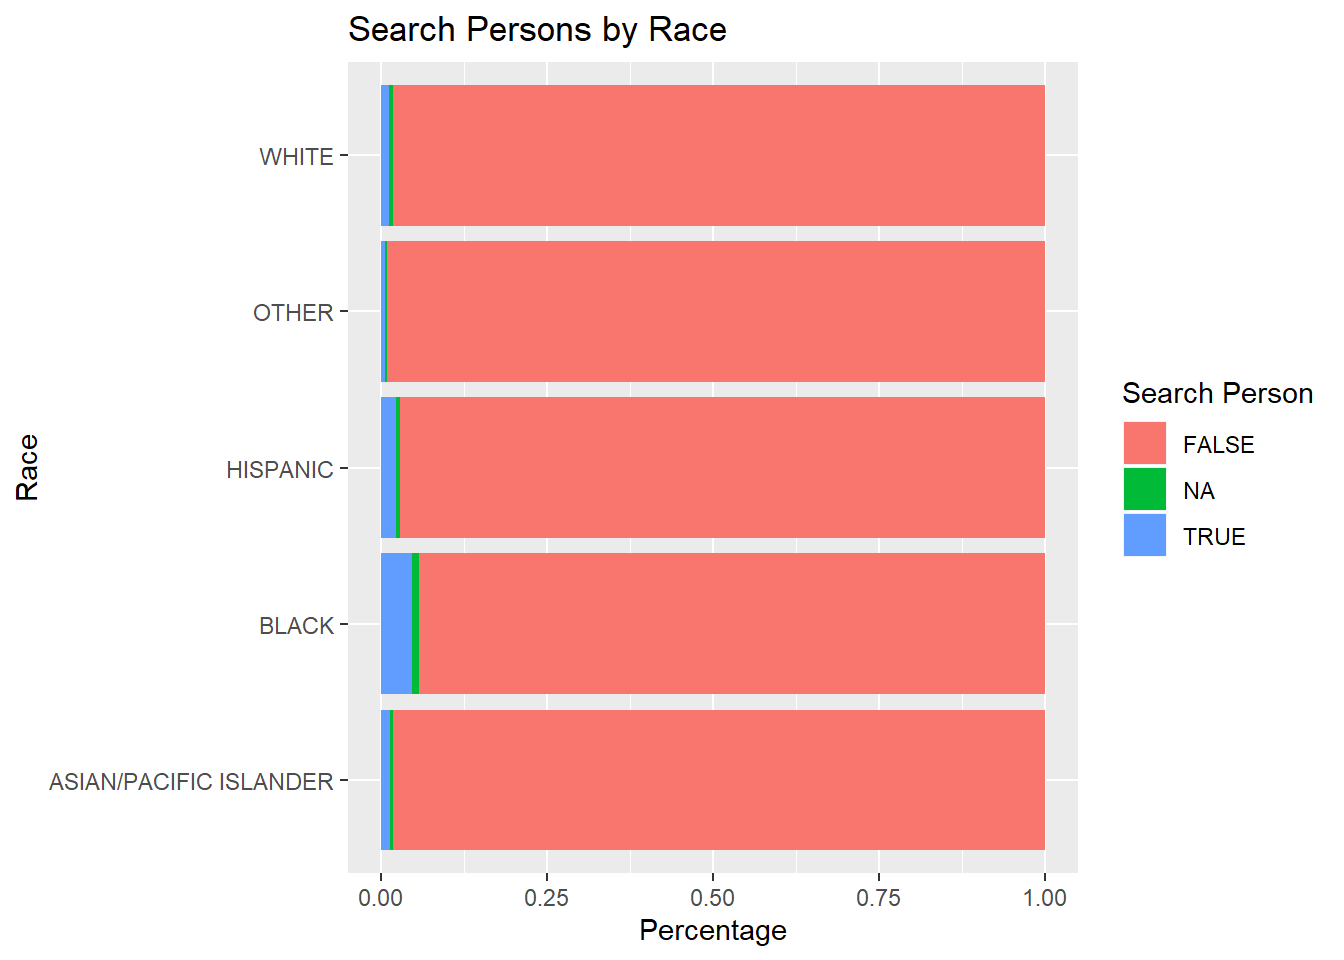
\includegraphics{bookdown-demo_files/figure-latex/unnamed-chunk-80-1.pdf}

\hypertarget{plotting-warnings-issued-by-race}{%
\subsubsection{Plotting Warnings Issued by Race}\label{plotting-warnings-issued-by-race}}

\begin{verbatim}
##     raw_subject_race_description warning_issued Total        pct
##  1:       ASIAN/PACIFIC ISLANDER          FALSE 18313 0.57151328
##  2:       ASIAN/PACIFIC ISLANDER             NA  1937 0.06045002
##  3:       ASIAN/PACIFIC ISLANDER           TRUE 11793 0.36803670
##  4:                        BLACK          FALSE 22953 0.54623989
##  5:                        BLACK             NA  2566 0.06106616
##  6:                        BLACK           TRUE 16501 0.39269396
##  7:                     HISPANIC          FALSE 69890 0.60602645
##  8:                     HISPANIC             NA 12041 0.10440928
##  9:                     HISPANIC           TRUE 33394 0.28956427
## 10:                        OTHER          FALSE 17356 0.64609314
## 11:                        OTHER             NA  2475 0.09213416
## 12:                        OTHER           TRUE  7032 0.26177270
## 13:                        WHITE          FALSE 97389 0.61035591
## 14:                        WHITE             NA 12377 0.07756908
## 15:                        WHITE           TRUE 49795 0.31207501
## 16:                         <NA>          FALSE  4485 0.62162162
## 17:                         <NA>             NA   575 0.07969508
## 18:                         <NA>           TRUE  2155 0.29868330
\end{verbatim}

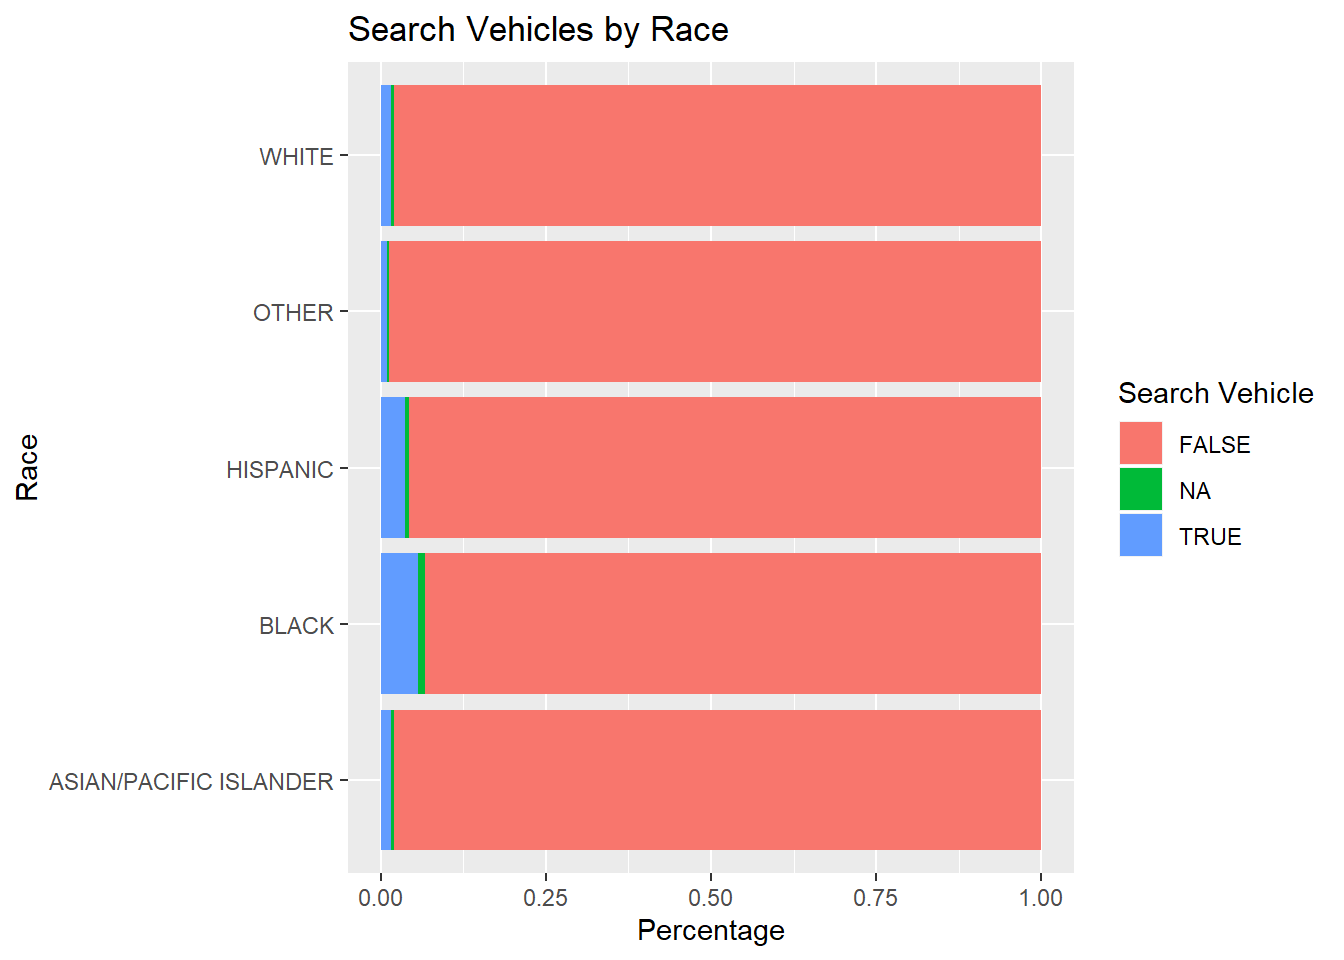
\includegraphics{bookdown-demo_files/figure-latex/unnamed-chunk-81-1.pdf}

\hypertarget{distribution-of-nas-in-outcome-variables}{%
\subsubsection{Distribution of NAs in outcome variables}\label{distribution-of-nas-in-outcome-variables}}

\begin{Shaded}
\begin{Highlighting}[]
\CommentTok{#search_conducted vs. arrest_made, citation_issued, warning_issued}
\KeywordTok{table}\NormalTok{(goodSD}\OperatorTok{$}\NormalTok{search_conducted,goodSD}\OperatorTok{$}\NormalTok{arrest_made)}
\end{Highlighting}
\end{Shaded}

\begin{verbatim}
##        
##          FALSE     NA   TRUE
##   FALSE 331180  34642    917
##   TRUE   12289    101   3898
\end{verbatim}

\begin{Shaded}
\begin{Highlighting}[]
\KeywordTok{table}\NormalTok{(goodSD}\OperatorTok{$}\NormalTok{search_conducted,goodSD}\OperatorTok{$}\NormalTok{citation_issued)}
\end{Highlighting}
\end{Shaded}

\begin{verbatim}
##        
##          FALSE     NA   TRUE
##   FALSE 122819  31235 212685
##   TRUE    7100    736   8452
\end{verbatim}

\begin{Shaded}
\begin{Highlighting}[]
\KeywordTok{table}\NormalTok{(goodSD}\OperatorTok{$}\NormalTok{search_conducted,goodSD}\OperatorTok{$}\NormalTok{warning_issued)}
\end{Highlighting}
\end{Shaded}

\begin{verbatim}
##        
##          FALSE     NA   TRUE
##   FALSE 217781  31235 117723
##   TRUE   12605    736   2947
\end{verbatim}

\begin{Shaded}
\begin{Highlighting}[]
\CommentTok{#search_person vs. arrest_made, citation_issued, warning_issued}
\KeywordTok{table}\NormalTok{(goodSD}\OperatorTok{$}\NormalTok{search_person,goodSD}\OperatorTok{$}\NormalTok{arrest_made)}
\end{Highlighting}
\end{Shaded}

\begin{verbatim}
##        
##          FALSE     NA   TRUE
##   FALSE 337245  34666   1502
##   NA      1483     51    656
##   TRUE    4741     26   2657
\end{verbatim}

\begin{Shaded}
\begin{Highlighting}[]
\KeywordTok{table}\NormalTok{(goodSD}\OperatorTok{$}\NormalTok{search_person,goodSD}\OperatorTok{$}\NormalTok{citation_issued)}
\end{Highlighting}
\end{Shaded}

\begin{verbatim}
##        
##          FALSE     NA   TRUE
##   FALSE 124552  31364 217497
##   NA       756    252   1182
##   TRUE    4611    355   2458
\end{verbatim}

\begin{Shaded}
\begin{Highlighting}[]
\KeywordTok{table}\NormalTok{(goodSD}\OperatorTok{$}\NormalTok{search_person,goodSD}\OperatorTok{$}\NormalTok{warning_issued)}
\end{Highlighting}
\end{Shaded}

\begin{verbatim}
##        
##          FALSE     NA   TRUE
##   FALSE 223434  31364 118615
##   NA      1526    252    412
##   TRUE    5426    355   1643
\end{verbatim}

\begin{Shaded}
\begin{Highlighting}[]
\CommentTok{#search_vehicle vs. arrest_made, citation_issued, warning_issued}
\KeywordTok{table}\NormalTok{(goodSD}\OperatorTok{$}\NormalTok{search_vehicle,goodSD}\OperatorTok{$}\NormalTok{arrest_made)}
\end{Highlighting}
\end{Shaded}

\begin{verbatim}
##        
##          FALSE     NA   TRUE
##   FALSE 333675  34662   2401
##   NA      1483     51    656
##   TRUE    8311     30   1758
\end{verbatim}

\begin{Shaded}
\begin{Highlighting}[]
\KeywordTok{table}\NormalTok{(goodSD}\OperatorTok{$}\NormalTok{search_vehicle,goodSD}\OperatorTok{$}\NormalTok{citation_issued)}
\end{Highlighting}
\end{Shaded}

\begin{verbatim}
##        
##          FALSE     NA   TRUE
##   FALSE 125189  31467 214082
##   NA       756    252   1182
##   TRUE    3974    252   5873
\end{verbatim}

\begin{Shaded}
\begin{Highlighting}[]
\KeywordTok{table}\NormalTok{(goodSD}\OperatorTok{$}\NormalTok{search_vehicle,goodSD}\OperatorTok{$}\NormalTok{warning_issued)}
\end{Highlighting}
\end{Shaded}

\begin{verbatim}
##        
##          FALSE     NA   TRUE
##   FALSE 220741  31467 118530
##   NA      1526    252    412
##   TRUE    8119    252   1728
\end{verbatim}

\begin{Shaded}
\begin{Highlighting}[]
\CommentTok{#What does a conducted search result in?}
\KeywordTok{table}\NormalTok{(goodSD}\OperatorTok{$}\NormalTok{search_conducted,goodSD}\OperatorTok{$}\NormalTok{search_vehicle)}
\end{Highlighting}
\end{Shaded}

\begin{verbatim}
##        
##          FALSE     NA   TRUE
##   FALSE 366739      0      0
##   TRUE    3999   2190  10099
\end{verbatim}

\begin{Shaded}
\begin{Highlighting}[]
\KeywordTok{table}\NormalTok{(goodSD}\OperatorTok{$}\NormalTok{search_conducted,goodSD}\OperatorTok{$}\NormalTok{search_person)}
\end{Highlighting}
\end{Shaded}

\begin{verbatim}
##        
##          FALSE     NA   TRUE
##   FALSE 366739      0      0
##   TRUE    6674   2190   7424
\end{verbatim}

\begin{Shaded}
\begin{Highlighting}[]
\KeywordTok{table}\NormalTok{(goodSD}\OperatorTok{$}\NormalTok{search_person,goodSD}\OperatorTok{$}\NormalTok{search_vehicle)}
\end{Highlighting}
\end{Shaded}

\begin{verbatim}
##        
##          FALSE     NA   TRUE
##   FALSE 366739      0   6674
##   NA         0   2190      0
##   TRUE    3999      0   3425
\end{verbatim}

\begin{Shaded}
\begin{Highlighting}[]
\CommentTok{#NAs in search variables appear to be indicators that search was not designated as a person or vehicle search}
\CommentTok{#three variable plots}
\CommentTok{#looking at traffic stops in relation to income level in the area}
\CommentTok{#dimension reduction: finding what we wanted to predict/model}
\CommentTok{#chugging away at the Shiny app}
\end{Highlighting}
\end{Shaded}

\hypertarget{weather-overlay-in-raleigh}{%
\subsection{Weather Overlay in Raleigh}\label{weather-overlay-in-raleigh}}

This section of exploratory data analysis sees if precipitation shows correlation with the amount of traffic stops per day. The expected correlation is that if it rains more there will be an increase in traffic stops because wet roads could lead to more reckless driving.

The Rnoaa package requires an API key, which can be acquired from the Rnoaa documentation

\hypertarget{visualizing-weather-in-raleigh-north-carolina}{%
\subsubsection{Visualizing Weather in Raleigh, North Carolina}\label{visualizing-weather-in-raleigh-north-carolina}}

In this example, we will overlay precipitation over traffic stops in Raleigh February.

\begin{Shaded}
\begin{Highlighting}[]
\NormalTok{raleigh <-}\StringTok{ }\NormalTok{DBI}\OperatorTok{::}\KeywordTok{dbGetQuery}\NormalTok{(con, }\StringTok{"SELECT * FROM NCraleigh"}\NormalTok{)}
\end{Highlighting}
\end{Shaded}

In order to get weather data we must call the ncdc function. The key argument to keep in mind is the stationid argument. In order to find a city's station ID you must go to this NOAA's website \url{https://www.ncdc.noaa.gov/cdo-web/search}. Moreover, the type of data such as precipation, temperature, and snow etc is contingent on the station ID. For this example, we will look at precipitation only, but there is room to explore more variables to see in any affect traffic.

\begin{Shaded}
\begin{Highlighting}[]
\NormalTok{out <-}\StringTok{ }\KeywordTok{ncdc}\NormalTok{(}\DataTypeTok{datasetid=}\StringTok{'GHCND'}\NormalTok{, }\DataTypeTok{stationid=}\StringTok{'GHCND:USC00317079'}\NormalTok{, }\DataTypeTok{datatypeid=}\StringTok{'PRCP'}\NormalTok{, }\DataTypeTok{startdate =} \StringTok{'2013-01-01'}\NormalTok{, }\DataTypeTok{enddate =} \StringTok{'2013-12-31'}\NormalTok{, }\DataTypeTok{limit =} \DecValTok{500}\NormalTok{)}
\end{Highlighting}
\end{Shaded}

Now that we have the two datasets we must clean them because we will be joining them.

Here we use the lubridate package to make year, month, and day their own columns in the weather dataframe.

\begin{Shaded}
\begin{Highlighting}[]
\NormalTok{weather_df <-}\StringTok{ }\KeywordTok{data.frame}\NormalTok{(out}\OperatorTok{$}\NormalTok{data)}

\CommentTok{# fix weather_df dates}
\NormalTok{weather_df <-}\StringTok{ }\NormalTok{weather_df }\OperatorTok\StringTok{ }\KeywordTok{mutate}\NormalTok{(}\DataTypeTok{clean_date =} \KeywordTok{ymd_hms}\NormalTok{(date))}

\CommentTok{# make individual columns with year, month, & day}
\NormalTok{weather_df <-}\StringTok{ }\NormalTok{weather_df }\OperatorTok
\StringTok{  }\KeywordTok{mutate}\NormalTok{(}\DataTypeTok{year =} \KeywordTok{year}\NormalTok{(clean_date),}
         \DataTypeTok{month =} \KeywordTok{month}\NormalTok{(clean_date),}
         \DataTypeTok{day =} \KeywordTok{day}\NormalTok{(clean_date))}
\end{Highlighting}
\end{Shaded}

Similarly, the raleigh dataset must also have year, month, and day in separate columns.

\begin{Shaded}
\begin{Highlighting}[]
\CommentTok{# use libridate to add clean date column for lubridate to interpret}
\NormalTok{raleigh <-}\StringTok{ }\NormalTok{raleigh }\OperatorTok\StringTok{ }\KeywordTok{mutate}\NormalTok{(}\DataTypeTok{clean_date =} \KeywordTok{ymd}\NormalTok{(date, }\DataTypeTok{tz =} \StringTok{'UTC'}\NormalTok{))}

\CommentTok{# use lubridate to add year, month, day columns}
\NormalTok{raleigh <-}\StringTok{ }\NormalTok{raleigh }\OperatorTok
\StringTok{  }\KeywordTok{mutate}\NormalTok{(}\DataTypeTok{year =} \KeywordTok{year}\NormalTok{(clean_date),}
         \DataTypeTok{month =} \KeywordTok{month}\NormalTok{(clean_date),}
         \DataTypeTok{day =} \KeywordTok{day}\NormalTok{(clean_date))}
\end{Highlighting}
\end{Shaded}

Now that we have the two dataframes cleaned up, we can follow a sequence of piping commands to join and plot them.

\begin{Shaded}
\begin{Highlighting}[]
\CommentTok{# define month variable so we can easily plot different months}
\NormalTok{month_var =}\StringTok{ }\DecValTok{3}
\NormalTok{title =}\StringTok{ }\KeywordTok{paste}\NormalTok{(}\StringTok{"Stop Counts with Arrests and Precipitation Day in 2013-"}\NormalTok{, }\KeywordTok{paste}\NormalTok{(month_var))}
  
\CommentTok{# the pipe sequence below will examine a month in a year such that we count all the traffic}
\CommentTok{# stops that happened that day. Then, we plot the stop counts for a specific day and max temp in}

\NormalTok{raleigh }\OperatorTok\StringTok{ }
\StringTok{  }\CommentTok{# filter out raleigh entries in year 2013 and month variable}
\StringTok{  }\KeywordTok{filter}\NormalTok{(year }\OperatorTok{==}\StringTok{ }\DecValTok{2013}\NormalTok{, month }\OperatorTok{==}\StringTok{ }\NormalTok{month_var, arrest_made}\OperatorTok{==}\StringTok{"TRUE"}\NormalTok{) }\OperatorTok\StringTok{ }
\StringTok{  }\CommentTok{# left_join by 'clean_date' }
\StringTok{  }\KeywordTok{left_join}\NormalTok{(weather_df, }\DataTypeTok{by =} \KeywordTok{c}\NormalTok{(}\StringTok{'clean_date'}\NormalTok{))}\OperatorTok
\StringTok{  }\CommentTok{# Group the data by day as this will be our shared x-axis}
\StringTok{  }\KeywordTok{group_by}\NormalTok{(day.x) }\OperatorTok
\StringTok{  }\CommentTok{# count the number of stops per day and the precipitation value of that day}
\StringTok{  }\KeywordTok{summarize}\NormalTok{(}\DataTypeTok{count =} \KeywordTok{n}\NormalTok{(), }\DataTypeTok{precipitation=}\KeywordTok{max}\NormalTok{(value)) }\OperatorTok
\StringTok{  }\KeywordTok{ggplot}\NormalTok{() }\OperatorTok{+}\StringTok{ }
\StringTok{  }\KeywordTok{geom_line}\NormalTok{(}\KeywordTok{aes}\NormalTok{(}\DataTypeTok{x=}\NormalTok{day.x, }\DataTypeTok{y=}\NormalTok{ precipitation, }\DataTypeTok{color=}\StringTok{"PRCP"}\NormalTok{)) }\OperatorTok{+}
\StringTok{  }\KeywordTok{geom_line}\NormalTok{(}\KeywordTok{aes}\NormalTok{(}\DataTypeTok{x=}\NormalTok{day.x, }\DataTypeTok{y=}\NormalTok{ count}\OperatorTok{/}\NormalTok{.}\DecValTok{05}\NormalTok{, }\DataTypeTok{color =} \StringTok{"Stop Count"}\NormalTok{)) }\OperatorTok{+}\StringTok{  }
\StringTok{  }\KeywordTok{scale_y_continuous}\NormalTok{(}\DataTypeTok{sec.axis =} \KeywordTok{sec_axis}\NormalTok{(}\OperatorTok{~}\NormalTok{.}\OperatorTok{*}\NormalTok{.}\DecValTok{05}\NormalTok{, }\DataTypeTok{name =} \StringTok{"Stop Count"}\NormalTok{)) }\OperatorTok{+}\StringTok{ }
\StringTok{  }\KeywordTok{ggtitle}\NormalTok{(title)}
\end{Highlighting}
\end{Shaded}

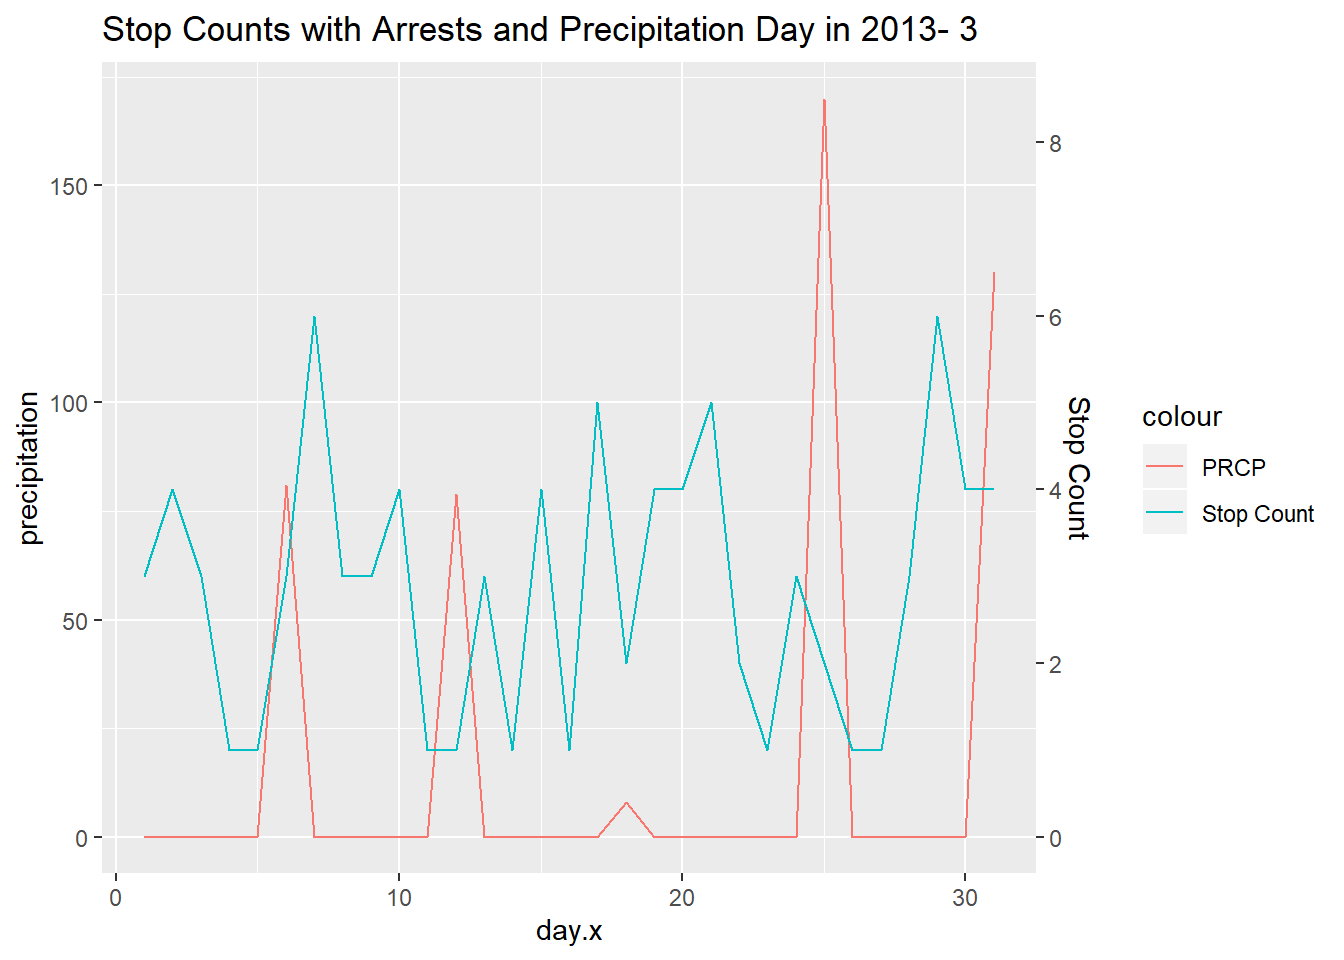
\includegraphics{bookdown-demo_files/figure-latex/unnamed-chunk-91-1.pdf}

Based on the plot, it seems like precipitation in day does not impract the amount of stops. For example, the precipitation day 15 and 25 is relatively but stop count still fluctuates. Future analysis could look at the hourly level of stop counts and precipation or a year long look of precipiation and stop counts per day.

\hypertarget{common-violations-and-map-visualisations-in-san-antonio-tx}{%
\subsection{Common Violations and Map Visualisations in San Antonio, TX}\label{common-violations-and-map-visualisations-in-san-antonio-tx}}

\hypertarget{common-violations}{%
\subsubsection{Common Violations}\label{common-violations}}

Here I graphed the 5 violations that occured most frequently. It is important to notice that this would only include those violations that are worded exactly the same. More work would need to be done in order to find which violations mean the same thing but some had typos or minor differences.

\begin{Shaded}
\begin{Highlighting}[]
\NormalTok{VioData <-}\StringTok{ }\NormalTok{DBI}\OperatorTok{::}\KeywordTok{dbGetQuery}\NormalTok{(con,}
  \StringTok{"SELECT violation, COUNT(violation) AS 'num_violations' FROM TXsanantonio}
\StringTok{  GROUP BY violation}
\StringTok{  ORDER BY `num_violations` DESC}
\StringTok{  LIMIT 5"}\NormalTok{)}

\KeywordTok{ggplot}\NormalTok{(}\DataTypeTok{data =}\NormalTok{ VioData) }\OperatorTok{+}\StringTok{ }\KeywordTok{geom_bar}\NormalTok{(}\DataTypeTok{mapping =} \KeywordTok{aes}\NormalTok{(}\DataTypeTok{x =}\NormalTok{ violation, }\DataTypeTok{y =}\NormalTok{ num_violations), }
                                  \DataTypeTok{stat =} \StringTok{'identity'}\NormalTok{) }\OperatorTok{+}\StringTok{ }\KeywordTok{coord_flip}\NormalTok{()}
\end{Highlighting}
\end{Shaded}

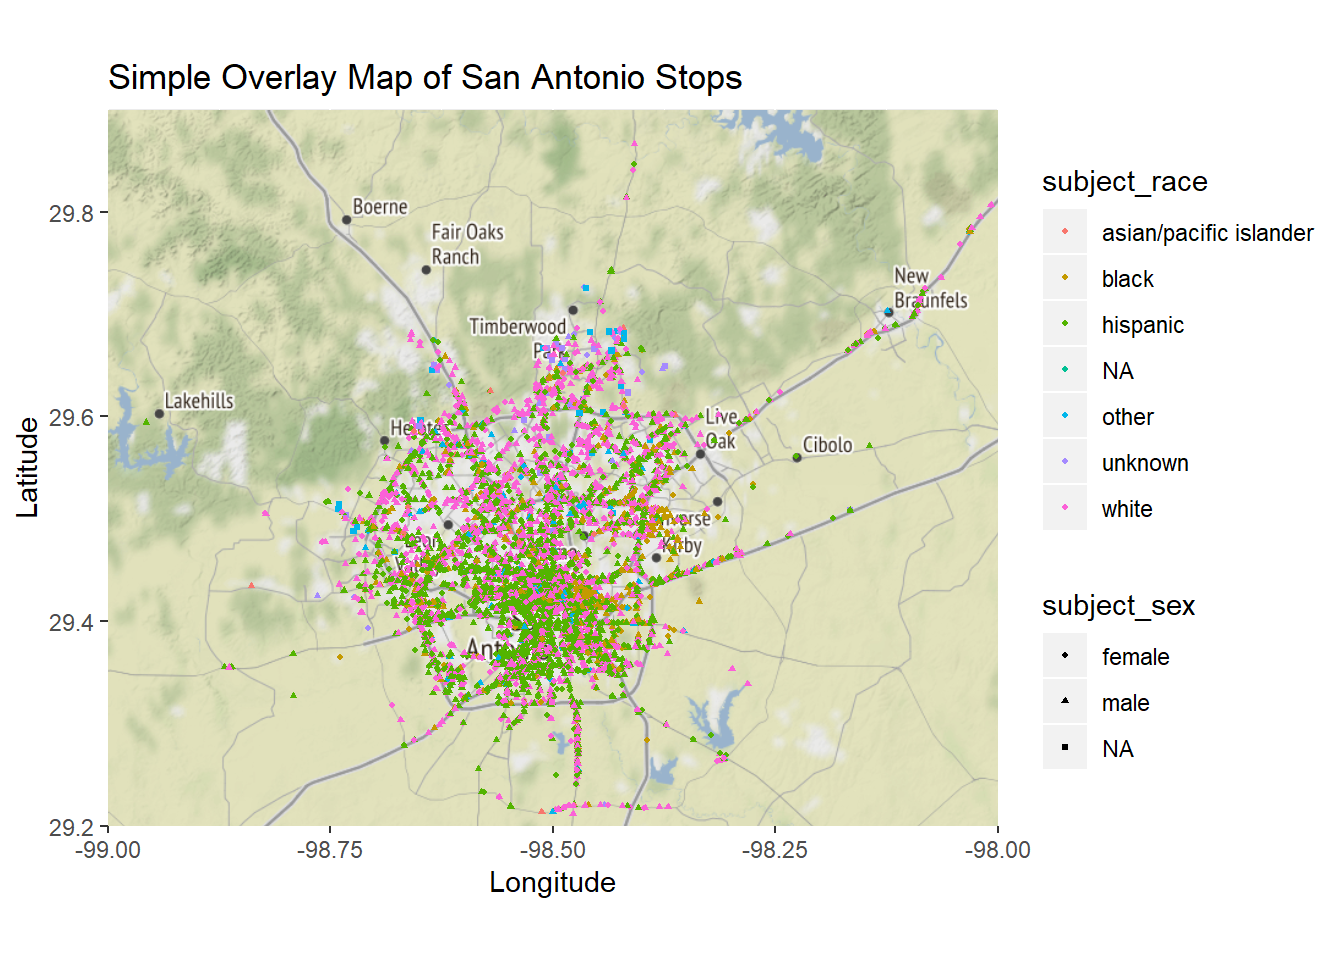
\includegraphics{bookdown-demo_files/figure-latex/unnamed-chunk-100-1.pdf}

I then took these top 5 violations and split them up by sex and race. I also included additional graphs of the 2-5 violations for clarity because of the overwhelming violation of speeding.

\begin{Shaded}
\begin{Highlighting}[]
\NormalTok{top5_vio <-}\StringTok{ }\NormalTok{DBI}\OperatorTok{::}\KeywordTok{dbGetQuery}\NormalTok{(con,}
  \StringTok{"SELECT subject_sex, subject_race, violation FROM TXsanantonio }
\StringTok{  WHERE violation = 'USE OF HAND-HELD MOBILE COMMUNICATION DEVICE' }
\StringTok{  OR violation = 'SPEEDING-POSTED LIMIT' }
\StringTok{  OR violation = 'SPEEDING IN SCHOOL ZONE' }
\StringTok{  OR violation = 'OPERATING A MOTOR VEHICLE WITHOUT A VALID LICENSE' }
\StringTok{  OR violation = 'IMPROPER USE OR FAILURE TO USE SAFETY BELT BY PERS'"}\NormalTok{)}

\NormalTok{top4_vio <-}\StringTok{ }\NormalTok{DBI}\OperatorTok{::}\KeywordTok{dbGetQuery}\NormalTok{(con,}
  \StringTok{"SELECT subject_sex, subject_race, violation FROM TXsanantonio }
\StringTok{  WHERE violation = 'USE OF HAND-HELD MOBILE COMMUNICATION DEVICE' }
\StringTok{  OR violation = 'SPEEDING IN SCHOOL ZONE' }
\StringTok{  OR violation = 'OPERATING A MOTOR VEHICLE WITHOUT A VALID LICENSE' }
\StringTok{  OR violation = 'IMPROPER USE OR FAILURE TO USE SAFETY BELT BY PERS'"}\NormalTok{)}

\KeywordTok{ggplot}\NormalTok{(}\DataTypeTok{data =}\NormalTok{ top5_vio) }\OperatorTok{+}\StringTok{ }\KeywordTok{geom_bar}\NormalTok{(}\DataTypeTok{mapping =} \KeywordTok{aes}\NormalTok{(}\DataTypeTok{x =}\NormalTok{ violation, }\DataTypeTok{fill =}\NormalTok{ subject_race)) }\OperatorTok{+}\StringTok{ }
\StringTok{  }\KeywordTok{coord_flip}\NormalTok{()}
\end{Highlighting}
\end{Shaded}

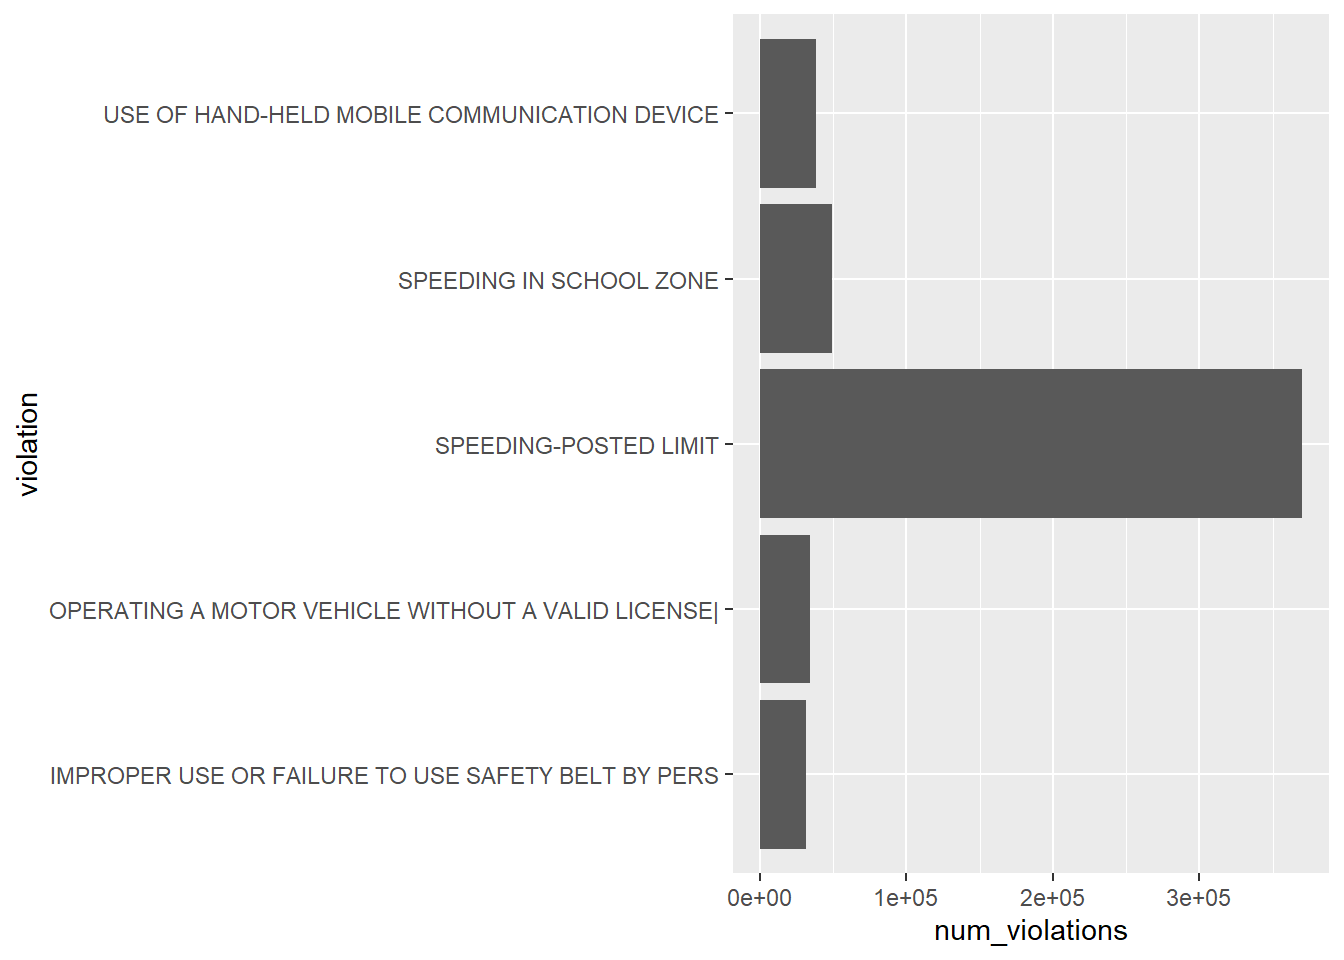
\includegraphics{bookdown-demo_files/figure-latex/unnamed-chunk-101-1.pdf}

\begin{Shaded}
\begin{Highlighting}[]
\CommentTok{#created this to see the 2-5 violations more clearly}
\KeywordTok{ggplot}\NormalTok{(}\DataTypeTok{data =}\NormalTok{ top4_vio) }\OperatorTok{+}\StringTok{ }\KeywordTok{geom_bar}\NormalTok{(}\DataTypeTok{mapping =} \KeywordTok{aes}\NormalTok{(}\DataTypeTok{x =}\NormalTok{ violation, }\DataTypeTok{fill =}\NormalTok{ subject_race)) }\OperatorTok{+}\StringTok{ }
\StringTok{  }\KeywordTok{coord_flip}\NormalTok{()}
\end{Highlighting}
\end{Shaded}

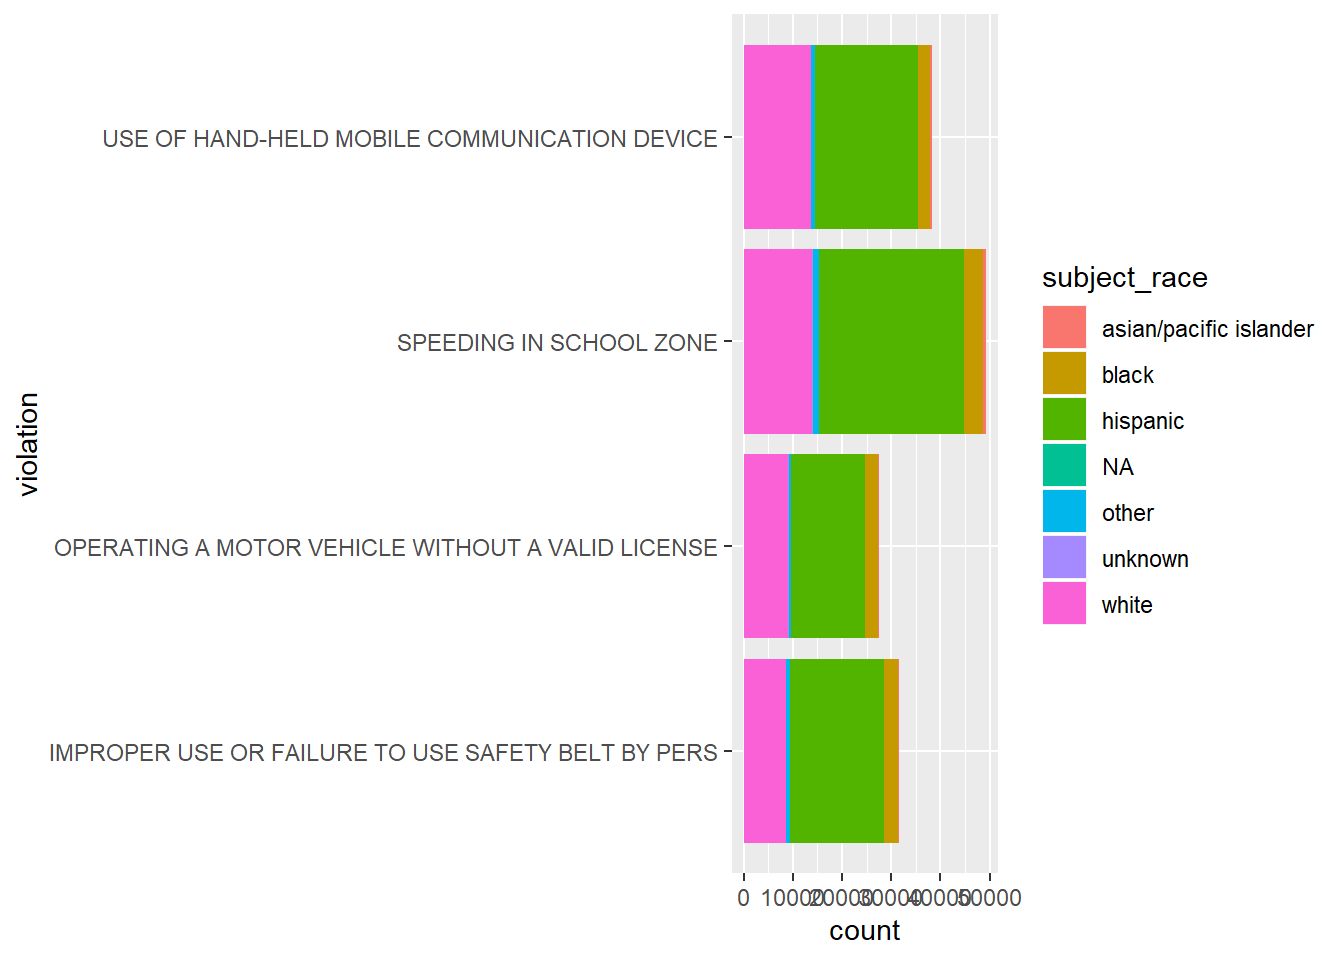
\includegraphics{bookdown-demo_files/figure-latex/unnamed-chunk-101-2.pdf}

\begin{Shaded}
\begin{Highlighting}[]
\KeywordTok{ggplot}\NormalTok{(}\DataTypeTok{data =}\NormalTok{ top5_vio) }\OperatorTok{+}\StringTok{ }\KeywordTok{geom_bar}\NormalTok{(}\DataTypeTok{mapping =} \KeywordTok{aes}\NormalTok{(}\DataTypeTok{x =}\NormalTok{ violation, }\DataTypeTok{fill =}\NormalTok{ subject_sex)) }\OperatorTok{+}\StringTok{ }
\StringTok{  }\KeywordTok{coord_flip}\NormalTok{()}
\end{Highlighting}
\end{Shaded}

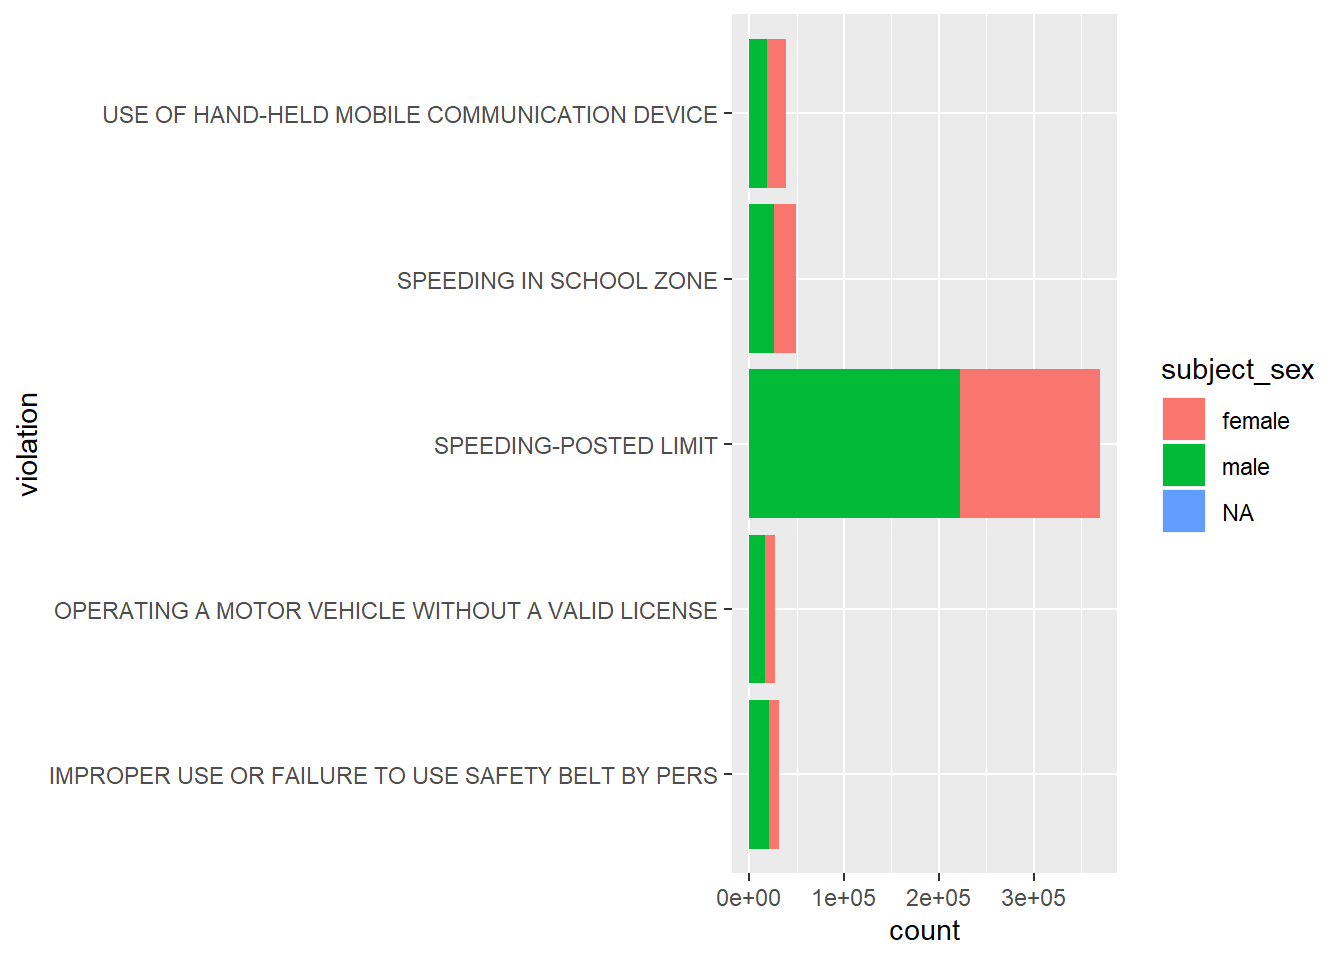
\includegraphics{bookdown-demo_files/figure-latex/unnamed-chunk-101-3.pdf}

\begin{Shaded}
\begin{Highlighting}[]
\CommentTok{#created this to see the 2-5 violations more clearly}
\KeywordTok{ggplot}\NormalTok{(}\DataTypeTok{data =}\NormalTok{ top4_vio) }\OperatorTok{+}\StringTok{ }\KeywordTok{geom_bar}\NormalTok{(}\DataTypeTok{mapping =} \KeywordTok{aes}\NormalTok{(}\DataTypeTok{x =}\NormalTok{ violation, }\DataTypeTok{fill =}\NormalTok{ subject_sex)) }\OperatorTok{+}\StringTok{ }
\StringTok{  }\KeywordTok{coord_flip}\NormalTok{()}
\end{Highlighting}
\end{Shaded}

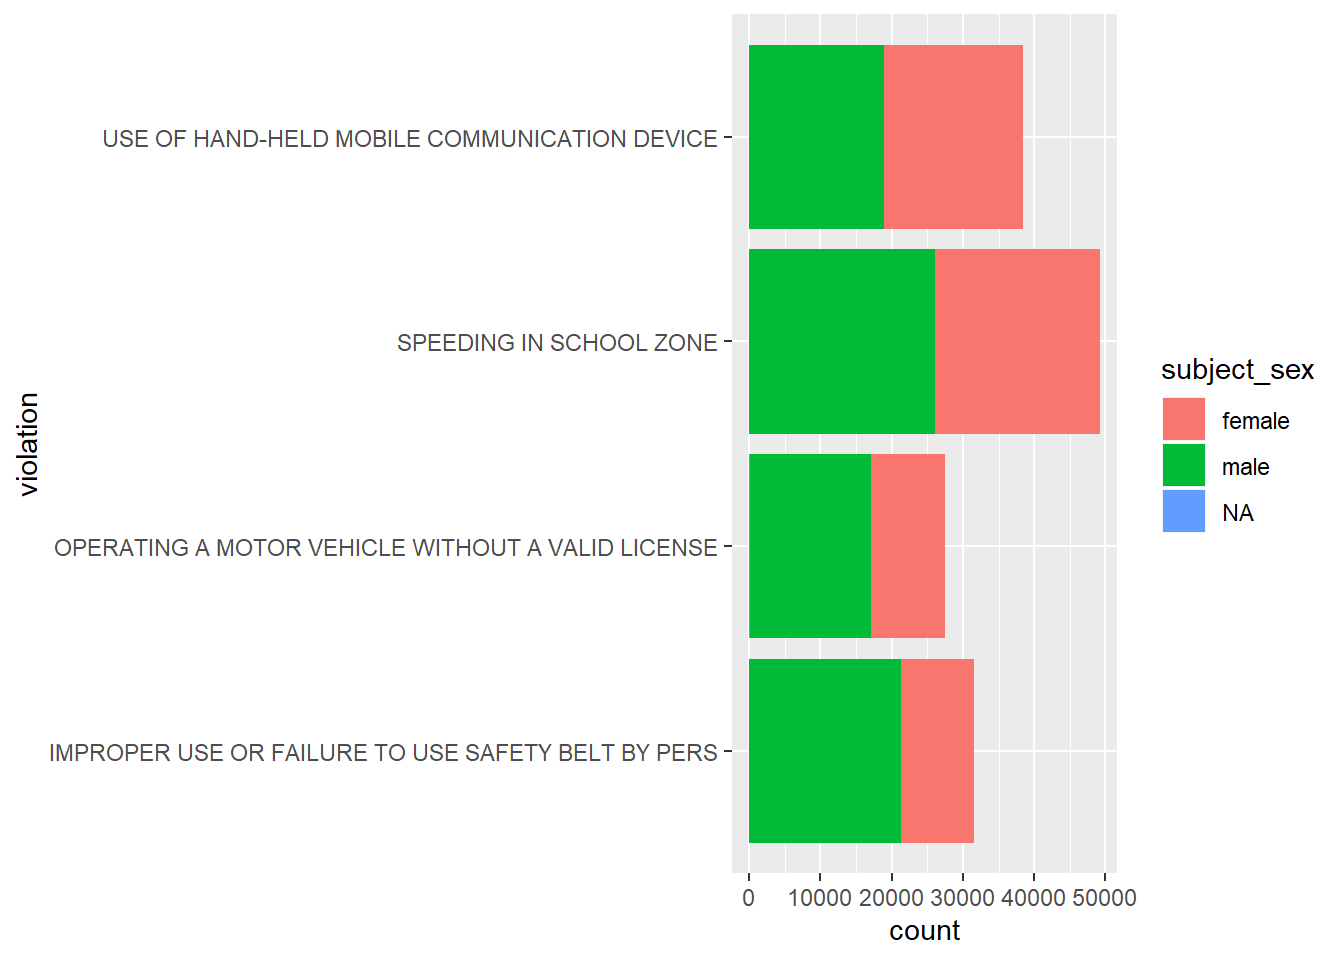
\includegraphics{bookdown-demo_files/figure-latex/unnamed-chunk-101-4.pdf}

\hypertarget{map-overlay}{%
\subsubsection{Map Overlay}\label{map-overlay}}

During the EDA phase, geography became of interest using the latitude and longitude variables from the dataset. This image displays the plot of the San Antonio dataset using ggplot with the dots grouped by the race of the victim of the stop. This raised a few questions. For example, we questioned how highway stops may differ from non highway stops given a potential difference in demographics for those who drive on the highways. We also recognized the possibility of controlling for demographics of certain neighborhoods and comparing stop rates to those demographics. Both questions raise interesting questions for further investigation.

\begin{Shaded}
\begin{Highlighting}[]
\NormalTok{Coordinates <-}\StringTok{ }\NormalTok{DBI}\OperatorTok{::}\KeywordTok{dbGetQuery}\NormalTok{(con,}
  \StringTok{"SELECT * FROM TXsanantonio LIMIT 1000"}\NormalTok{)}

\NormalTok{coor <-}\StringTok{ }\NormalTok{DBI}\OperatorTok{::}\KeywordTok{dbGetQuery}\NormalTok{(con,}
  \StringTok{"SELECT lng, lat, subject_race FROM TXsanantonio LIMIT 1000"}\NormalTok{)}

\NormalTok{coor}\OperatorTok{$}\NormalTok{lng <-}\StringTok{ }\KeywordTok{with}\NormalTok{(coor, }\KeywordTok{as.numeric}\NormalTok{(lng))}
\NormalTok{coor}\OperatorTok{$}\NormalTok{lat <-}\StringTok{ }\KeywordTok{with}\NormalTok{(coor, }\KeywordTok{as.numeric}\NormalTok{(lat))}
  
\NormalTok{race_plot <-}\StringTok{ }\KeywordTok{ggplot}\NormalTok{(Coordinates, }\KeywordTok{aes}\NormalTok{(}\DataTypeTok{x =} \KeywordTok{as.numeric}\NormalTok{(lng), }
                                     \DataTypeTok{y =} \KeywordTok{as.numeric}\NormalTok{(lat), }\DataTypeTok{xaxt =} \StringTok{'n'}\NormalTok{, }\DataTypeTok{yaxt =} \StringTok{'n'}\NormalTok{)) }\OperatorTok{+}\StringTok{ }
\StringTok{  }\KeywordTok{geom_point}\NormalTok{(}\KeywordTok{aes}\NormalTok{(}\DataTypeTok{color =}\NormalTok{ subject_race)) }\OperatorTok{+}\StringTok{ }
\StringTok{  }\KeywordTok{xlab}\NormalTok{(}\StringTok{"Longitude"}\NormalTok{) }\OperatorTok{+}\StringTok{ }\KeywordTok{ylab}\NormalTok{(}\StringTok{"Latitude"}\NormalTok{) }\OperatorTok{+}\StringTok{ }\KeywordTok{coord_quickmap}\NormalTok{()}
\NormalTok{race_plot}
\end{Highlighting}
\end{Shaded}

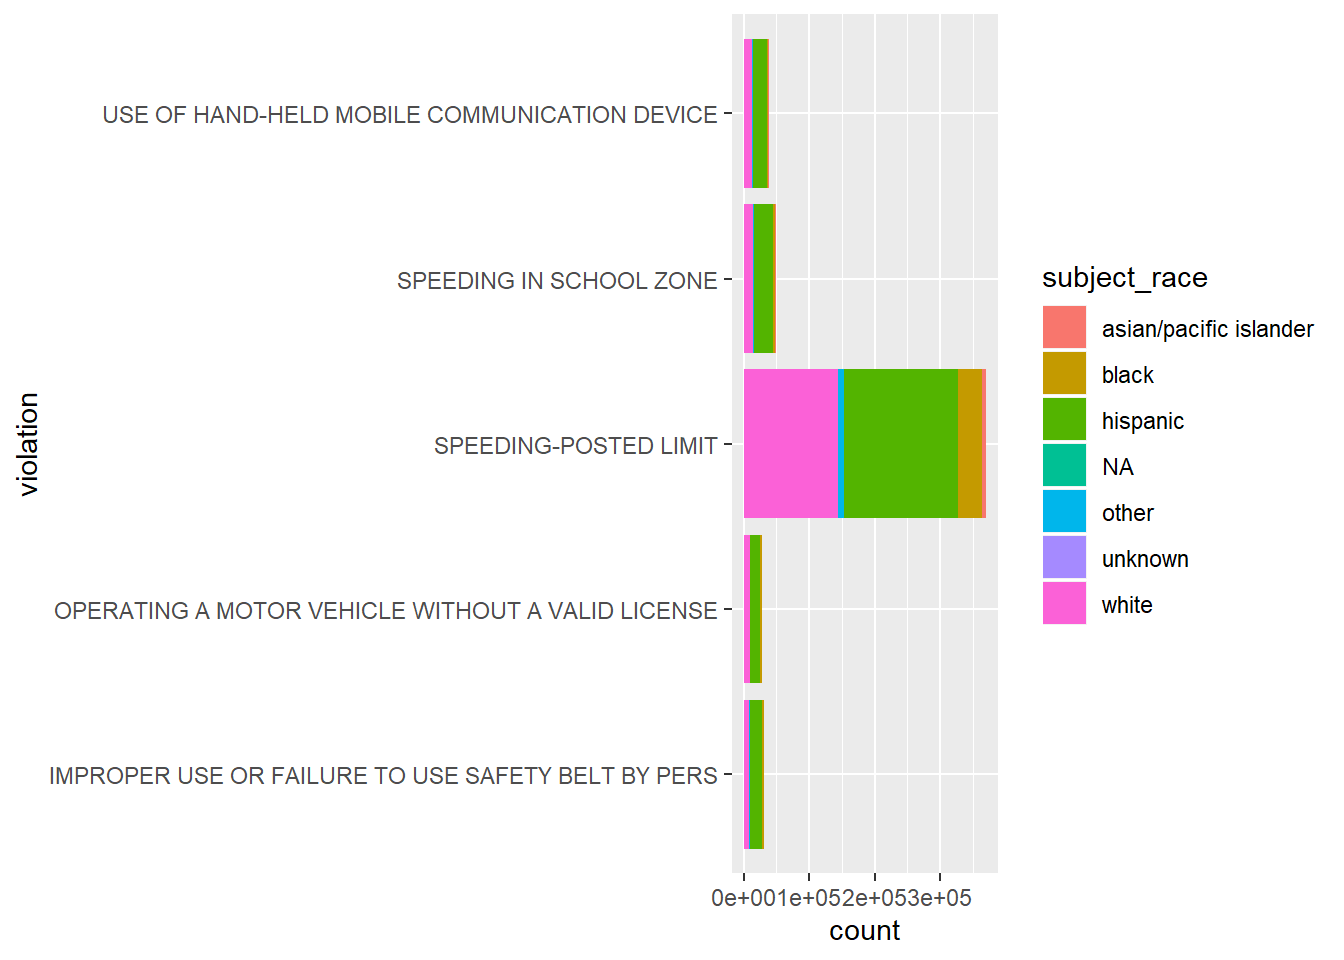
\includegraphics{bookdown-demo_files/figure-latex/unnamed-chunk-102-1.pdf}

\begin{Shaded}
\begin{Highlighting}[]
\NormalTok{coord_plot <-}\StringTok{ }\KeywordTok{qmplot}\NormalTok{(lng, lat, }\DataTypeTok{data =}\NormalTok{ coor, }\DataTypeTok{maptype =} \StringTok{"toner-background"}\NormalTok{, }
                     \DataTypeTok{color =}\NormalTok{ subject_race, }\DataTypeTok{xlim =} \KeywordTok{c}\NormalTok{(}\OperatorTok{-}\DecValTok{99}\NormalTok{, }\FloatTok{-98.25}\NormalTok{), }\DataTypeTok{ylim =} \KeywordTok{c}\NormalTok{(}\DecValTok{29}\NormalTok{, }\FloatTok{29.6}\NormalTok{))}
\NormalTok{coord_plot}
\end{Highlighting}
\end{Shaded}

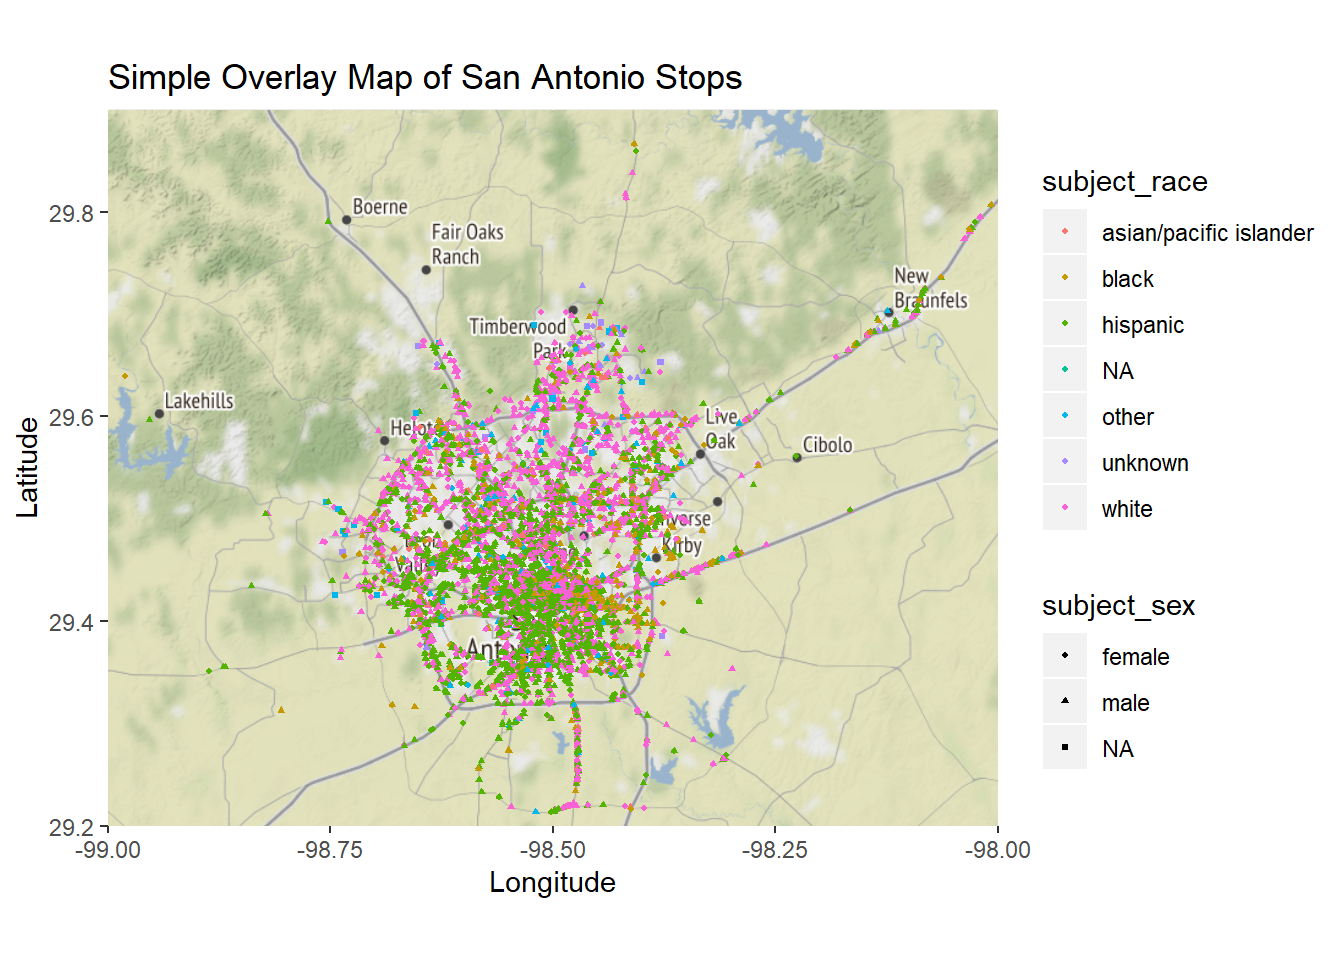
\includegraphics{bookdown-demo_files/figure-latex/unnamed-chunk-103-1.pdf}

\begin{Shaded}
\begin{Highlighting}[]
\KeywordTok{qmplot}\NormalTok{(lng, lat, }\DataTypeTok{data =}\NormalTok{ coor, }\DataTypeTok{maptype =} \StringTok{"toner-background"}\NormalTok{, }
       \DataTypeTok{color =}\NormalTok{ subject_race, }\DataTypeTok{xlim =} \KeywordTok{c}\NormalTok{(}\OperatorTok{-}\FloatTok{98.75}\NormalTok{, }\FloatTok{-98.3}\NormalTok{), }\DataTypeTok{ylim =} \KeywordTok{c}\NormalTok{(}\FloatTok{29.35}\NormalTok{, }\FloatTok{29.5}\NormalTok{))}
\end{Highlighting}
\end{Shaded}

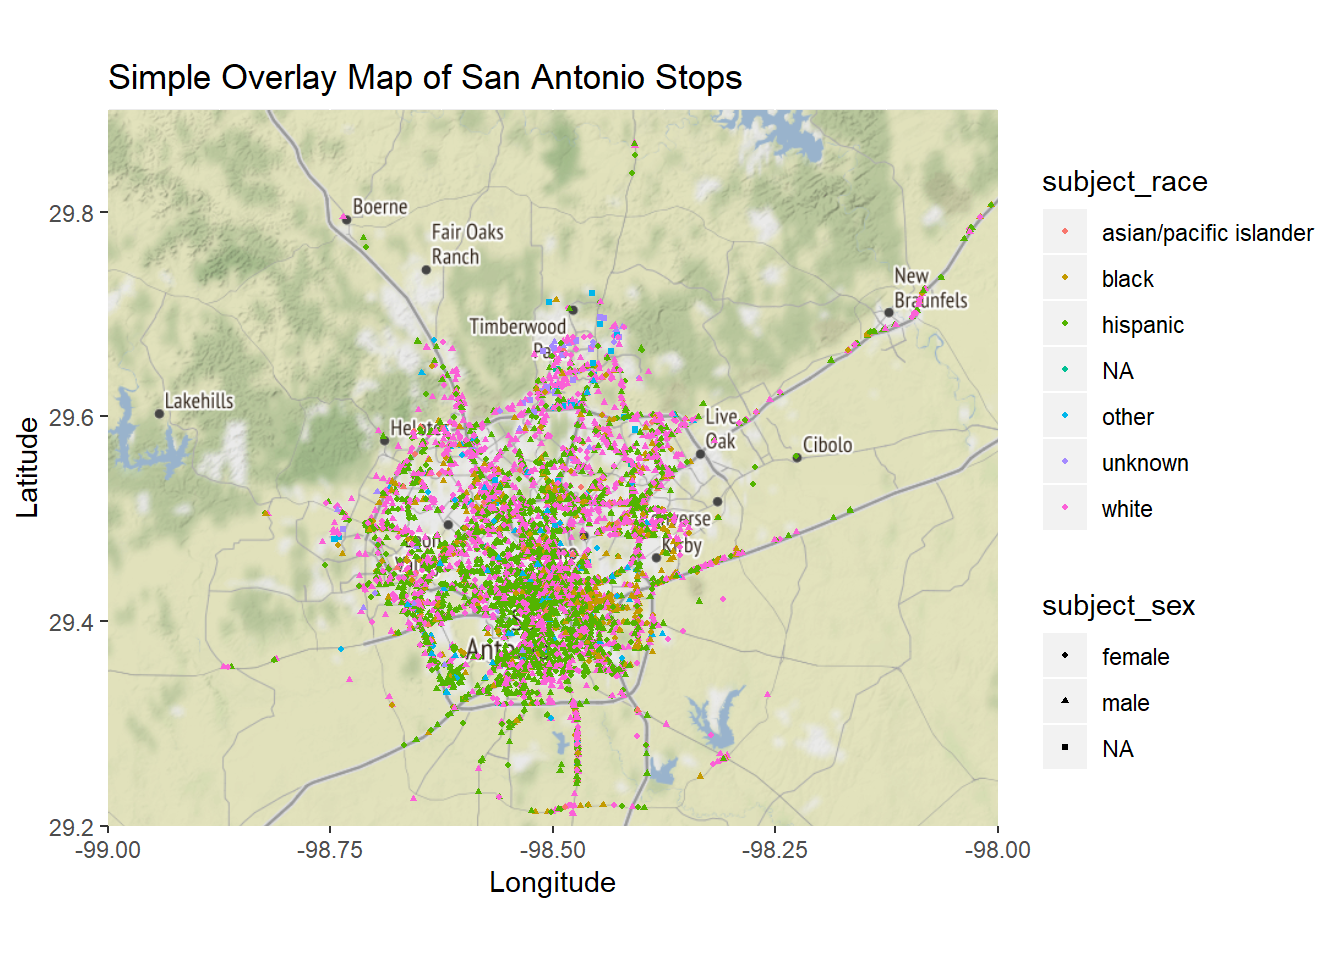
\includegraphics{bookdown-demo_files/figure-latex/unnamed-chunk-104-1.pdf}
This is the same coordinate plot for the Oakland Dataset.

This is a density plot of stops for the oaklans dataset. This was in an attempt to see if there were any particular areas of high concentration.

\begin{Shaded}
\begin{Highlighting}[]
\KeywordTok{qmplot}\NormalTok{(lng, lat, }\DataTypeTok{data =}\NormalTok{ coor2, }\DataTypeTok{geom =} \StringTok{"blank"}\NormalTok{, }
  \DataTypeTok{zoom =} \DecValTok{10}\NormalTok{, }\DataTypeTok{maptype =} \StringTok{"toner-background"}\NormalTok{, }\DataTypeTok{darken =} \DecValTok{0}\NormalTok{, }\DataTypeTok{legend =} \StringTok{"topleft"}\NormalTok{) }\OperatorTok{+}
\StringTok{  }\KeywordTok{stat_density_2d}\NormalTok{(}\KeywordTok{aes}\NormalTok{(}\DataTypeTok{fill =}\NormalTok{ ..level..), }\DataTypeTok{geom =} \StringTok{"polygon"}\NormalTok{, }\DataTypeTok{alpha =} \FloatTok{.5}\NormalTok{, }\DataTypeTok{color =} \OtherTok{NA}\NormalTok{) }\OperatorTok{+}
\StringTok{  }\KeywordTok{scale_fill_gradient2}\NormalTok{(}\StringTok{"Stop}\CharTok{\textbackslash{}n}\StringTok{Propensity"}\NormalTok{, }\DataTypeTok{low =} \StringTok{"white"}\NormalTok{, }\DataTypeTok{mid =} \StringTok{"yellow"}\NormalTok{, }\DataTypeTok{high =} \StringTok{"red"}\NormalTok{, }
                       \DataTypeTok{midpoint =} \DecValTok{100}\NormalTok{)}
\end{Highlighting}
\end{Shaded}

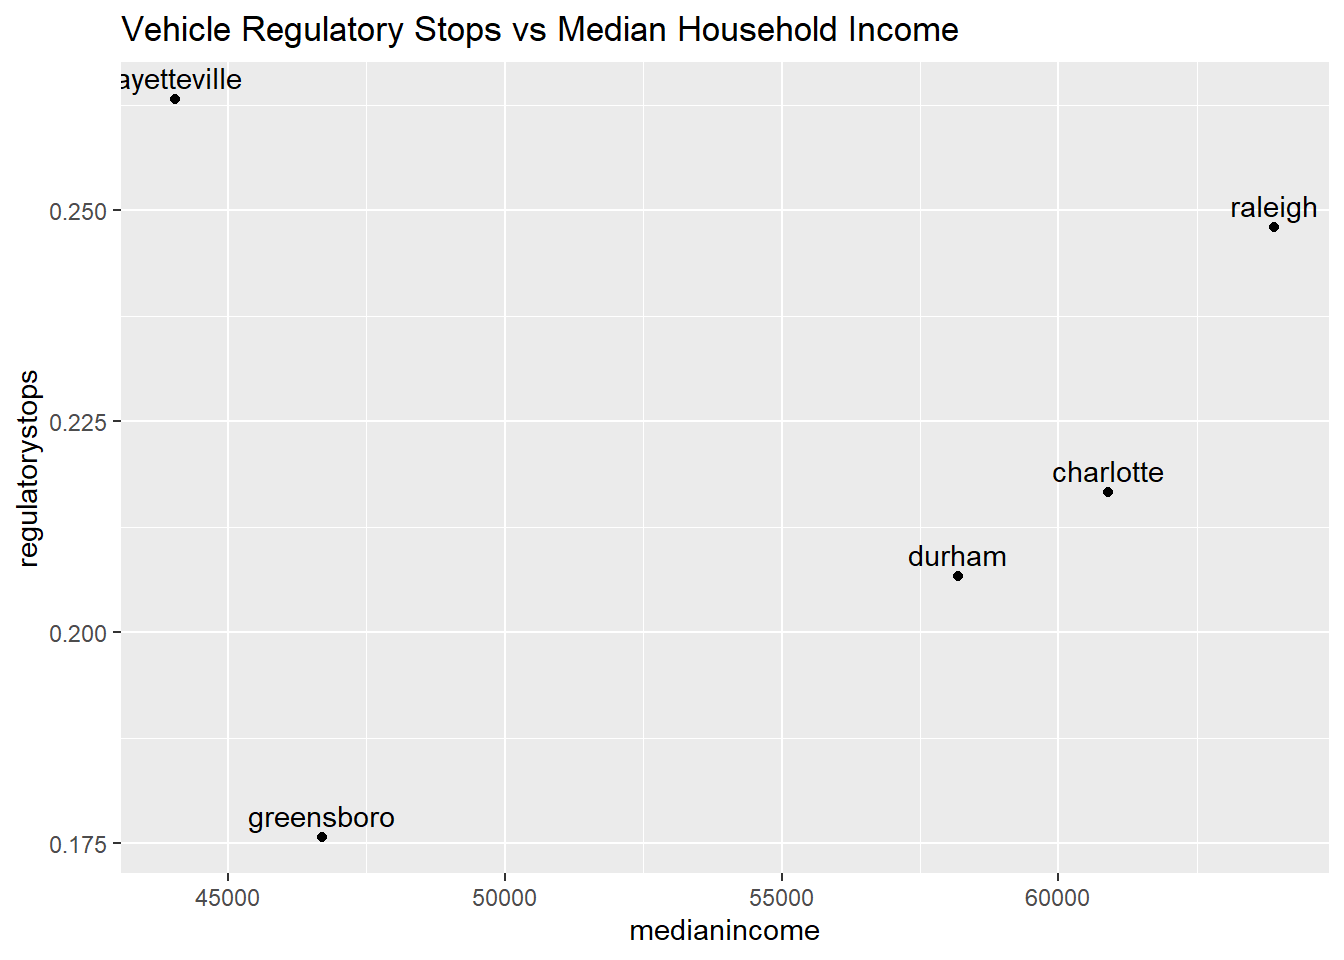
\includegraphics{bookdown-demo_files/figure-latex/unnamed-chunk-106-1.pdf}

\hypertarget{socioeconomic-factors-in-durham}{%
\subsection{Socioeconomic Factors in Durham}\label{socioeconomic-factors-in-durham}}

The reason behind a vehicle equipment stop seems to be an economical one, as drivers who have funds to fix their vehicles in the case of a broken tail light for example would be less likely to get stopped for an equipment violation. The plot is used to investigate this hypothesis, where, as median income increases, we look for the percentage of equipment violations to drop.

\begin{Shaded}
\begin{Highlighting}[]
\CommentTok{#manual data entry}
\NormalTok{incomeNC <-}\StringTok{ }\KeywordTok{data.frame}\NormalTok{(}\StringTok{"city"}\NormalTok{ =}\StringTok{ }\KeywordTok{c}\NormalTok{(}\StringTok{"durham"}\NormalTok{, }\StringTok{"raleigh"}\NormalTok{, }\StringTok{"charlotte"}\NormalTok{, }\StringTok{"fayetteville"}\NormalTok{, }\StringTok{"greensboro"}\NormalTok{), }\StringTok{"medianincome"}\NormalTok{ =}\StringTok{ }\KeywordTok{c}\NormalTok{(}\DecValTok{58190}\NormalTok{, }\DecValTok{63891}\NormalTok{, }\DecValTok{60886}\NormalTok{, }\DecValTok{44057}\NormalTok{, }\DecValTok{46702}\NormalTok{), }\StringTok{"equipmentstops"}\NormalTok{ =}\StringTok{ }\KeywordTok{c}\NormalTok{(}\FloatTok{0.1327}\NormalTok{, }\FloatTok{0.0845}\NormalTok{, }\FloatTok{0.0653}\NormalTok{, }\FloatTok{0.1344}\NormalTok{, }\FloatTok{0.1026}\NormalTok{), }\StringTok{"regulatorystops"}\NormalTok{ =}\StringTok{ }\KeywordTok{c}\NormalTok{(}\FloatTok{0.2067}\NormalTok{, }\FloatTok{0.2480}\NormalTok{, }\FloatTok{0.2166}\NormalTok{, }\FloatTok{0.2632}\NormalTok{, }\FloatTok{0.1758}\NormalTok{))}

\CommentTok{#plot for percent of equipment stops}
\NormalTok{equipment <-}\StringTok{ }\NormalTok{incomeNC }\OperatorTok
\StringTok{  }\KeywordTok{ggplot}\NormalTok{() }\OperatorTok{+}
\StringTok{  }\KeywordTok{geom_point}\NormalTok{(}\KeywordTok{aes}\NormalTok{(}\DataTypeTok{x =}\NormalTok{ medianincome, }\DataTypeTok{y=}\NormalTok{equipmentstops)) }\OperatorTok{+}
\StringTok{  }\KeywordTok{geom_text}\NormalTok{(}\KeywordTok{aes}\NormalTok{(}\DataTypeTok{x =}\NormalTok{ medianincome, }\DataTypeTok{y=}\NormalTok{equipmentstops, }\DataTypeTok{label=}\NormalTok{city),}\DataTypeTok{hjust=}\FloatTok{0.5}\NormalTok{, }\DataTypeTok{vjust=}\OperatorTok{-}\FloatTok{0.5}\NormalTok{) }\OperatorTok{+}
\StringTok{  }\KeywordTok{labs}\NormalTok{(}\DataTypeTok{title=}\StringTok{"Vehicle Equipment Stops vs Median Household Income"}\NormalTok{)}
\NormalTok{equipment }
\end{Highlighting}
\end{Shaded}

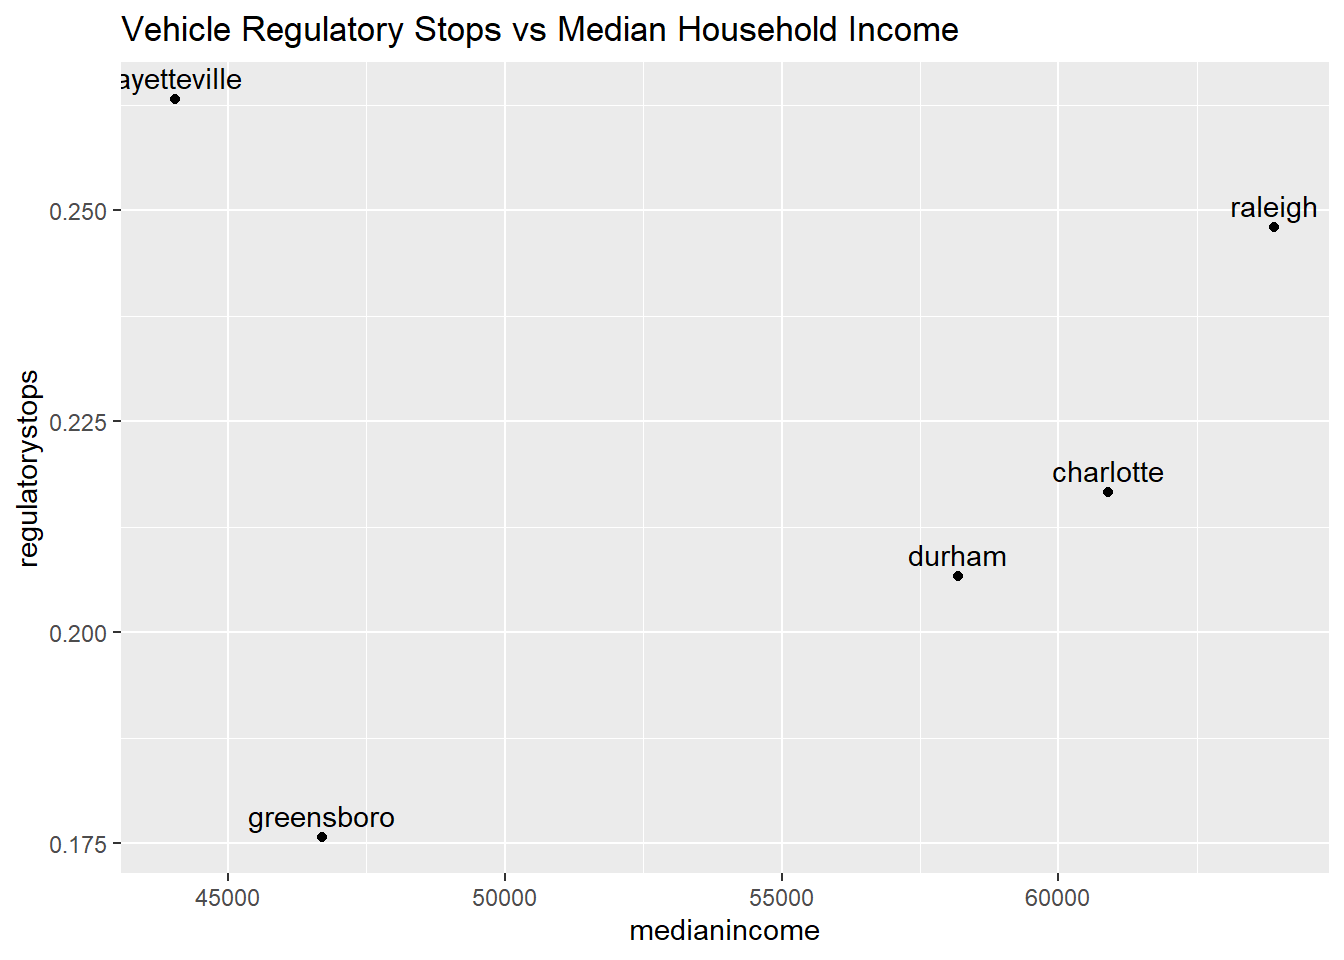
\includegraphics{bookdown-demo_files/figure-latex/unnamed-chunk-110-1.pdf}
This is a scatter plot of percentage of vehicle equipment stops against median household income (obtained from census.gov). The scatter plot reflects this relationship, however since there are so few observations, maybe more data is needed for a more comprehensive conclusion.

\begin{Shaded}
\begin{Highlighting}[]
\CommentTok{#plot for percent of regulatory stops}
\NormalTok{regulatory <-}\StringTok{ }\NormalTok{incomeNC }\OperatorTok
\StringTok{  }\KeywordTok{ggplot}\NormalTok{() }\OperatorTok{+}
\StringTok{  }\KeywordTok{geom_point}\NormalTok{(}\KeywordTok{aes}\NormalTok{(}\DataTypeTok{x =}\NormalTok{ medianincome, }\DataTypeTok{y=}\NormalTok{regulatorystops)) }\OperatorTok{+}
\StringTok{  }\KeywordTok{geom_text}\NormalTok{(}\KeywordTok{aes}\NormalTok{(}\DataTypeTok{x =}\NormalTok{ medianincome, }\DataTypeTok{y=}\NormalTok{regulatorystops, }\DataTypeTok{label=}\NormalTok{city),}\DataTypeTok{hjust=}\FloatTok{0.5}\NormalTok{, }\DataTypeTok{vjust=}\OperatorTok{-}\FloatTok{0.5}\NormalTok{) }\OperatorTok{+}
\StringTok{  }\KeywordTok{labs}\NormalTok{(}\DataTypeTok{title=}\StringTok{"Vehicle Regulatory Stops vs Median Household Income"}\NormalTok{)}
\NormalTok{regulatory}
\end{Highlighting}
\end{Shaded}

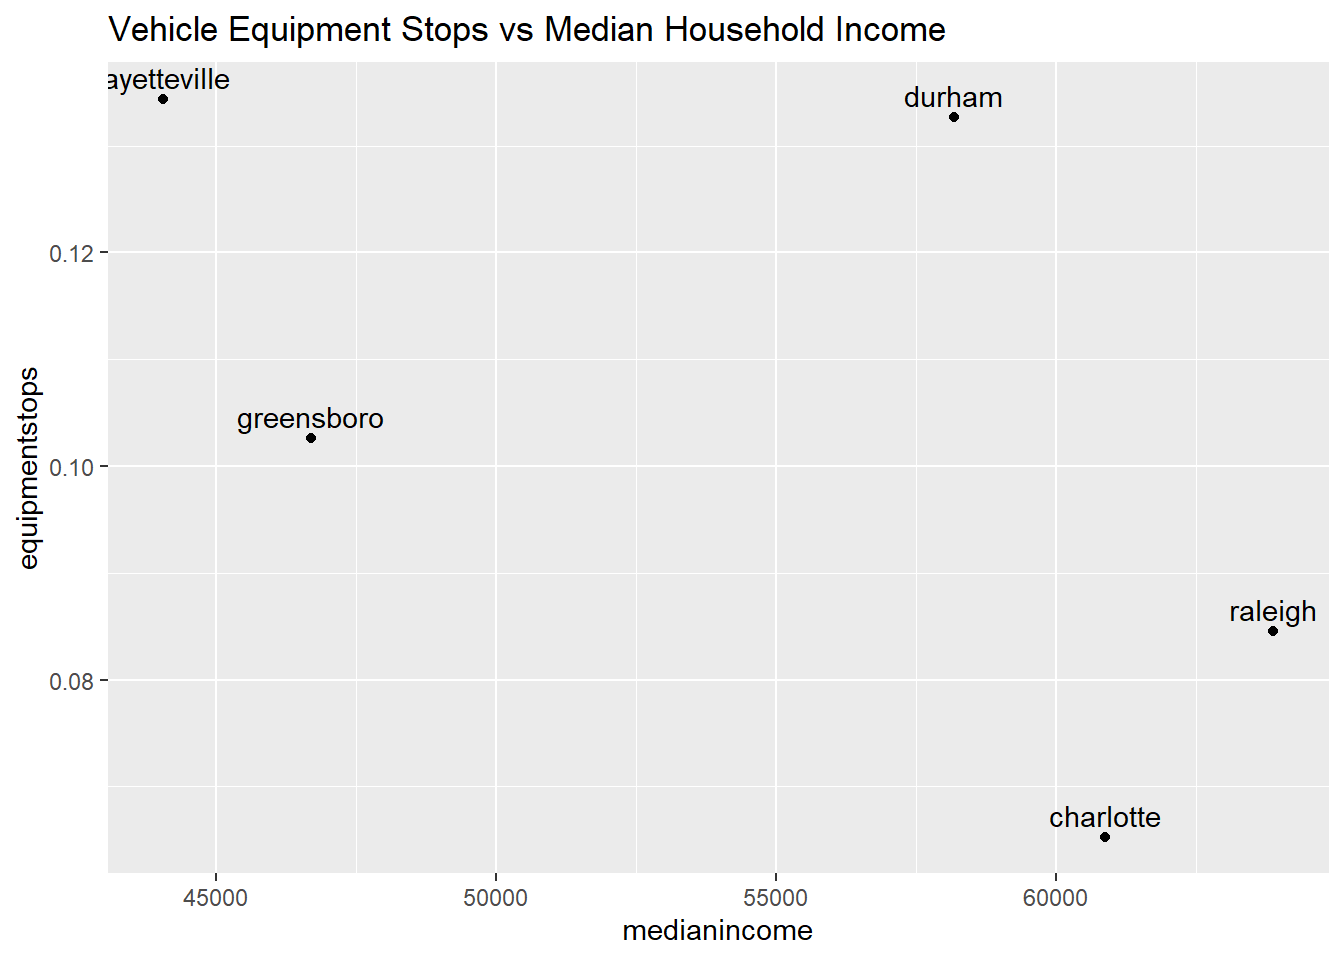
\includegraphics{bookdown-demo_files/figure-latex/unnamed-chunk-111-1.pdf}
We also look at vehicle regulatory stops against median household income, which also seems to be related to economically implications. Here we see a more clear trend excluding Fayetteville, that there is an increase in percentage stops with the increase of median income.

\hypertarget{modeling-the-probability-of-seach-given-stop}{%
\section{Modeling the Probability of Seach Given Stop}\label{modeling-the-probability-of-seach-given-stop}}

During night times when the sun is set, researchers speculate that stops are made by police officers without the acknowledgment of the racial identity of the driver. This should be the exact opposite for police officers during the day times. With the hope of identifying possible underlying racial discrimination with the available stop data, it has therefore been determined that for a specific region, the differences between the percentage of minority drivers within day times and night times could be used to detect such discrimination. The central idea is that, by observing the distribution of the difference values through the progression of time, we can gain a better understanding of the change of police behaviors with the transformation from day times to night times.

The calculation of the difference for this research project is set to be the daytime percentage of minority drivers (black) being stopped deducted by that of the night time percentage. A positive difference value indicates that if the police officer is able to identify the identity of the driver (i.e., under the day times), she or he has a higher percentage chance of stopping the minority driver. Whereas during the night times with a lack of sufficient light source, we assumed that the police officer was unable to identify the driver's race. Therefore, if there exists racial discrimination against minority drivers, we should expect to observe that a significant proportion of percentage differences should be positive. However, if the visualization shows an opposite distribution, then we have to conclude that the division of day time and night time has failed to capture the existence of racial discrimination.

\begin{Shaded}
\begin{Highlighting}[]
\NormalTok{SAN <-}\StringTok{ }\NormalTok{SAN }\OperatorTok
\StringTok{  }\NormalTok{dplyr}\OperatorTok{::}\KeywordTok{mutate}\NormalTok{(}\DataTypeTok{date2 =}\NormalTok{ lubridate}\OperatorTok{::}\KeywordTok{as_date}\NormalTok{(lubridate}\OperatorTok{::}\KeywordTok{ymd}\NormalTok{(}\KeywordTok{as.character}\NormalTok{(date)))) }

\NormalTok{SAN <-}\StringTok{ }\NormalTok{SAN }\OperatorTok\StringTok{ }\KeywordTok{mutate}\NormalTok{(}\DataTypeTok{date_time =} \KeywordTok{as.POSIXct}\NormalTok{(}\KeywordTok{paste}\NormalTok{(date, time), }\DataTypeTok{tz =} \StringTok{"America/Chicago"}\NormalTok{, }\DataTypeTok{format =} \StringTok{"%Y-%m-%d %H:%M:%OS"}\NormalTok{))}

\NormalTok{oursunriseset <-}\StringTok{ }\ControlFlowTok{function}\NormalTok{(latitude, longitude, date, }\DataTypeTok{direction =} \KeywordTok{c}\NormalTok{(}\StringTok{"sunrise"}\NormalTok{, }\StringTok{"sunset"}\NormalTok{)) \{}
\NormalTok{  date.lat.long <-}\StringTok{ }\KeywordTok{data.frame}\NormalTok{(}\DataTypeTok{date =}\NormalTok{ date, }\DataTypeTok{lat =}\NormalTok{ latitude, }\DataTypeTok{lon =}\NormalTok{ longitude)}
  \ControlFlowTok{if}\NormalTok{(direction }\OperatorTok{==}\StringTok{ "sunrise"}\NormalTok{)\{}
\NormalTok{    x <-}\StringTok{ }\KeywordTok{getSunlightTimes}\NormalTok{(}\DataTypeTok{data =}\NormalTok{ date.lat.long, }\DataTypeTok{keep=}\NormalTok{direction, }\DataTypeTok{tz=}\StringTok{"America/Chicago"}\NormalTok{)}\OperatorTok{$}\NormalTok{sunrise \}}\ControlFlowTok{else}\NormalTok{\{}
\NormalTok{    x <-}\StringTok{ }\KeywordTok{getSunlightTimes}\NormalTok{(}\DataTypeTok{data =}\NormalTok{ date.lat.long, }\DataTypeTok{keep=}\NormalTok{direction, }\DataTypeTok{tz=}\StringTok{"America/Chicago"}\NormalTok{)}\OperatorTok{$}\NormalTok{sunset  \}}
  \KeywordTok{return}\NormalTok{(x)}
\NormalTok{\}}

\NormalTok{sunrise <-}\StringTok{ }\KeywordTok{oursunriseset}\NormalTok{(}\FloatTok{29.4241}\NormalTok{, }\FloatTok{-98.4936}\NormalTok{, SAN}\OperatorTok{$}\NormalTok{date2, }\DataTypeTok{direction =} \StringTok{"sunrise"}\NormalTok{)}
\NormalTok{sunset <-}\StringTok{ }\KeywordTok{oursunriseset}\NormalTok{(}\FloatTok{29.4241}\NormalTok{, }\FloatTok{-98.4936}\NormalTok{, SAN}\OperatorTok{$}\NormalTok{date2, }\DataTypeTok{direction =} \StringTok{"sunset"}\NormalTok{)}

\NormalTok{SAN <-}\StringTok{ }\KeywordTok{cbind}\NormalTok{(SAN, sunrise, sunset)}

\NormalTok{SAN <-}\StringTok{ }\NormalTok{SAN }\OperatorTok
\KeywordTok{mutate}\NormalTok{(}\DataTypeTok{light =} \KeywordTok{ifelse}\NormalTok{(date_time }\OperatorTok{<}\StringTok{ }\NormalTok{sunrise, }\StringTok{"night"}\NormalTok{, }\KeywordTok{ifelse}\NormalTok{(date_time }\OperatorTok{>}\StringTok{ }\NormalTok{sunset, }\StringTok{"night"}\NormalTok{, }\StringTok{"day"}\NormalTok{)))}

\NormalTok{racial_perc <-}\StringTok{ }\ControlFlowTok{function}\NormalTok{(mon, yr, race)\{}
\NormalTok{  x1 <-}\StringTok{ }\KeywordTok{filter}\NormalTok{(SAN, light }\OperatorTok{==}\StringTok{ "day"}\NormalTok{, month }\OperatorTok{==}\StringTok{ }\NormalTok{mon, year }\OperatorTok{==}\StringTok{ }\NormalTok{yr)}
\NormalTok{  x1 <-}\StringTok{ }\KeywordTok{prop.table}\NormalTok{(}\KeywordTok{table}\NormalTok{(x1}\OperatorTok{$}\NormalTok{subject_race)) }
\NormalTok{  x1 <-}\StringTok{ }\KeywordTok{as.data.frame}\NormalTok{(x1)}
\NormalTok{  x1 <-}\StringTok{ }\KeywordTok{filter}\NormalTok{(x1, Var1 }\OperatorTok{==}\StringTok{ }\NormalTok{race)}\OperatorTok{$}\NormalTok{Freq}
  
\NormalTok{  x2 <-}\StringTok{ }\KeywordTok{filter}\NormalTok{(SAN,light }\OperatorTok{==}\StringTok{ "night"}\NormalTok{, month }\OperatorTok{==}\StringTok{ }\NormalTok{mon, year }\OperatorTok{==}\StringTok{ }\NormalTok{yr)}
\NormalTok{  x2 <-}\StringTok{ }\KeywordTok{prop.table}\NormalTok{(}\KeywordTok{table}\NormalTok{(x2}\OperatorTok{$}\NormalTok{subject_race)) }
\NormalTok{  x2 <-}\StringTok{ }\KeywordTok{as.data.frame}\NormalTok{(x2)}
\NormalTok{  x2 <-}\StringTok{ }\KeywordTok{filter}\NormalTok{(x2, Var1 }\OperatorTok{==}\StringTok{ }\NormalTok{race)}\OperatorTok{$}\NormalTok{Freq}
  
  \KeywordTok{return}\NormalTok{(x1}\OperatorTok{-}\NormalTok{x2)}
\NormalTok{\}}

\NormalTok{x <-}\StringTok{ }\KeywordTok{c}\NormalTok{()}
\NormalTok{y <-}\StringTok{ }\KeywordTok{c}\NormalTok{()}
\NormalTok{z <-}\StringTok{ }\KeywordTok{c}\NormalTok{()}
\ControlFlowTok{for}\NormalTok{ (i }\ControlFlowTok{in} \KeywordTok{seq}\NormalTok{(}\DecValTok{2012}\NormalTok{,}\DecValTok{2017}\NormalTok{))\{}
  \ControlFlowTok{for}\NormalTok{ (j }\ControlFlowTok{in} \KeywordTok{seq}\NormalTok{(}\DecValTok{1}\NormalTok{,}\DecValTok{12}\NormalTok{))\{}
\NormalTok{    diff <-}\StringTok{ }\KeywordTok{racial_perc}\NormalTok{(j,i,}\StringTok{"black"}\NormalTok{)}
\NormalTok{    x <-}\StringTok{ }\KeywordTok{c}\NormalTok{(x, diff)}
\NormalTok{    y <-}\StringTok{ }\KeywordTok{c}\NormalTok{(y,i)}
\NormalTok{    z <-}\StringTok{ }\KeywordTok{c}\NormalTok{(z,j)}
\NormalTok{  \}}
\NormalTok{\}}

\NormalTok{diff_data_SAN <-}\StringTok{ }\KeywordTok{as.data.frame}\NormalTok{(}\KeywordTok{cbind}\NormalTok{(x,y,z))}
\NormalTok{diff_data_SAN <-}\StringTok{ }\NormalTok{diff_data_SAN }\OperatorTok\StringTok{ }\KeywordTok{mutate}\NormalTok{(}\DataTypeTok{time =} \DecValTok{1}\OperatorTok{:}\KeywordTok{nrow}\NormalTok{(diff_data_SAN))}

\NormalTok{x <-}\StringTok{ }\KeywordTok{c}\NormalTok{()}
\NormalTok{y <-}\StringTok{ }\KeywordTok{c}\NormalTok{()}
\NormalTok{z <-}\StringTok{ }\KeywordTok{c}\NormalTok{()}
\ControlFlowTok{for}\NormalTok{ (i }\ControlFlowTok{in} \KeywordTok{seq}\NormalTok{(}\DecValTok{1}\NormalTok{,}\DecValTok{4}\NormalTok{))\{}
\NormalTok{  diff <-}\StringTok{ }\KeywordTok{racial_perc}\NormalTok{(i,}\StringTok{'2018'}\NormalTok{,}\StringTok{"black"}\NormalTok{)}
\NormalTok{  x <-}\StringTok{ }\KeywordTok{c}\NormalTok{(x, diff)}
\NormalTok{  z <-}\StringTok{ }\KeywordTok{c}\NormalTok{(}\DecValTok{1}\NormalTok{,}\DecValTok{2}\NormalTok{,}\DecValTok{3}\NormalTok{,}\DecValTok{4}\NormalTok{)}
\NormalTok{  y <-}\StringTok{ }\KeywordTok{c}\NormalTok{(}\DecValTok{2018}\NormalTok{, }\DecValTok{2018}\NormalTok{, }\DecValTok{2018}\NormalTok{, }\DecValTok{2018}\NormalTok{)}
\NormalTok{\}}

\NormalTok{n <-}\StringTok{ }\KeywordTok{nrow}\NormalTok{(diff_data_SAN)}
\NormalTok{diff_data_SAN2 <-}\StringTok{ }\KeywordTok{as.data.frame}\NormalTok{(}\KeywordTok{cbind}\NormalTok{(x,y,z))}
\NormalTok{diff_data_SAN2 <-}\StringTok{ }\NormalTok{diff_data_SAN2 }\OperatorTok\StringTok{ }\KeywordTok{mutate}\NormalTok{(}\DataTypeTok{time =}\NormalTok{ (n}\OperatorTok{+}\DecValTok{1}\NormalTok{)}\OperatorTok{:}\NormalTok{(n}\OperatorTok{+}\DecValTok{4}\NormalTok{))}
\NormalTok{diff_data_SAN <-}\StringTok{ }\KeywordTok{rbind}\NormalTok{(diff_data_SAN,diff_data_SAN2)}


\KeywordTok{ggplot}\NormalTok{(}\DataTypeTok{data =}\NormalTok{ diff_data_SAN) }\OperatorTok{+}\StringTok{ }
\StringTok{  }\KeywordTok{geom_point}\NormalTok{(}\DataTypeTok{mapping =} \KeywordTok{aes}\NormalTok{(}\DataTypeTok{x =}\NormalTok{ time, }\DataTypeTok{y =}\NormalTok{ x)) }\OperatorTok{+}
\StringTok{  }\KeywordTok{geom_hline}\NormalTok{(}\DataTypeTok{yintercept=}\DecValTok{0}\NormalTok{, }\DataTypeTok{linetype=}\StringTok{"dashed"}\NormalTok{, }\DataTypeTok{color =} \StringTok{"red"}\NormalTok{)}
\end{Highlighting}
\end{Shaded}

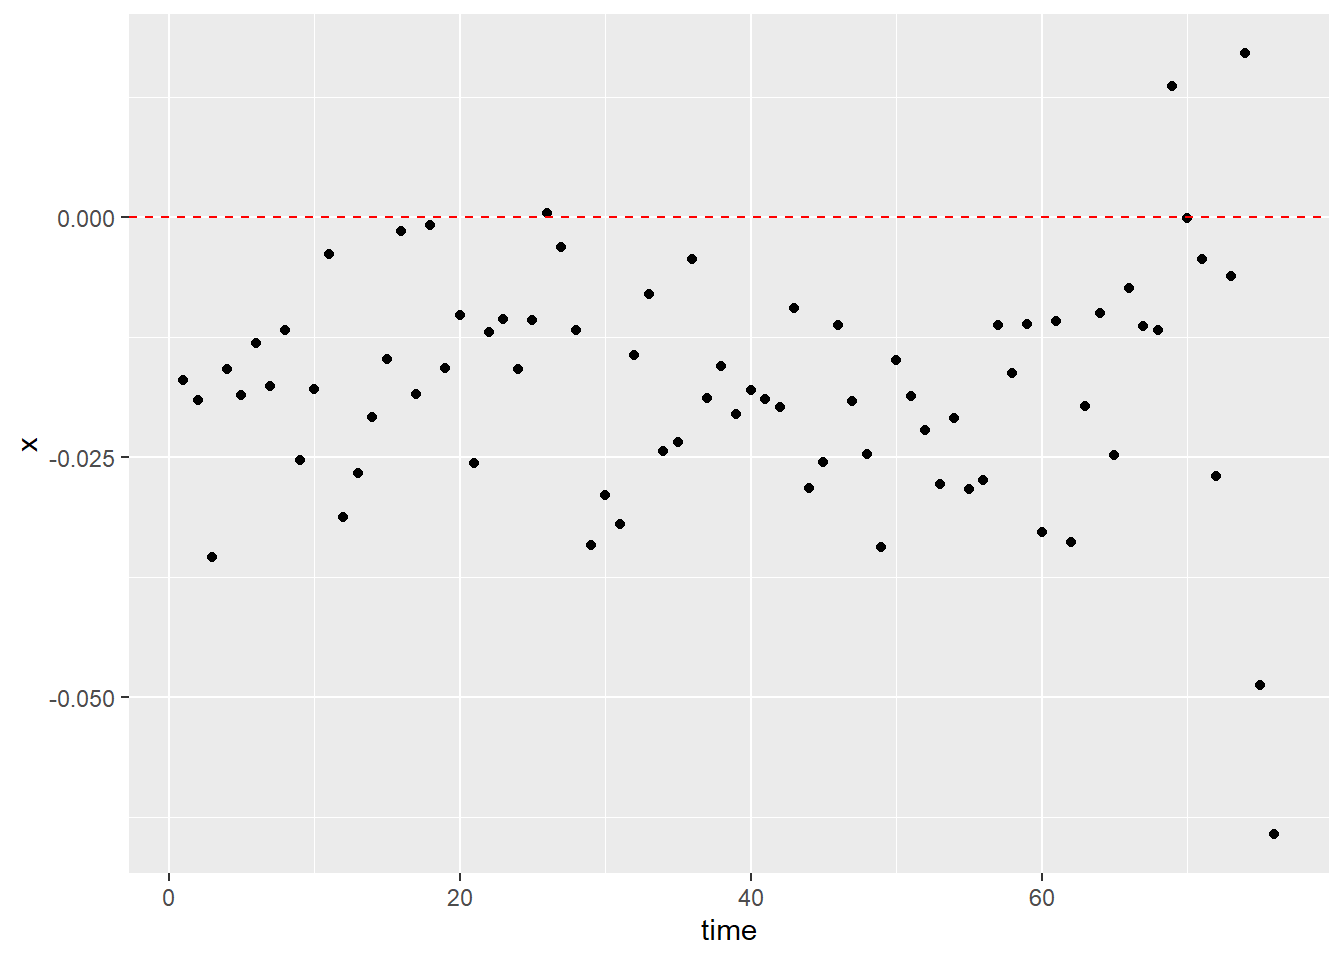
\includegraphics{bookdown-demo_files/figure-latex/unnamed-chunk-114-1.pdf}

The policing data used for the visualization is from Sanantonio, Texas, and the date is from January 2012 to April 2018. This data recorded a total number of 1,040,428 observations. Key variables are the date of the stop made and the race of the driver, and the corresponding sunrise and sunset time were calculated with each of the given dates. If the stop took place after the sunrise time and before the sunset time, it was set to be a stop made during the day time. Stops that took place outside of this range were set to be night time stops. Then for each day, the percentage of black drivers stopped during day and night was separately calculated and their difference was documented. Finally, the visualization of the key variables was a scatter plot with the horizontal axis as the progression of time and the vertical axis as the day time percentage deducted by night time percentage. For us to claim that the plot has successfully captured the possible existence of racial discrimination, we should expect to observe the majority of the points to be above the horizontal line at zero. However, the scatter plot demonstrates a trend contrary to our expectations. Most of the points fall under the horizontal line, which indicates that for the region of Sanantonio, black drivers on average were stopped at a lower percentage during day time than night time. Using this method and the given data, we have failed the attempt to prove that there has been racial discrimination against black drivers within the data.

One possible downfall of the aforementioned method is that it failed to acknowledge the possible difference in the distribution of driver populations between day time and night time. More specifically speaking, it is likely that for the region of Sanantonio, drivers who are on the road during night time and day time are two completely different population groups, and therefore, comparing the percentages of drivers stopped between these two possibly distinct population might be less meaningful. One possible improvement in the hope of alleviating population distinctions is the ``veil of darkness'' test, which limits to the stops made only one hour before and after the sunset time. This approach helps to reduce the possible distinction in the racial distribution of the night time and day time drivers. A similar set of procedures to the previous method was conducted, and a second scatter plot was produced. For the second time, the majority of the points are still below the horizontal line, which indicates that even if we have attempted to reduce the possible transformation of racial distribution, black drivers were mostly stopped at a higher percentage during night time relative to that of the day time. Therefore, the second plot has also failed to offer evidence for the existence of racial discrimination in the data for Sanantonio.

\begin{Shaded}
\begin{Highlighting}[]
\NormalTok{SAN2 <-}\StringTok{ }\NormalTok{SAN }\OperatorTok
\StringTok{  }\KeywordTok{filter}\NormalTok{(sunset}\DecValTok{-3600} \OperatorTok{<}\StringTok{ }\NormalTok{date_time }\OperatorTok{&}\StringTok{ }\NormalTok{sunset }\OperatorTok{+}\StringTok{ }\DecValTok{3600} \OperatorTok{>}\StringTok{ }\NormalTok{date_time)}

\NormalTok{racial_perc2 <-}\StringTok{ }\ControlFlowTok{function}\NormalTok{(mon, yr, race)\{}
\NormalTok{  x1 <-}\StringTok{ }\KeywordTok{filter}\NormalTok{(SAN2, light }\OperatorTok{==}\StringTok{ "day"}\NormalTok{, month }\OperatorTok{==}\StringTok{ }\NormalTok{mon, year }\OperatorTok{==}\StringTok{ }\NormalTok{yr)}
\NormalTok{  x1 <-}\StringTok{ }\KeywordTok{prop.table}\NormalTok{(}\KeywordTok{table}\NormalTok{(x1}\OperatorTok{$}\NormalTok{subject_race)) }
\NormalTok{  x1 <-}\StringTok{ }\KeywordTok{as.data.frame}\NormalTok{(x1)}
\NormalTok{  x1 <-}\StringTok{ }\KeywordTok{filter}\NormalTok{(x1, Var1 }\OperatorTok{==}\StringTok{ }\NormalTok{race)}\OperatorTok{$}\NormalTok{Freq}
  
\NormalTok{  x2 <-}\StringTok{ }\KeywordTok{filter}\NormalTok{(SAN2,light }\OperatorTok{==}\StringTok{ "night"}\NormalTok{, month }\OperatorTok{==}\StringTok{ }\NormalTok{mon, year }\OperatorTok{==}\StringTok{ }\NormalTok{yr)}
\NormalTok{  x2 <-}\StringTok{ }\KeywordTok{prop.table}\NormalTok{(}\KeywordTok{table}\NormalTok{(x2}\OperatorTok{$}\NormalTok{subject_race)) }
\NormalTok{  x2 <-}\StringTok{ }\KeywordTok{as.data.frame}\NormalTok{(x2)}
\NormalTok{  x2 <-}\StringTok{ }\KeywordTok{filter}\NormalTok{(x2, Var1 }\OperatorTok{==}\StringTok{ }\NormalTok{race)}\OperatorTok{$}\NormalTok{Freq}
  
  \KeywordTok{return}\NormalTok{(x1}\OperatorTok{-}\NormalTok{x2)}
\NormalTok{\}}

\NormalTok{x <-}\StringTok{ }\KeywordTok{c}\NormalTok{()}
\NormalTok{y <-}\StringTok{ }\KeywordTok{c}\NormalTok{()}
\NormalTok{z <-}\StringTok{ }\KeywordTok{c}\NormalTok{()}
\ControlFlowTok{for}\NormalTok{ (i }\ControlFlowTok{in} \KeywordTok{seq}\NormalTok{(}\DecValTok{2012}\NormalTok{,}\DecValTok{2017}\NormalTok{))\{}
  \ControlFlowTok{for}\NormalTok{ (j }\ControlFlowTok{in} \KeywordTok{seq}\NormalTok{(}\DecValTok{1}\NormalTok{,}\DecValTok{12}\NormalTok{))\{}
\NormalTok{    diff <-}\StringTok{ }\KeywordTok{racial_perc}\NormalTok{(j,i,}\StringTok{"black"}\NormalTok{)}
\NormalTok{    x <-}\StringTok{ }\KeywordTok{c}\NormalTok{(x, diff)}
\NormalTok{    y <-}\StringTok{ }\KeywordTok{c}\NormalTok{(y,i)}
\NormalTok{    z <-}\StringTok{ }\KeywordTok{c}\NormalTok{(z,j)}
\NormalTok{  \}}
\NormalTok{\}}

\NormalTok{diff_data_SAN <-}\StringTok{ }\KeywordTok{as.data.frame}\NormalTok{(}\KeywordTok{cbind}\NormalTok{(x,y,z))}
\NormalTok{diff_data_SAN <-}\StringTok{ }\NormalTok{diff_data_SAN }\OperatorTok\StringTok{ }\KeywordTok{mutate}\NormalTok{(}\DataTypeTok{time =} \DecValTok{1}\OperatorTok{:}\KeywordTok{nrow}\NormalTok{(diff_data_SAN))}

\NormalTok{x <-}\StringTok{ }\KeywordTok{c}\NormalTok{()}
\NormalTok{y <-}\StringTok{ }\KeywordTok{c}\NormalTok{()}
\NormalTok{z <-}\StringTok{ }\KeywordTok{c}\NormalTok{()}
\ControlFlowTok{for}\NormalTok{ (i }\ControlFlowTok{in} \KeywordTok{seq}\NormalTok{(}\DecValTok{1}\NormalTok{,}\DecValTok{4}\NormalTok{))\{}
\NormalTok{  diff <-}\StringTok{ }\KeywordTok{racial_perc2}\NormalTok{(i,}\StringTok{'2018'}\NormalTok{,}\StringTok{"black"}\NormalTok{)}
\NormalTok{  x <-}\StringTok{ }\KeywordTok{c}\NormalTok{(x, diff)}
\NormalTok{  z <-}\StringTok{ }\KeywordTok{c}\NormalTok{(}\DecValTok{1}\NormalTok{,}\DecValTok{2}\NormalTok{,}\DecValTok{3}\NormalTok{,}\DecValTok{4}\NormalTok{)}
\NormalTok{  y <-}\StringTok{ }\KeywordTok{c}\NormalTok{(}\DecValTok{2018}\NormalTok{, }\DecValTok{2018}\NormalTok{, }\DecValTok{2018}\NormalTok{, }\DecValTok{2018}\NormalTok{)}
\NormalTok{\}}

\NormalTok{n <-}\StringTok{ }\KeywordTok{nrow}\NormalTok{(diff_data_SAN)}
\NormalTok{diff_data_SAN2 <-}\StringTok{ }\KeywordTok{as.data.frame}\NormalTok{(}\KeywordTok{cbind}\NormalTok{(x,y,z))}
\NormalTok{diff_data_SAN2 <-}\StringTok{ }\NormalTok{diff_data_SAN2 }\OperatorTok\StringTok{ }\KeywordTok{mutate}\NormalTok{(}\DataTypeTok{time =}\NormalTok{ (n}\OperatorTok{+}\DecValTok{1}\NormalTok{)}\OperatorTok{:}\NormalTok{(n}\OperatorTok{+}\DecValTok{4}\NormalTok{))}
\NormalTok{diff_data_SAN <-}\StringTok{ }\KeywordTok{rbind}\NormalTok{(diff_data_SAN,diff_data_SAN2)}

\KeywordTok{ggplot}\NormalTok{(}\DataTypeTok{data =}\NormalTok{ diff_data_SAN) }\OperatorTok{+}\StringTok{ }
\StringTok{  }\KeywordTok{geom_point}\NormalTok{(}\DataTypeTok{mapping =} \KeywordTok{aes}\NormalTok{(}\DataTypeTok{x =}\NormalTok{ time, }\DataTypeTok{y =}\NormalTok{ x)) }\OperatorTok{+}
\StringTok{  }\KeywordTok{geom_hline}\NormalTok{(}\DataTypeTok{yintercept=}\DecValTok{0}\NormalTok{, }\DataTypeTok{linetype=}\StringTok{"dashed"}\NormalTok{, }\DataTypeTok{color =} \StringTok{"red"}\NormalTok{)}
\end{Highlighting}
\end{Shaded}

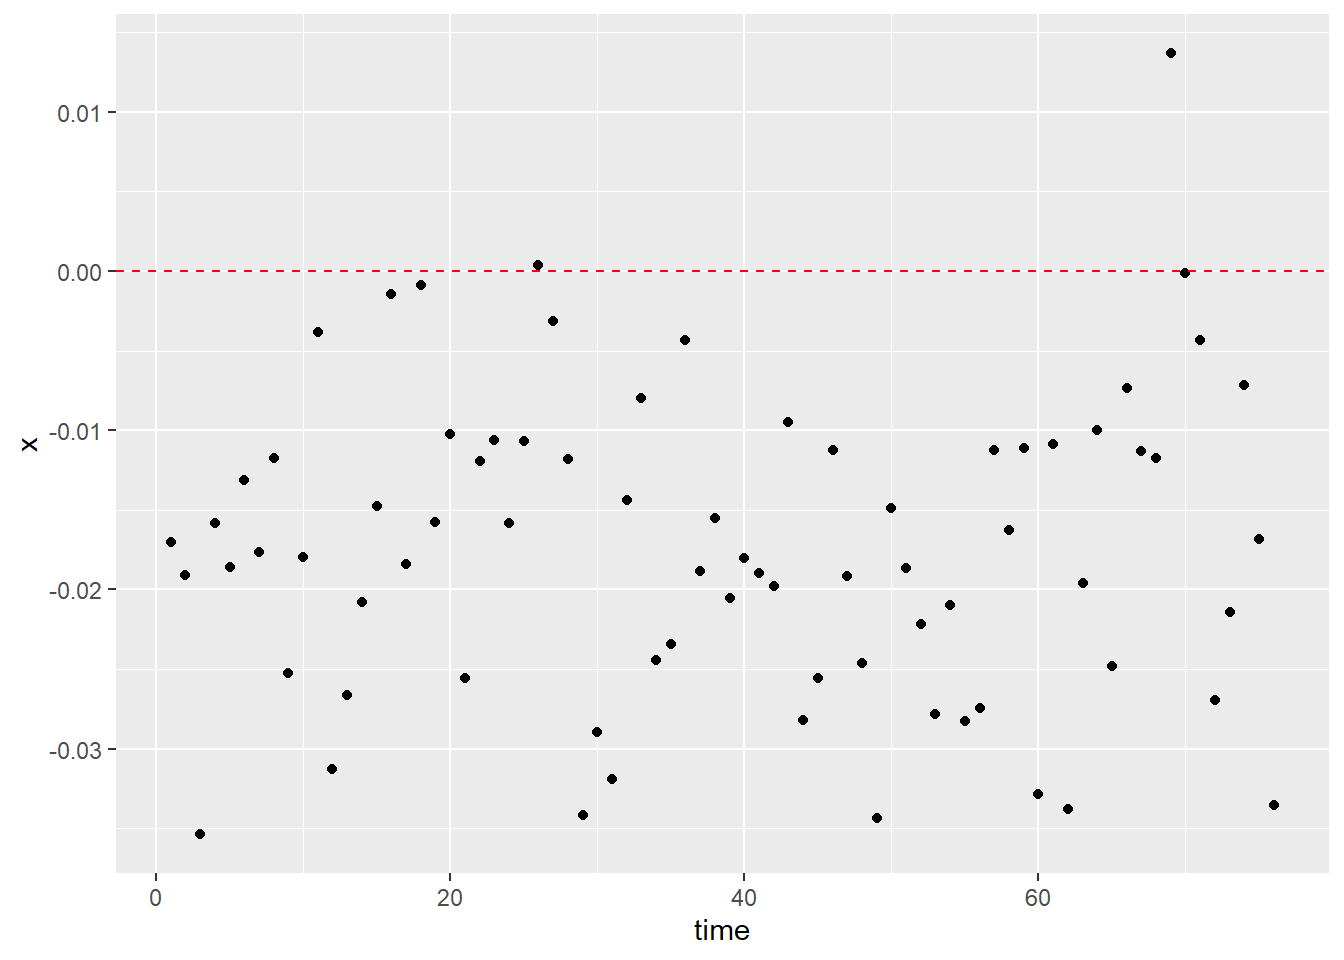
\includegraphics{bookdown-demo_files/figure-latex/unnamed-chunk-115-1.pdf}

\hypertarget{nationwide-logistic-regression}{%
\chapter{Nationwide Logistic Regression}\label{nationwide-logistic-regression}}

Here, we apply our logistic regression test to multiple cities or statewide datasets. The logistic regression in Charlotte, NC reveals distinct probabilities for black and white drivers as a function of age. The purposes behind applying the logistic regression to multiple cities is to observe differences in search conducted probabilities based on age and race and see if there is any interaction with age and race variables.

The logistic\_regression function takes in a dataset and name inputs. This function will run a logistic regression on the given datasets. Then, it takes the coefficients and added to a row of a data frame called, coefficient\_matrix. Each row coefficient\_matrix represents a different cities with their respective coefficients from the logistic regression.

\begin{Shaded}
\begin{Highlighting}[]
\NormalTok{coefficient_matrix <-}\StringTok{ }\KeywordTok{data.frame}\NormalTok{(}\StringTok{"intercept"}\NormalTok{ =}\StringTok{ }\KeywordTok{numeric}\NormalTok{(), }\StringTok{"subject_age"}\NormalTok{ =}\StringTok{ }\KeywordTok{numeric}\NormalTok{(), }\StringTok{"subject_race"}\NormalTok{ =}\StringTok{ }\KeywordTok{as.numeric}\NormalTok{(), }\StringTok{"subject_age.subject_race"}\NormalTok{ =}\StringTok{ }\KeywordTok{as.numeric}\NormalTok{(), }\StringTok{"dataset_name"}\NormalTok{ =}\StringTok{ }\KeywordTok{character}\NormalTok{())}

\NormalTok{logistic_regression <-}\StringTok{ }\ControlFlowTok{function}\NormalTok{(city_dataset, name)\{}
  
  \CommentTok{# run logistic regression}
\NormalTok{  fitlog <-}\StringTok{ }\KeywordTok{glm}\NormalTok{(}\DataTypeTok{formula =}\NormalTok{ search_binary }\OperatorTok{~}\StringTok{ }\NormalTok{subject_age}\OperatorTok{*}\NormalTok{subject_race, }\DataTypeTok{data =}\NormalTok{ city_dataset, }\DataTypeTok{family =}\NormalTok{ binomial, }\DataTypeTok{control =} \KeywordTok{list}\NormalTok{(}\DataTypeTok{maxit =} \DecValTok{50}\NormalTok{))}
  
  \CommentTok{# record logistic regression coefficients}
\NormalTok{  coefficient_row_vector =}\StringTok{ }\KeywordTok{t}\NormalTok{(fitlog}\OperatorTok{$}\NormalTok{coefficients)}

  \CommentTok{# row bind each coefficient and dataset tibble with the coefficent_matrix}
\NormalTok{  coefficient_matrix <<-}\StringTok{ }\KeywordTok{rbind}\NormalTok{(coefficient_matrix, }\KeywordTok{cbind.data.frame}\NormalTok{(}\KeywordTok{as.data.frame}\NormalTok{(coefficient_row_vector), name))}

\NormalTok{\}}

\KeywordTok{mapply}\NormalTok{(logistic_regression, datasets, datasets_of_interest) }

\NormalTok{coefficient_matrix}
\KeywordTok{colnames}\NormalTok{(coefficient_matrix) <-}\StringTok{ }\KeywordTok{c}\NormalTok{(}\StringTok{"intercept"}\NormalTok{, }\StringTok{"subject_age"}\NormalTok{, }\StringTok{"subject_raceW"}\NormalTok{, }\StringTok{"subject_age.subject_race"}\NormalTok{, }\StringTok{"datasetnames"}\NormalTok{)}
\end{Highlighting}
\end{Shaded}

Running the code above will output a dataframe in your local environment called coefficient matrix. We decided to write the dataframe as a csv file (``coeff\_matrix\_raw.csv'') so that we could resuse the coefficients.

\hypertarget{plotting-s-curves}{%
\section{Plotting S-curves}\label{plotting-s-curves}}

Plotting an S curve for 1 row of coefficients using the coefficient equation for black drivers
Ordering by all 50 states (found at \url{https://wallethub.com/edu/most-least-diverse-states-in-america/38262/\#methodology})

\begin{Shaded}
\begin{Highlighting}[]
\NormalTok{coeff_matrix <-}\StringTok{ }\KeywordTok{read.csv}\NormalTok{(}\StringTok{"coeff_matrix_raw.csv"}\NormalTok{)}
\NormalTok{matrix <-}\StringTok{ }\NormalTok{coeff_matrix[}\DecValTok{1}\NormalTok{,]}
\NormalTok{ages <-}\StringTok{ }\KeywordTok{seq}\NormalTok{(}\OperatorTok{-}\DecValTok{750}\NormalTok{,}\DecValTok{750}\NormalTok{,}\DecValTok{1}\NormalTok{)}
\NormalTok{coeff <-}\StringTok{ }\NormalTok{(matrix}\OperatorTok{$}\NormalTok{intercept) }\OperatorTok{+}\StringTok{ }\NormalTok{(matrix}\OperatorTok{$}\NormalTok{subject_age)}\OperatorTok{*}\NormalTok{ages}
\NormalTok{scurve <-}\StringTok{ }\KeywordTok{exp}\NormalTok{(coeff)}\OperatorTok{/}\NormalTok{(}\DecValTok{1}\OperatorTok{+}\KeywordTok{exp}\NormalTok{(coeff))}
\NormalTok{plot.data <-}\StringTok{ }\KeywordTok{data.frame}\NormalTok{(}\DataTypeTok{subject_age=}\NormalTok{scurve, }\DataTypeTok{age=}\NormalTok{ages)}
\NormalTok{plot.data <-}\StringTok{ }\KeywordTok{gather}\NormalTok{(plot.data, }\DataTypeTok{key=}\NormalTok{group, }\DataTypeTok{value=}\NormalTok{prob, subject_age)}
\KeywordTok{ggplot}\NormalTok{(plot.data, }\KeywordTok{aes}\NormalTok{(}\DataTypeTok{x=}\NormalTok{age, }\DataTypeTok{y=}\NormalTok{prob, }\DataTypeTok{color=}\NormalTok{group)) }\OperatorTok{+}\StringTok{ }\KeywordTok{geom_line}\NormalTok{(}\DataTypeTok{lwd=}\DecValTok{2}\NormalTok{) }\OperatorTok{+}\StringTok{ }
\KeywordTok{labs}\NormalTok{(}\DataTypeTok{x=}\StringTok{"age"}\NormalTok{, }\DataTypeTok{y=}\StringTok{"P(outcome)"}\NormalTok{, }\DataTypeTok{title=}\StringTok{"Probability of being search conducted"}\NormalTok{)}
\end{Highlighting}
\end{Shaded}

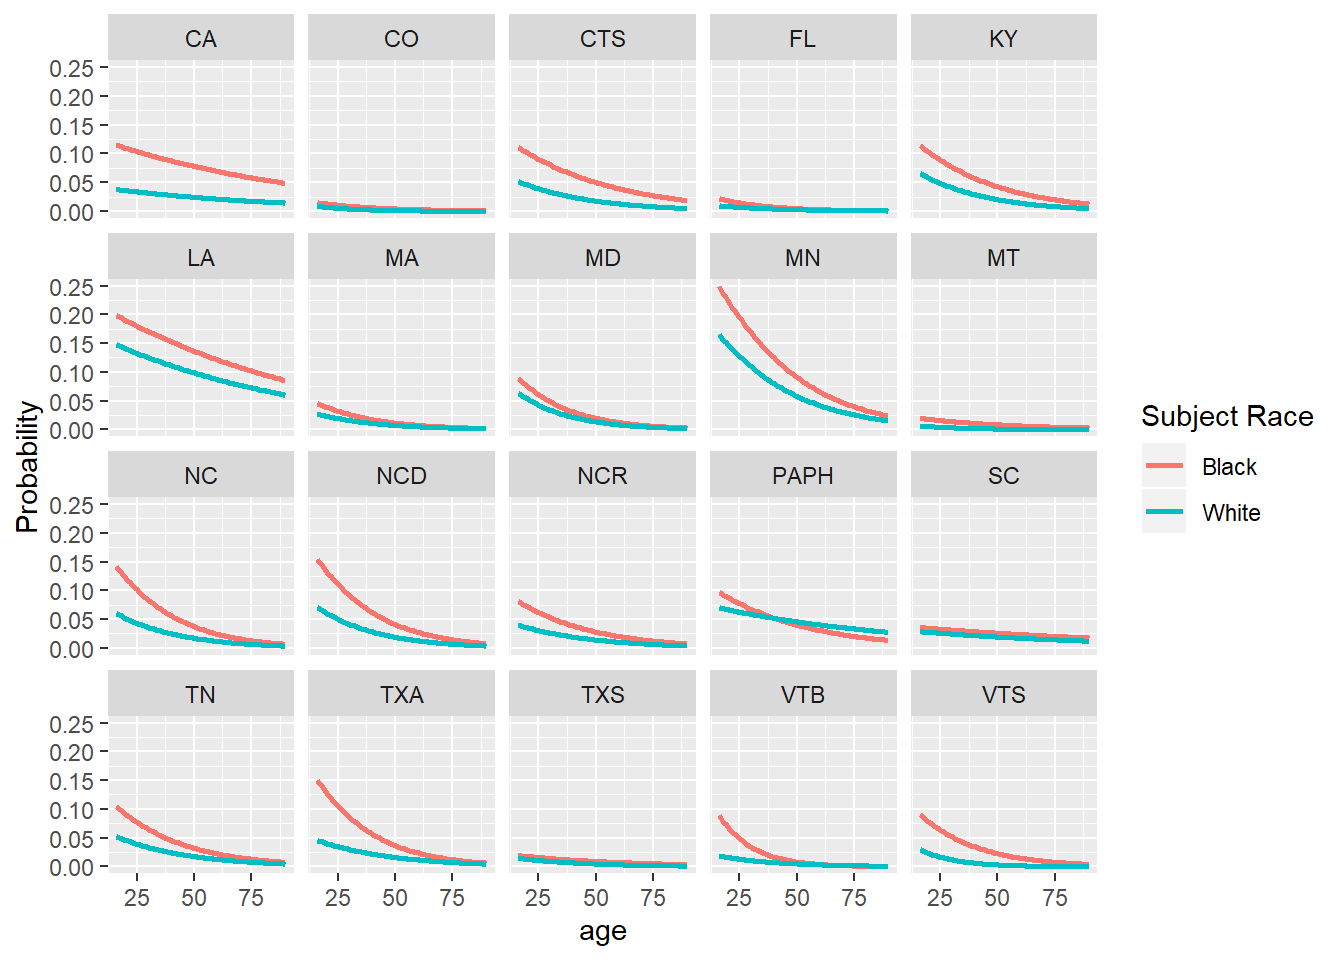
\includegraphics{bookdown-demo_files/figure-latex/unnamed-chunk-40-1.pdf}

\begin{Shaded}
\begin{Highlighting}[]
\CommentTok{# looking at an appropriate age range of 16-90}
\NormalTok{ages <-}\StringTok{ }\KeywordTok{seq}\NormalTok{(}\DecValTok{16}\NormalTok{,}\DecValTok{90}\NormalTok{,}\DecValTok{1}\NormalTok{)}
\NormalTok{coeff <-}\StringTok{ }\NormalTok{(matrix}\OperatorTok{$}\NormalTok{intercept) }\OperatorTok{+}\StringTok{ }\NormalTok{(matrix}\OperatorTok{$}\NormalTok{subject_age)}\OperatorTok{*}\NormalTok{ages}
\NormalTok{scurve <-}\StringTok{ }\KeywordTok{exp}\NormalTok{(coeff)}\OperatorTok{/}\NormalTok{(}\DecValTok{1}\OperatorTok{+}\KeywordTok{exp}\NormalTok{(coeff))}
\NormalTok{plot.data <-}\StringTok{ }\KeywordTok{data.frame}\NormalTok{(}\DataTypeTok{subject_age_black=}\NormalTok{scurve, }\DataTypeTok{age=}\NormalTok{ages)}
\NormalTok{plot.data <-}\StringTok{ }\KeywordTok{gather}\NormalTok{(plot.data, }\DataTypeTok{key=}\NormalTok{group, }\DataTypeTok{value=}\NormalTok{prob, subject_age_black)}
\KeywordTok{ggplot}\NormalTok{(plot.data, }\KeywordTok{aes}\NormalTok{(}\DataTypeTok{x=}\NormalTok{age, }\DataTypeTok{y=}\NormalTok{prob, }\DataTypeTok{color=}\NormalTok{group)) }\OperatorTok{+}
\StringTok{  }\KeywordTok{geom_line}\NormalTok{(}\DataTypeTok{lwd=}\DecValTok{2}\NormalTok{) }\OperatorTok{+}\StringTok{ }
\StringTok{  }\KeywordTok{labs}\NormalTok{(}\DataTypeTok{x=}\StringTok{"age"}\NormalTok{, }\DataTypeTok{y=}\StringTok{"P(outcome)"}\NormalTok{, }\DataTypeTok{title=}\StringTok{"Probability of being search conducted"}\NormalTok{)}
\end{Highlighting}
\end{Shaded}

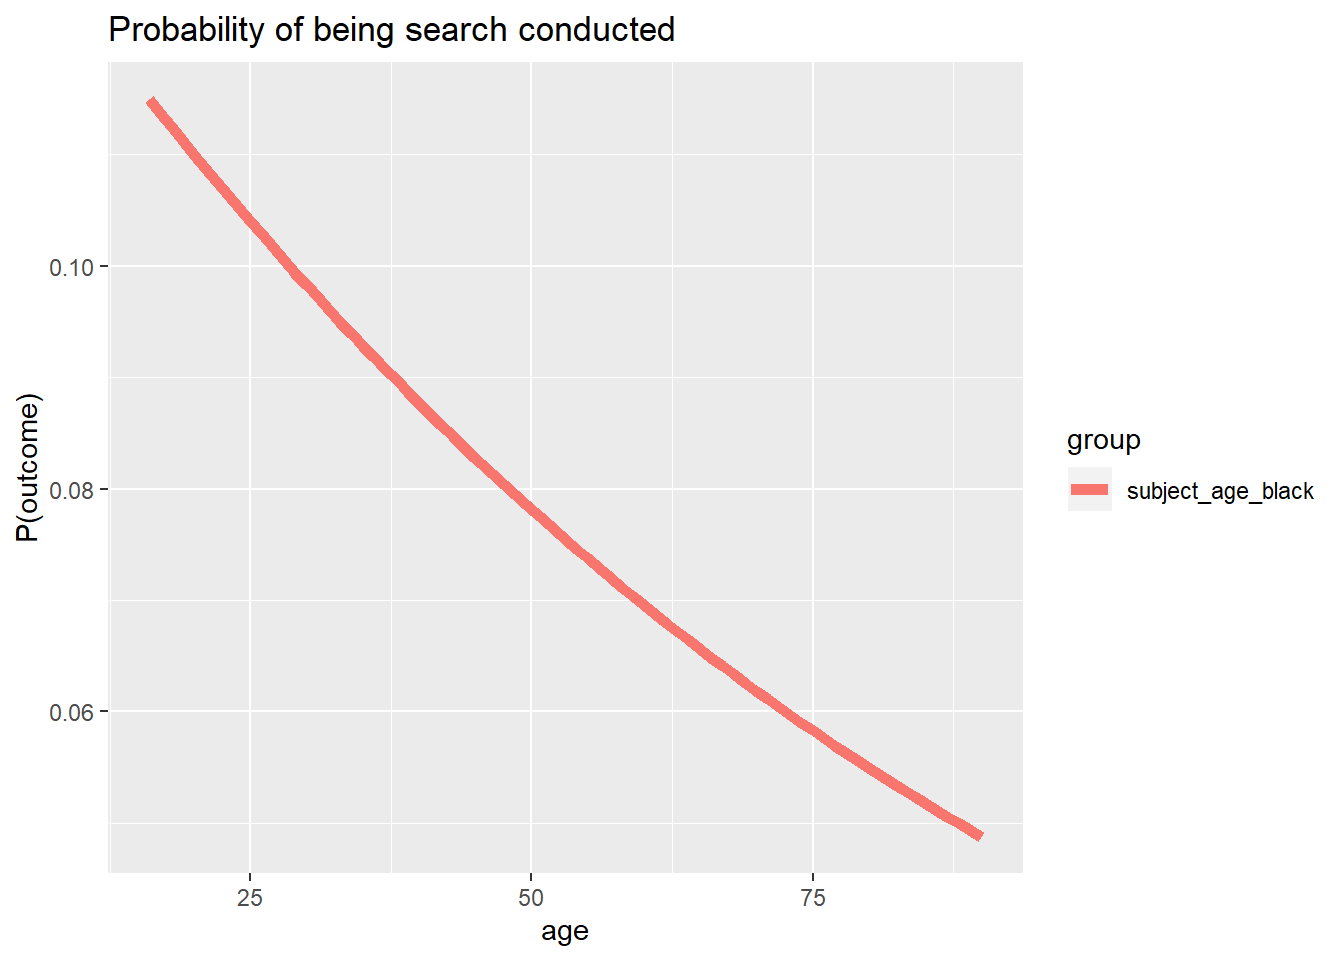
\includegraphics{bookdown-demo_files/figure-latex/unnamed-chunk-40-2.pdf}
This displays the same equation but for white drivers.

\begin{Shaded}
\begin{Highlighting}[]
\NormalTok{ages <-}\StringTok{ }\KeywordTok{seq}\NormalTok{(}\OperatorTok{-}\DecValTok{750}\NormalTok{,}\DecValTok{750}\NormalTok{,}\DecValTok{1}\NormalTok{)}
\NormalTok{coeff <-}\StringTok{ }\NormalTok{((matrix}\OperatorTok{$}\NormalTok{intercept) }\OperatorTok{+}\StringTok{ }\NormalTok{(matrix}\OperatorTok{$}\NormalTok{subject_race)) }\OperatorTok{+}\StringTok{ }
\StringTok{  }\NormalTok{(matrix}\OperatorTok{$}\NormalTok{subject_age }\OperatorTok{+}\StringTok{ }\NormalTok{matrix}\OperatorTok{$}\NormalTok{subject_age.subject_race)}\OperatorTok{*}\NormalTok{ages}
\NormalTok{scurve <-}\StringTok{ }\KeywordTok{exp}\NormalTok{(coeff)}\OperatorTok{/}\NormalTok{(}\DecValTok{1}\OperatorTok{+}\KeywordTok{exp}\NormalTok{(coeff))}
\NormalTok{plot.data <-}\StringTok{ }\KeywordTok{data.frame}\NormalTok{(}\DataTypeTok{subject_age_white=}\NormalTok{scurve, }\DataTypeTok{age=}\NormalTok{ages)}
\NormalTok{plot.data <-}\StringTok{ }\KeywordTok{gather}\NormalTok{(plot.data, }\DataTypeTok{key=}\NormalTok{group, }\DataTypeTok{value=}\NormalTok{prob, subject_age_white)}
\KeywordTok{ggplot}\NormalTok{(plot.data, }\KeywordTok{aes}\NormalTok{(}\DataTypeTok{x=}\NormalTok{age, }\DataTypeTok{y=}\NormalTok{prob, }\DataTypeTok{color=}\NormalTok{group)) }\OperatorTok{+}\StringTok{ }
\StringTok{  }\KeywordTok{geom_line}\NormalTok{(}\DataTypeTok{lwd=}\DecValTok{2}\NormalTok{) }\OperatorTok{+}\StringTok{ }
\StringTok{  }\KeywordTok{labs}\NormalTok{(}\DataTypeTok{x=}\StringTok{"age"}\NormalTok{, }\DataTypeTok{y=}\StringTok{"P(outcome)"}\NormalTok{, }\DataTypeTok{title=}\StringTok{"Probability of being search conducted"}\NormalTok{)}
\end{Highlighting}
\end{Shaded}

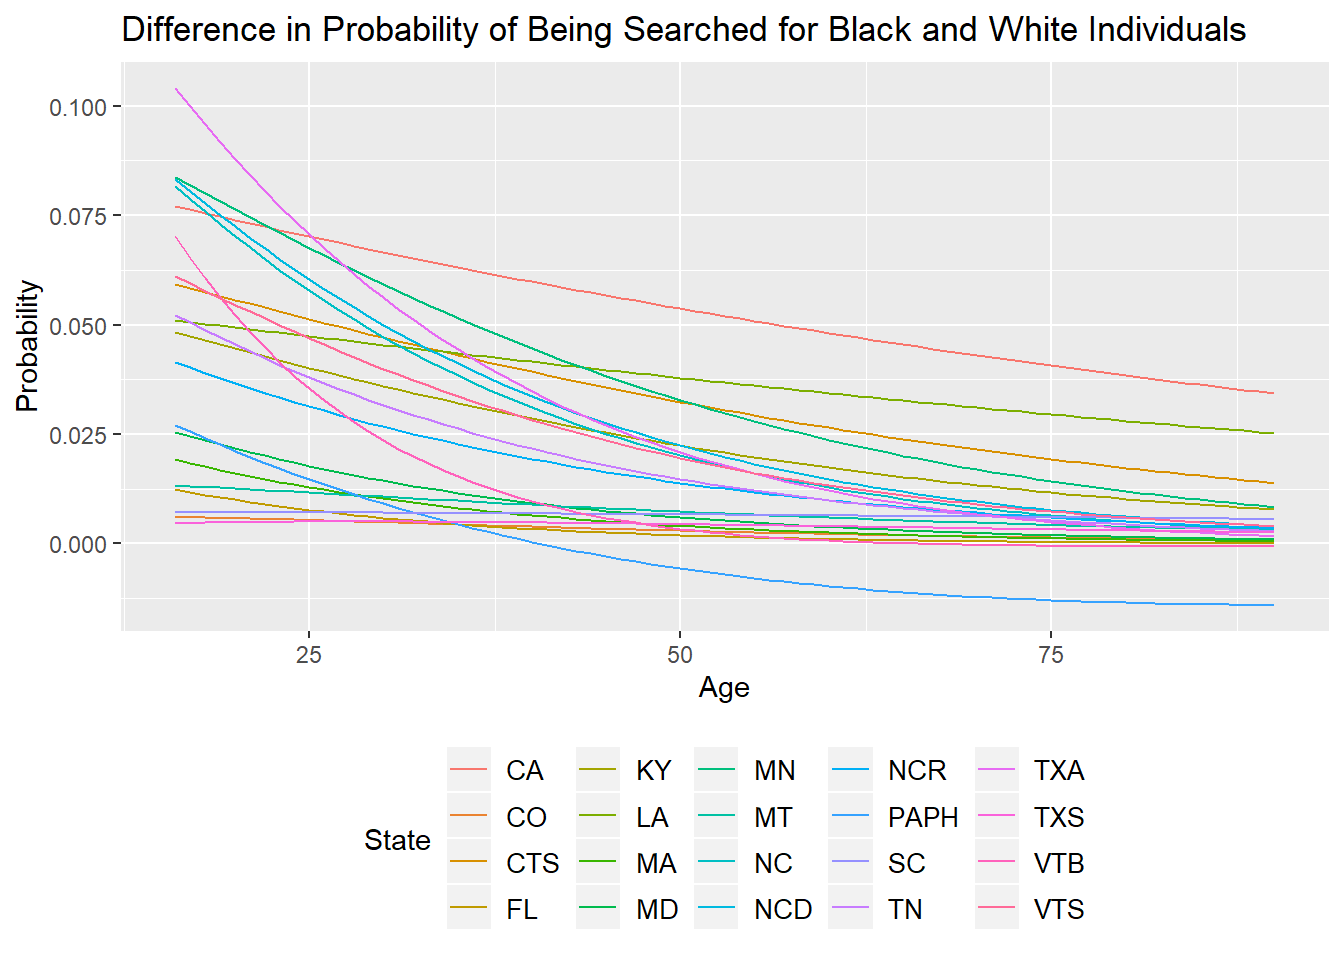
\includegraphics{bookdown-demo_files/figure-latex/unnamed-chunk-41-1.pdf}

\begin{Shaded}
\begin{Highlighting}[]
\NormalTok{ages <-}\StringTok{ }\KeywordTok{seq}\NormalTok{(}\DecValTok{16}\NormalTok{,}\DecValTok{90}\NormalTok{,}\DecValTok{1}\NormalTok{)}
\NormalTok{coeff <-}\StringTok{ }\NormalTok{((matrix}\OperatorTok{$}\NormalTok{intercept) }\OperatorTok{+}\StringTok{ }\NormalTok{(matrix}\OperatorTok{$}\NormalTok{subject_race)) }\OperatorTok{+}\StringTok{ }
\StringTok{  }\NormalTok{(matrix}\OperatorTok{$}\NormalTok{subject_age }\OperatorTok{+}\StringTok{ }\NormalTok{matrix}\OperatorTok{$}\NormalTok{subject_age.subject_race)}\OperatorTok{*}\NormalTok{ages}
\NormalTok{scurve <-}\StringTok{ }\KeywordTok{exp}\NormalTok{(coeff)}\OperatorTok{/}\NormalTok{(}\DecValTok{1}\OperatorTok{+}\KeywordTok{exp}\NormalTok{(coeff))}
\NormalTok{plot.data <-}\StringTok{ }\KeywordTok{data.frame}\NormalTok{(}\DataTypeTok{subject_age_white=}\NormalTok{scurve, }\DataTypeTok{age=}\NormalTok{ages)}
\NormalTok{plot.data <-}\StringTok{ }\KeywordTok{gather}\NormalTok{(plot.data, }\DataTypeTok{key=}\NormalTok{group, }\DataTypeTok{value=}\NormalTok{prob, subject_age_white)}
\KeywordTok{ggplot}\NormalTok{(plot.data, }\KeywordTok{aes}\NormalTok{(}\DataTypeTok{x=}\NormalTok{age, }\DataTypeTok{y=}\NormalTok{prob, }\DataTypeTok{color=}\NormalTok{group)) }\OperatorTok{+}
\StringTok{  }\KeywordTok{geom_line}\NormalTok{(}\DataTypeTok{lwd=}\DecValTok{2}\NormalTok{) }\OperatorTok{+}\StringTok{ }
\StringTok{  }\KeywordTok{labs}\NormalTok{(}\DataTypeTok{x=}\StringTok{"age"}\NormalTok{, }\DataTypeTok{y=}\StringTok{"P(outcome)"}\NormalTok{, }\DataTypeTok{title=}\StringTok{"Probability of being search conducted"}\NormalTok{)}
\end{Highlighting}
\end{Shaded}

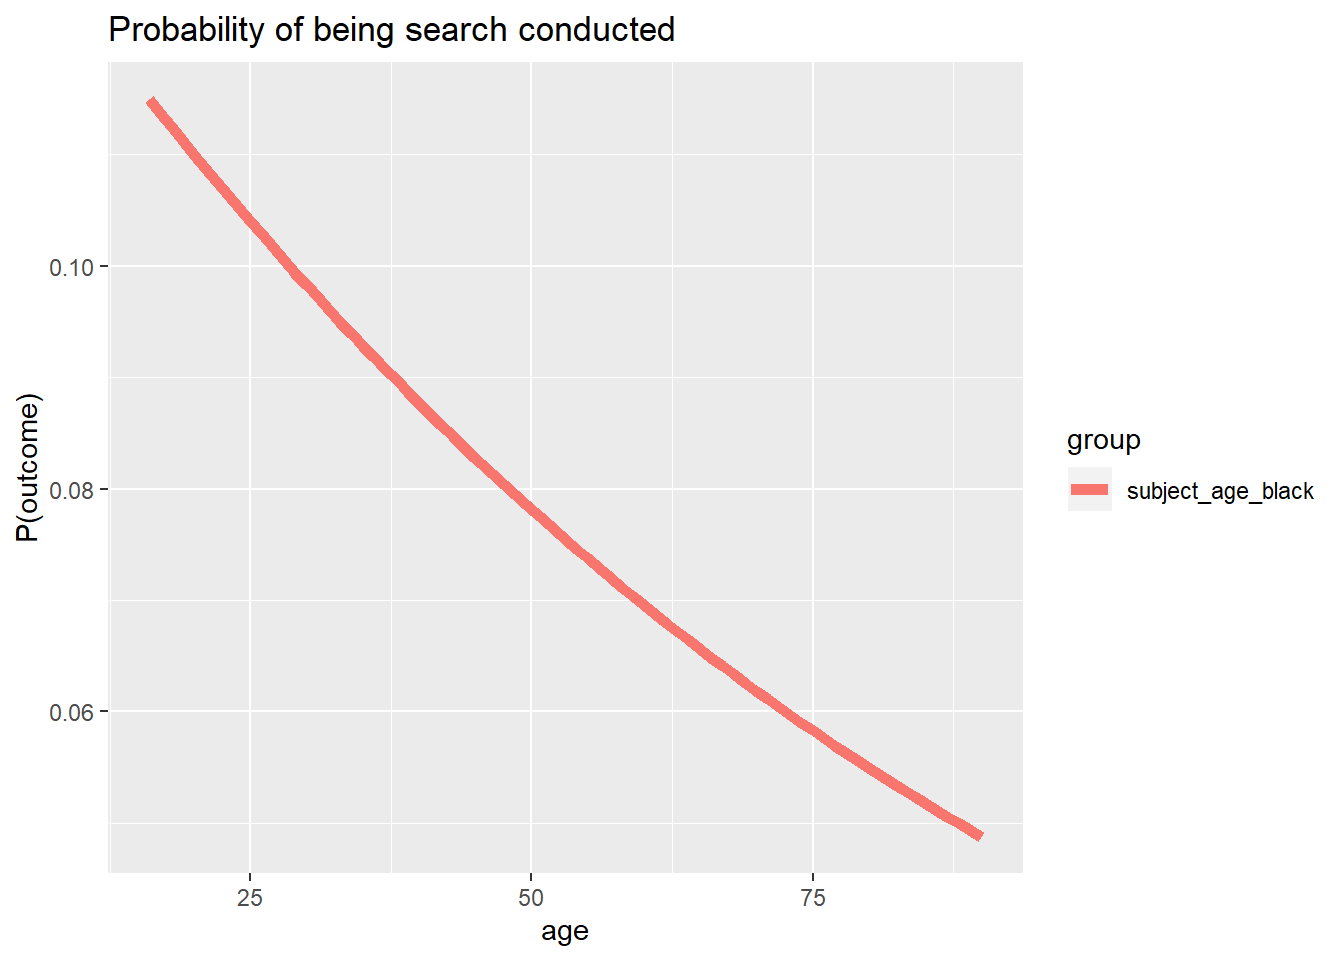
\includegraphics{bookdown-demo_files/figure-latex/unnamed-chunk-41-2.pdf}
Plotting both curves (black and white drivers) for each state

\begin{Shaded}
\begin{Highlighting}[]
\ControlFlowTok{for}\NormalTok{ (num }\ControlFlowTok{in} \DecValTok{1}\OperatorTok{:}\DecValTok{22}\NormalTok{)\{}
\NormalTok{matrix <-}\StringTok{ }\NormalTok{coeff_matrix[num,]}
\NormalTok{ages <-}\StringTok{ }\KeywordTok{seq}\NormalTok{(}\DecValTok{16}\NormalTok{,}\DecValTok{90}\NormalTok{,}\DecValTok{1}\NormalTok{)}
\NormalTok{coeff_b <-}\StringTok{ }\NormalTok{(matrix}\OperatorTok{$}\NormalTok{intercept) }\OperatorTok{+}\StringTok{ }\NormalTok{(matrix}\OperatorTok{$}\NormalTok{subject_age)}\OperatorTok{*}\NormalTok{ages}
\NormalTok{coeff_w <-}\StringTok{ }\NormalTok{((matrix}\OperatorTok{$}\NormalTok{intercept) }\OperatorTok{+}\StringTok{ }\NormalTok{(matrix}\OperatorTok{$}\NormalTok{subject_race)) }\OperatorTok{+}\StringTok{ }
\StringTok{  }\NormalTok{(matrix}\OperatorTok{$}\NormalTok{subject_age }\OperatorTok{+}\StringTok{ }\NormalTok{matrix}\OperatorTok{$}\NormalTok{subject_age.subject_race)}\OperatorTok{*}\NormalTok{ages}
\NormalTok{scurve_b <-}\StringTok{ }\KeywordTok{exp}\NormalTok{(coeff_b)}\OperatorTok{/}\NormalTok{(}\DecValTok{1}\OperatorTok{+}\KeywordTok{exp}\NormalTok{(coeff_b))}
\NormalTok{scurve_w <-}\StringTok{ }\KeywordTok{exp}\NormalTok{(coeff_w)}\OperatorTok{/}\NormalTok{(}\DecValTok{1}\OperatorTok{+}\KeywordTok{exp}\NormalTok{(coeff_w))}
\NormalTok{plot_b <-}\StringTok{ }\KeywordTok{data.frame}\NormalTok{(}\DataTypeTok{prob=}\NormalTok{scurve_b, }\DataTypeTok{age=}\NormalTok{ages, }\DataTypeTok{state =}\NormalTok{ matrix}\OperatorTok{$}\NormalTok{state_abbreviation)}
\NormalTok{plot_w <-}\StringTok{ }\KeywordTok{data.frame}\NormalTok{(}\DataTypeTok{prob=}\NormalTok{scurve_w, }\DataTypeTok{age=}\NormalTok{ages, }\DataTypeTok{state =}\NormalTok{ matrix}\OperatorTok{$}\NormalTok{state_abbreviation)}
\KeywordTok{print}\NormalTok{(}\KeywordTok{ggplot}\NormalTok{(plot_b, }\KeywordTok{aes}\NormalTok{(}\DataTypeTok{x=}\NormalTok{age, }\DataTypeTok{y=}\NormalTok{prob, }\DataTypeTok{color=}\StringTok{"blue"}\NormalTok{)) }\OperatorTok{+}
\KeywordTok{geom_line}\NormalTok{(}\DataTypeTok{lwd=}\FloatTok{1.5}\NormalTok{) }\OperatorTok{+}\StringTok{ }\KeywordTok{geom_line}\NormalTok{(plot_w, }
                               \DataTypeTok{mapping =} \KeywordTok{aes}\NormalTok{(}\DataTypeTok{x=}\NormalTok{age, }\DataTypeTok{y=}\NormalTok{prob, }\DataTypeTok{color=}\StringTok{"red"}\NormalTok{), }\DataTypeTok{lwd=}\FloatTok{1.5}\NormalTok{) }\OperatorTok{+}\StringTok{ }
\StringTok{  }\KeywordTok{ggtitle}\NormalTok{(matrix}\OperatorTok{$}\NormalTok{state_abbreviation))\}}
\end{Highlighting}
\end{Shaded}

Compiling all states onto one graph for black drivers. The results show that generally, the probably of being searched is lower as an individual gets older for both races. Notice the one positive trend (maybe a mistake in the dataset that we could share with Stanford?)

\begin{Shaded}
\begin{Highlighting}[]
\NormalTok{my_plot <-}\StringTok{ }\KeywordTok{ggplot}\NormalTok{()}
\ControlFlowTok{for}\NormalTok{ (num }\ControlFlowTok{in} \DecValTok{1}\OperatorTok{:}\DecValTok{22}\NormalTok{)\{}
\NormalTok{matrix <-}\StringTok{ }\NormalTok{coeff_matrix[num,]}
\NormalTok{ages <-}\StringTok{ }\KeywordTok{seq}\NormalTok{(}\DecValTok{16}\NormalTok{,}\DecValTok{90}\NormalTok{,}\DecValTok{1}\NormalTok{)}
\NormalTok{coeff <-}\StringTok{ }\NormalTok{(matrix}\OperatorTok{$}\NormalTok{intercept) }\OperatorTok{+}\StringTok{ }\NormalTok{(matrix}\OperatorTok{$}\NormalTok{subject_age)}\OperatorTok{*}\NormalTok{ages}
\NormalTok{scurve <-}\StringTok{ }\KeywordTok{exp}\NormalTok{(coeff)}\OperatorTok{/}\NormalTok{(}\DecValTok{1}\OperatorTok{+}\KeywordTok{exp}\NormalTok{(coeff))}
\NormalTok{plot <-}\StringTok{ }\KeywordTok{data.frame}\NormalTok{(}\DataTypeTok{Probability=}\NormalTok{scurve, }\DataTypeTok{Age=}\NormalTok{ages, }\DataTypeTok{State =}\NormalTok{ matrix}\OperatorTok{$}\NormalTok{state_abbreviation)}
\NormalTok{my_plot <-}\StringTok{ }\NormalTok{my_plot }\OperatorTok{+}\StringTok{ }\KeywordTok{geom_line}\NormalTok{(plot, }\DataTypeTok{mapping =} \KeywordTok{aes}\NormalTok{(}\DataTypeTok{x=}\NormalTok{Age, }\DataTypeTok{y=}\NormalTok{Probability, }\DataTypeTok{color=}\NormalTok{State))\}}
\NormalTok{my_plot }\OperatorTok{+}\StringTok{ }\KeywordTok{theme}\NormalTok{(}\DataTypeTok{legend.text =} \KeywordTok{element_text}\NormalTok{(}\DataTypeTok{size =} \DecValTok{10}\NormalTok{))}
\end{Highlighting}
\end{Shaded}

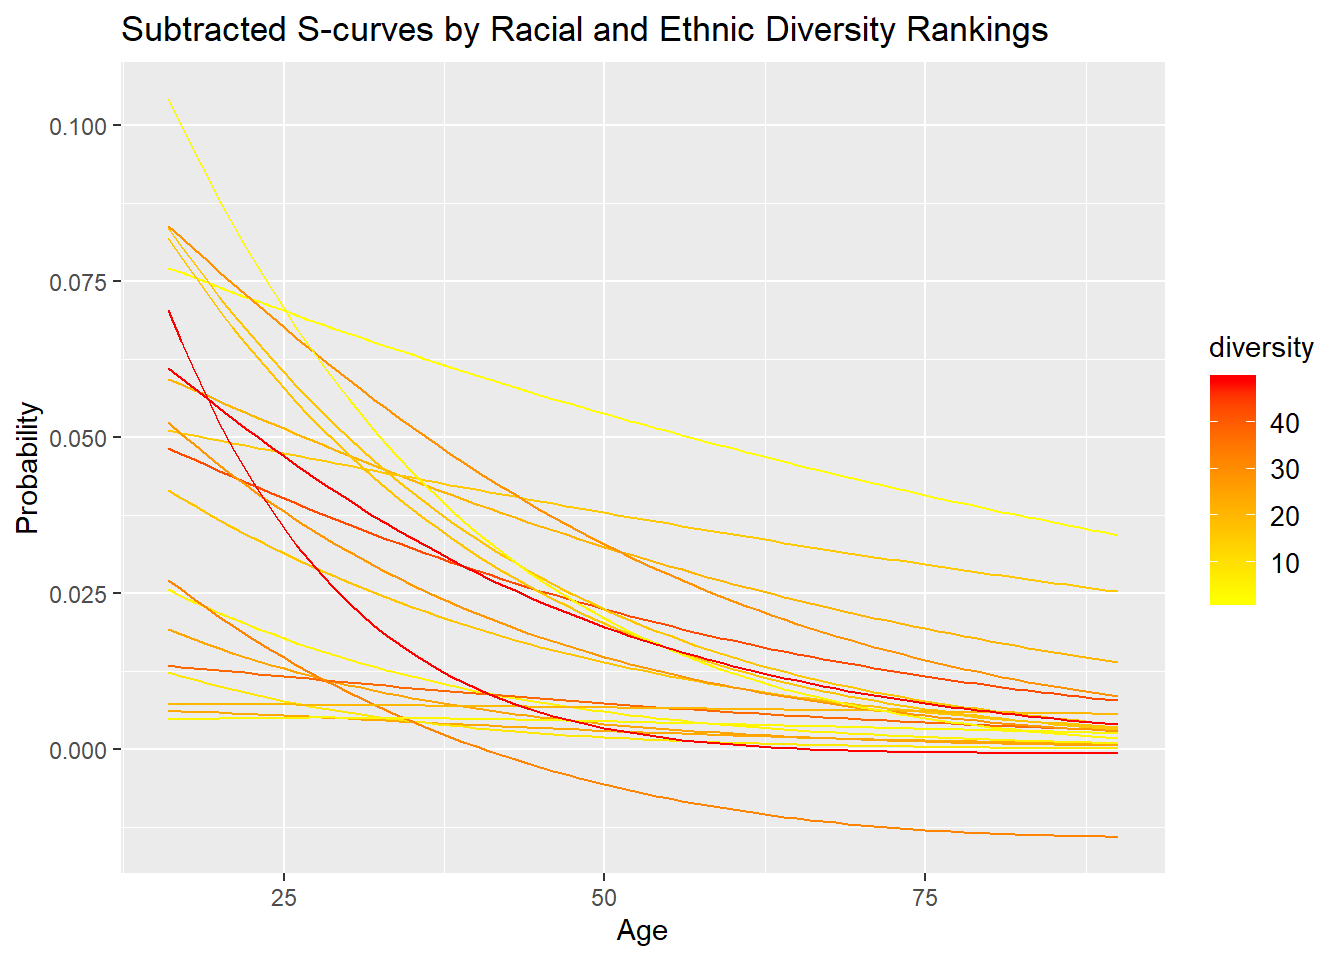
\includegraphics{bookdown-demo_files/figure-latex/unnamed-chunk-43-1.pdf}
We then subtracted the s-curve results for black and white drivers with each curve being grouped by the political party the state voted for in the 2016 election. The results indicate that in the majority of states, the probability of being searched is greater for black individuals than for white individuals of every age.

\begin{Shaded}
\begin{Highlighting}[]
\NormalTok{my_plot <-}\StringTok{ }\KeywordTok{ggplot}\NormalTok{()}
\ControlFlowTok{for}\NormalTok{ (num }\ControlFlowTok{in} \DecValTok{1}\OperatorTok{:}\DecValTok{22}\NormalTok{)\{}
\NormalTok{matrix <-}\StringTok{ }\NormalTok{coeff_matrix[num,]}
\NormalTok{ages <-}\StringTok{ }\KeywordTok{seq}\NormalTok{(}\DecValTok{16}\NormalTok{,}\DecValTok{90}\NormalTok{,}\DecValTok{1}\NormalTok{)}
\NormalTok{coeff <-}\StringTok{ }\NormalTok{(matrix}\OperatorTok{$}\NormalTok{intercept) }\OperatorTok{+}\StringTok{ }\NormalTok{(matrix}\OperatorTok{$}\NormalTok{subject_age)}\OperatorTok{*}\NormalTok{ages}
\NormalTok{coeff2 <-}\StringTok{ }\NormalTok{((matrix}\OperatorTok{$}\NormalTok{intercept) }\OperatorTok{+}\StringTok{ }\NormalTok{(matrix}\OperatorTok{$}\NormalTok{subject_race)) }\OperatorTok{+}\StringTok{ }
\StringTok{  }\NormalTok{(matrix}\OperatorTok{$}\NormalTok{subject_age }\OperatorTok{+}\StringTok{ }\NormalTok{matrix}\OperatorTok{$}\NormalTok{subject_age.subject_race)}\OperatorTok{*}\NormalTok{ages}
\NormalTok{scurve1 <-}\StringTok{ }\KeywordTok{exp}\NormalTok{(coeff)}\OperatorTok{/}\NormalTok{(}\DecValTok{1}\OperatorTok{+}\KeywordTok{exp}\NormalTok{(coeff))}
\NormalTok{scurve2 <-}\StringTok{ }\KeywordTok{exp}\NormalTok{(coeff2)}\OperatorTok{/}\NormalTok{(}\DecValTok{1}\OperatorTok{+}\KeywordTok{exp}\NormalTok{(coeff2))}
\NormalTok{scurve <-}\StringTok{ }\NormalTok{scurve1 }\OperatorTok{-}\StringTok{ }\NormalTok{scurve2}
\NormalTok{plot <-}\StringTok{ }\KeywordTok{data.frame}\NormalTok{(}\DataTypeTok{Probability=}\NormalTok{scurve, }\DataTypeTok{Age=}\NormalTok{ages, }
                   \DataTypeTok{State =}\NormalTok{ matrix}\OperatorTok{$}\NormalTok{state_abbreviation, }\DataTypeTok{makeup =}\NormalTok{ matrix}\OperatorTok{$}\NormalTok{state_politics)}
\NormalTok{my_plot <-}\StringTok{ }\NormalTok{my_plot }\OperatorTok{+}\StringTok{ }\KeywordTok{geom_line}\NormalTok{(plot, }\DataTypeTok{mapping =} \KeywordTok{aes}\NormalTok{(}\DataTypeTok{x=}\NormalTok{Age, }\DataTypeTok{y=}\NormalTok{Probability, }\DataTypeTok{color=}\NormalTok{makeup))\}}
\NormalTok{my_plot }\OperatorTok{+}\StringTok{ }\KeywordTok{scale_color_manual}\NormalTok{(}\DataTypeTok{values =} \KeywordTok{c}\NormalTok{(}\StringTok{"blue"}\NormalTok{, }\StringTok{"red"}\NormalTok{)) }\OperatorTok{+}\StringTok{ }
\StringTok{  }\KeywordTok{theme}\NormalTok{(}\DataTypeTok{legend.text =} \KeywordTok{element_text}\NormalTok{(}\DataTypeTok{size =} \DecValTok{10}\NormalTok{)) }\OperatorTok{+}\StringTok{ }
\StringTok{  }\KeywordTok{ggtitle}\NormalTok{(}\StringTok{"Subtracted S-curves by blue or red state"}\NormalTok{)}
\end{Highlighting}
\end{Shaded}

We then continued by grouping by various forms of diversity found at \url{https://wallethub.com/edu/most-least-diverse-states-in-america/38262/\#methodology}). This was done on a sliding scale for the ranks.

\begin{Shaded}
\begin{Highlighting}[]
\NormalTok{my_plot <-}\StringTok{ }\KeywordTok{ggplot}\NormalTok{()}
\ControlFlowTok{for}\NormalTok{ (num }\ControlFlowTok{in} \DecValTok{1}\OperatorTok{:}\DecValTok{22}\NormalTok{)\{}
\NormalTok{matrix <-}\StringTok{ }\NormalTok{coeff_matrix[num,]}
\NormalTok{ages <-}\StringTok{ }\KeywordTok{seq}\NormalTok{(}\DecValTok{16}\NormalTok{,}\DecValTok{90}\NormalTok{,}\DecValTok{1}\NormalTok{)}
\NormalTok{coeff <-}\StringTok{ }\NormalTok{(matrix}\OperatorTok{$}\NormalTok{intercept) }\OperatorTok{+}\StringTok{ }\NormalTok{(matrix}\OperatorTok{$}\NormalTok{subject_age)}\OperatorTok{*}\NormalTok{ages}
\NormalTok{coeff2 <-}\StringTok{ }\NormalTok{((matrix}\OperatorTok{$}\NormalTok{intercept) }\OperatorTok{+}\StringTok{ }\NormalTok{(matrix}\OperatorTok{$}\NormalTok{subject_race)) }\OperatorTok{+}\StringTok{ }
\StringTok{  }\NormalTok{(matrix}\OperatorTok{$}\NormalTok{subject_age }\OperatorTok{+}\StringTok{ }\NormalTok{matrix}\OperatorTok{$}\NormalTok{subject_age.subject_race)}\OperatorTok{*}\NormalTok{ages}
\NormalTok{scurve1 <-}\StringTok{ }\KeywordTok{exp}\NormalTok{(coeff)}\OperatorTok{/}\NormalTok{(}\DecValTok{1}\OperatorTok{+}\KeywordTok{exp}\NormalTok{(coeff))}
\NormalTok{scurve2 <-}\StringTok{ }\KeywordTok{exp}\NormalTok{(coeff2)}\OperatorTok{/}\NormalTok{(}\DecValTok{1}\OperatorTok{+}\KeywordTok{exp}\NormalTok{(coeff2))}
\NormalTok{scurve <-}\StringTok{ }\NormalTok{scurve1 }\OperatorTok{-}\StringTok{ }\NormalTok{scurve2}
\NormalTok{plot <-}\StringTok{ }\KeywordTok{data.frame}\NormalTok{(}\DataTypeTok{Probability=}\NormalTok{scurve, }\DataTypeTok{Age=}\NormalTok{ages, }
                   \DataTypeTok{State =}\NormalTok{ matrix}\OperatorTok{$}\NormalTok{state_abbreviation, }\DataTypeTok{makeup =}\NormalTok{ matrix}\OperatorTok{$}\NormalTok{state_politics, }
                   \DataTypeTok{diversity =}\NormalTok{ matrix}\OperatorTok{$}\NormalTok{racial_and_ethnic)}
\NormalTok{my_plot <-}\StringTok{ }\NormalTok{my_plot }\OperatorTok{+}\StringTok{ }\KeywordTok{geom_line}\NormalTok{(plot, }\DataTypeTok{mapping =} \KeywordTok{aes}\NormalTok{(}\DataTypeTok{x=}\NormalTok{Age, }\DataTypeTok{y=}\NormalTok{Probability, }\DataTypeTok{color=}\NormalTok{diversity))\}}
\NormalTok{my_plot }\OperatorTok{+}\StringTok{ }\KeywordTok{scale_color_gradient}\NormalTok{(}\DataTypeTok{low =} \StringTok{"green"}\NormalTok{, }\DataTypeTok{high =} \StringTok{"red"}\NormalTok{) }\OperatorTok{+}\StringTok{ }
\StringTok{  }\KeywordTok{theme}\NormalTok{(}\DataTypeTok{legend.text =} \KeywordTok{element_text}\NormalTok{(}\DataTypeTok{size =} \DecValTok{10}\NormalTok{)) }\OperatorTok{+}\StringTok{ }
\StringTok{  }\KeywordTok{ggtitle}\NormalTok{(}\StringTok{"Subtracted S-curves by racial and ethnic diversity"}\NormalTok{)}
\end{Highlighting}
\end{Shaded}

Notice that none seem to have any trend. Further work can be done to analyze other variables to group over.

\hypertarget{veil-of-darkness-nationwide}{%
\section{Veil of Darkness Nationwide}\label{veil-of-darkness-nationwide}}

Running a veil of darkness logistic regression follows a similar process as using race and age as variables to predict a search being conducted. This time, we add a light binary variable

First we want to get the relevant datasets. This time, we splice out different datasets as those are empty
Here we apply the relevant\_datasets function to get the character string. Then, we can use base R splicing to remove empty datasets.

This code block defines the function, query\_data, which calls the SQL command to retrieve the datasets with their speficied variables. Lastly, it will append each dataset to a list called datasets.

At last, the previous four functions will be called in the clean\_data function. Clean\_data does two main things:
1) make search conducted into a binary datatype
2) add night and day variables to our dataset
Notice how this is very similar to the previous clean\_data function only this time we add a add\_night\_day function

\begin{Shaded}
\begin{Highlighting}[]
\NormalTok{clean_data <-}\StringTok{ }\ControlFlowTok{function}\NormalTok{(i)\{}
\NormalTok{  city_dataset <-}\StringTok{ }\NormalTok{datasets[[i]] }\OperatorTok\StringTok{ }\KeywordTok{drop_na}\NormalTok{()}
  
  \CommentTok{# first add light and day variables}
\NormalTok{  tmp_lat <-}\StringTok{ }\NormalTok{coordinates[[i]][}\DecValTok{1}\NormalTok{]}
\NormalTok{  tmp_long <-}\StringTok{ }\NormalTok{coordinates[[i]][}\DecValTok{2}\NormalTok{]}
\NormalTok{  time_zone <-}\StringTok{ }\NormalTok{lutz}\OperatorTok{::}\KeywordTok{tz_lookup_coords}\NormalTok{(tmp_lat, tmp_long, }\DataTypeTok{warn =}\NormalTok{ F)}
\NormalTok{  city_dataset <-}\StringTok{ }\KeywordTok{add_night_day}\NormalTok{(city_dataset, time_zone, tmp_lat, tmp_long)}

  \CommentTok{# clean data}
  \ControlFlowTok{if}\NormalTok{ (}\KeywordTok{typeof}\NormalTok{(city_dataset}\OperatorTok{$}\NormalTok{search_conducted) }\OperatorTok{==}\StringTok{ "character"}\NormalTok{)\{}

\NormalTok{    city_dataset <-}\StringTok{ }\NormalTok{city_dataset }\OperatorTok
\StringTok{      }\KeywordTok{filter}\NormalTok{(subject_race }\OperatorTok{==}\StringTok{ "black"} \OperatorTok{|}\StringTok{ }\NormalTok{subject_race }\OperatorTok{==}\StringTok{ "white"}\NormalTok{) }\OperatorTok
\StringTok{      }\KeywordTok{mutate}\NormalTok{(}\DataTypeTok{search_conducted =} \KeywordTok{case_when}\NormalTok{(search_conducted }\OperatorTok{==}\StringTok{ "TRUE"} \OperatorTok{~}\StringTok{ }\DecValTok{1}\NormalTok{,}
\NormalTok{                                       search_conducted }\OperatorTok{==}\StringTok{ "FALSE"} \OperatorTok{~}\StringTok{ }\DecValTok{0}\NormalTok{))}
\NormalTok{  \} }\ControlFlowTok{else}\NormalTok{ \{}
    \CommentTok{# some datasets have search_conducted as already a dbl}
\NormalTok{    city_dataset <-}\StringTok{ }\NormalTok{city_dataset }\OperatorTok
\StringTok{    }\KeywordTok{filter}\NormalTok{(subject_race }\OperatorTok{==}\StringTok{ "black"} \OperatorTok{|}\StringTok{ }\NormalTok{subject_race }\OperatorTok{==}\StringTok{ "white"}\NormalTok{) }\OperatorTok
\StringTok{    }\KeywordTok{mutate}\NormalTok{(}\DataTypeTok{search_conducted =}\NormalTok{ search_conducted)}
\NormalTok{  \}}

\NormalTok{  city_dataset <-}\StringTok{ }\NormalTok{city_dataset }\OperatorTok
\StringTok{    }\KeywordTok{mutate}\NormalTok{(}\DataTypeTok{subject_race =} \KeywordTok{as.factor}\NormalTok{(}\KeywordTok{case_when}\NormalTok{(subject_race }\OperatorTok{==}\StringTok{ "white"}\OperatorTok{~}\StringTok{"W"}\NormalTok{, subject_race}\OperatorTok{==}\StringTok{"black"}\OperatorTok{~}\StringTok{"B"}\NormalTok{)))}

 
  \KeywordTok{return}\NormalTok{(city_dataset)}
\NormalTok{\}}

\NormalTok{datasets <-}\StringTok{ }\KeywordTok{lapply}\NormalTok{(}\KeywordTok{seq}\NormalTok{(datasets), clean_data)}
\end{Highlighting}
\end{Shaded}

fix\_ages quickly sets any ages to a dbl data type

\begin{Shaded}
\begin{Highlighting}[]
\NormalTok{fix_ages <-}\StringTok{ }\ControlFlowTok{function}\NormalTok{(city_dataset)\{}
\NormalTok{  city_dataset <-}\StringTok{ }\NormalTok{city_dataset }\OperatorTok\StringTok{ }\KeywordTok{mutate}\NormalTok{(}\DataTypeTok{subject_age =} \KeywordTok{as.numeric}\NormalTok{(subject_age)) }
  \KeywordTok{return}\NormalTok{(city_dataset)}
\NormalTok{\}}

\NormalTok{datasets<-}\StringTok{ }\KeywordTok{lapply}\NormalTok{(datasets, fix_ages)}
\end{Highlighting}
\end{Shaded}

Since we are analyzing multiple outputs from a logistic regression, we need a way to store those outputs. We decided to takes the coefficients from each logistic regression and make a dataframe out of them.

\begin{Shaded}
\begin{Highlighting}[]
\NormalTok{coefficient_matrix <-}\StringTok{ }\KeywordTok{data.frame}\NormalTok{(}\StringTok{"intercept"}\NormalTok{ =}\StringTok{ }\KeywordTok{numeric}\NormalTok{(), }\StringTok{"subject_raceW"}\NormalTok{ =}\StringTok{ }\KeywordTok{as.numeric}\NormalTok{(), }\StringTok{"subject_age"}\NormalTok{ =}\StringTok{ }\KeywordTok{as.numeric}\NormalTok{(), }\StringTok{"is_dark"}\NormalTok{ =}\StringTok{ }\KeywordTok{as.numeric}\NormalTok{(), }\StringTok{"subject_raceW:subject_age"}\NormalTok{ =}\StringTok{ }\KeywordTok{as.numeric}\NormalTok{(), }\StringTok{"subject_raceW:is_dark"}\NormalTok{ =}\StringTok{ }\KeywordTok{as.numeric}\NormalTok{(), }\StringTok{"subject_age:is_dark"}\NormalTok{ =}\StringTok{ }\KeywordTok{as.numeric}\NormalTok{(), }\StringTok{"subject_raceW:subject_age:is_dark"}\NormalTok{ =}\StringTok{ }\KeywordTok{as.numeric}\NormalTok{(), }\StringTok{"dataset_name"}\NormalTok{ =}\StringTok{ }\KeywordTok{character}\NormalTok{())}

\KeywordTok{mapply}\NormalTok{(logistic_regression, datasets, datasets_of_interest) }

\KeywordTok{colnames}\NormalTok{(coefficient_matrix) <-}\StringTok{ }\KeywordTok{c}\NormalTok{(}\StringTok{"intercept"}\NormalTok{, }\StringTok{"subject_raceW"}\NormalTok{, }\StringTok{"subject_age"}\NormalTok{, }\StringTok{"is_dark"}\NormalTok{, }\StringTok{"subject_raceW:subject_age"}\NormalTok{, }\StringTok{"subject_raceW:is_dark"}\NormalTok{, }\StringTok{"subject_age:is_dark"}\NormalTok{, }\StringTok{"datasetnames"}\NormalTok{)}
\end{Highlighting}
\end{Shaded}

Now that we have the coefficient\_matrix we can select certain coefficients to plot the s-curve for white and black people along with day and night. There are four s-curve we want to plot: Black driver in the day, Black and night, white and day, and White and night. Thus, we'll make a dataframe for each scenario and then row bind all of them.

\begin{Shaded}
\begin{Highlighting}[]
\NormalTok{plot_all <-}\StringTok{ }\ControlFlowTok{function}\NormalTok{(i)\{}
\NormalTok{  matrix <-}\StringTok{ }\NormalTok{coefficient_matrix[i,]}
\NormalTok{  ages <-}\StringTok{ }\KeywordTok{seq}\NormalTok{(}\DecValTok{16}\NormalTok{,}\DecValTok{90}\NormalTok{,}\DecValTok{1}\NormalTok{)}
  
  \CommentTok{# black and day coefficients}
\NormalTok{  coeff_black <-}\StringTok{ }\NormalTok{(matrix}\OperatorTok{$}\NormalTok{intercept) }\OperatorTok{+}\StringTok{ }\NormalTok{(matrix}\OperatorTok{$}\NormalTok{subject_age)}\OperatorTok{*}\NormalTok{ages}
\NormalTok{  scurve <-}\StringTok{ }\KeywordTok{exp}\NormalTok{(coeff_black)}\OperatorTok{/}\NormalTok{(}\DecValTok{1}\OperatorTok{+}\KeywordTok{exp}\NormalTok{(coeff_black))}
\NormalTok{  plot.data <-}\StringTok{ }\KeywordTok{data.frame}\NormalTok{(}\DataTypeTok{prob=}\NormalTok{scurve, }\DataTypeTok{age=}\NormalTok{ages,}\StringTok{"state"}\NormalTok{ =}\StringTok{ }\KeywordTok{as.character}\NormalTok{(matrix}\OperatorTok{$}\NormalTok{datasetnames), }\StringTok{"race"}\NormalTok{=}\KeywordTok{as.character}\NormalTok{(}\StringTok{"black"}\NormalTok{), }\StringTok{"is_dark"}\NormalTok{=}\StringTok{"FALSE"}\NormalTok{, }\DataTypeTok{stringsAsFactors =} \OtherTok{FALSE}\NormalTok{)}

  \CommentTok{# black and night}
\NormalTok{  coeff_black_night <-}\StringTok{ }\NormalTok{(matrix}\OperatorTok{$}\NormalTok{intercept) }\OperatorTok{+}\StringTok{ }\NormalTok{(matrix}\OperatorTok{$}\NormalTok{is_dark) }\OperatorTok{+}\StringTok{ }\NormalTok{(matrix}\OperatorTok{$}\NormalTok{subject_age }\OperatorTok{+}\StringTok{ }\NormalTok{matrix}\OperatorTok{$}\StringTok{`}\DataTypeTok{subject_age:is_dark}\StringTok{`}\NormalTok{)}\OperatorTok{*}\NormalTok{ages}
\NormalTok{  scurve_night <-}\StringTok{ }\KeywordTok{exp}\NormalTok{(coeff_black_night)}\OperatorTok{/}\NormalTok{(}\DecValTok{1}\OperatorTok{+}\KeywordTok{exp}\NormalTok{(coeff_black_night))}
\NormalTok{  plot.data_night <-}\StringTok{ }\KeywordTok{data.frame}\NormalTok{(}\DataTypeTok{prob=}\NormalTok{scurve_night, }\DataTypeTok{age=}\NormalTok{ages, }\StringTok{"state"}\NormalTok{ =}\StringTok{ }\KeywordTok{as.character}\NormalTok{(matrix}\OperatorTok{$}\NormalTok{datasetnames), }\StringTok{"race"}\NormalTok{=}\KeywordTok{as.character}\NormalTok{(}\StringTok{"black"}\NormalTok{), }\StringTok{"is_dark"}\NormalTok{=}\StringTok{"TRUE"}\NormalTok{, }\DataTypeTok{stringsAsFactors =} \OtherTok{FALSE}\NormalTok{)}
  
  \CommentTok{# white and day}
\NormalTok{  coeff_white_day <-}\StringTok{ }\NormalTok{matrix}\OperatorTok{$}\NormalTok{intercept }\OperatorTok{+}\StringTok{ }\NormalTok{matrix}\OperatorTok{$}\NormalTok{subject_raceW }\OperatorTok{+}\StringTok{ }\NormalTok{(matrix}\OperatorTok{$}\NormalTok{subject_age }\OperatorTok{+}\StringTok{ }\NormalTok{matrix}\OperatorTok{$}\StringTok{`}\DataTypeTok{subject_raceW:subject_age}\StringTok{`}\NormalTok{)}\OperatorTok{*}\NormalTok{ages}
\NormalTok{  scurve_white_day <-}\StringTok{ }\KeywordTok{exp}\NormalTok{(coeff_white_day)}\OperatorTok{/}\NormalTok{(}\DecValTok{1}\OperatorTok{+}\KeywordTok{exp}\NormalTok{(coeff_white_day))}
\NormalTok{  plot.data_white_day <-}\StringTok{ }\KeywordTok{data.frame}\NormalTok{(}\DataTypeTok{prob=}\NormalTok{scurve_white_day, }\DataTypeTok{age=}\NormalTok{ages, }\StringTok{"state"}\NormalTok{ =}\StringTok{ }\KeywordTok{as.character}\NormalTok{(matrix}\OperatorTok{$}\NormalTok{datasetnames), }\StringTok{"race"}\NormalTok{=}\KeywordTok{as.character}\NormalTok{(}\StringTok{"white"}\NormalTok{), }\StringTok{"is_dark"}\NormalTok{=}\StringTok{"FALSE"}\NormalTok{, }\DataTypeTok{stringsAsFactors =} \OtherTok{FALSE}\NormalTok{)}
  
  \CommentTok{# white and night}
\NormalTok{  coeff_white_night <-}\StringTok{ }\NormalTok{matrix}\OperatorTok{$}\NormalTok{intercept }\OperatorTok{+}\StringTok{ }\NormalTok{matrix}\OperatorTok{$}\NormalTok{subject_raceW }\OperatorTok{+}\StringTok{ }\NormalTok{matrix}\OperatorTok{$}\NormalTok{is_dark }\OperatorTok{+}\StringTok{ }\NormalTok{matrix}\OperatorTok{$}\StringTok{`}\DataTypeTok{subject_raceW:is_dark}\StringTok{`} \OperatorTok{+}\StringTok{ }
\StringTok{    }\NormalTok{(matrix}\OperatorTok{$}\NormalTok{subject_age }\OperatorTok{+}\StringTok{ }\NormalTok{matrix}\OperatorTok{$}\StringTok{`}\DataTypeTok{subject_age:is_dark}\StringTok{`} \OperatorTok{+}\StringTok{ }\NormalTok{matrix}\OperatorTok{$}\StringTok{`}\DataTypeTok{subject_raceW:subject_age}\StringTok{`}\NormalTok{)}\OperatorTok{*}\NormalTok{ages}
\NormalTok{  scurve_white_night <-}\StringTok{ }\KeywordTok{exp}\NormalTok{(coeff_white_night)}\OperatorTok{/}\NormalTok{(}\DecValTok{1}\OperatorTok{+}\KeywordTok{exp}\NormalTok{(coeff_white_night))}
\NormalTok{  plot.data_white_night <-}\StringTok{ }\KeywordTok{data.frame}\NormalTok{(}\DataTypeTok{prob=}\NormalTok{scurve_white_night, }\DataTypeTok{age=}\NormalTok{ages, }\StringTok{"state"}\NormalTok{ =}\StringTok{ }\KeywordTok{as.character}\NormalTok{(matrix}\OperatorTok{$}\NormalTok{datasetnames), }\StringTok{"race"}\NormalTok{=}\KeywordTok{as.character}\NormalTok{(}\StringTok{"white"}\NormalTok{), }\StringTok{"is_dark"}\NormalTok{=}\StringTok{"TRUE"}\NormalTok{, }\DataTypeTok{stringsAsFactors =} \OtherTok{FALSE}\NormalTok{)}
  
\NormalTok{  full_plot_data <-}\StringTok{ }\KeywordTok{bind_rows}\NormalTok{(plot.data_white_day, plot.data_white_night, plot.data, plot.data_night)}
  
\NormalTok{\}}

\NormalTok{datum <-}\StringTok{ }\KeywordTok{lapply}\NormalTok{(}\KeywordTok{seq}\NormalTok{(datasets), plot_all)}
\NormalTok{all_cities <-}\StringTok{ }\KeywordTok{do.call}\NormalTok{(}\StringTok{"rbind"}\NormalTok{, datum)}
\end{Highlighting}
\end{Shaded}

Let's just plot the empirical values for the sake of sanity

Lastly, after getting the predicted probabilities from the different coefficients it is time to plot them.

\begin{Shaded}
\begin{Highlighting}[]
\NormalTok{black_day_data <-}\StringTok{ }\NormalTok{all_cities }\OperatorTok\StringTok{ }\KeywordTok{filter}\NormalTok{(race}\OperatorTok{==}\StringTok{"black"} \OperatorTok{&}\StringTok{ }\NormalTok{is_dark}\OperatorTok{==}\StringTok{"FALSE"}\NormalTok{)}
\NormalTok{black_night_data <-}\StringTok{ }\NormalTok{all_cities }\OperatorTok\StringTok{ }\KeywordTok{filter}\NormalTok{(race}\OperatorTok{==}\StringTok{"black"} \OperatorTok{&}\StringTok{ }\NormalTok{is_dark}\OperatorTok{==}\StringTok{"TRUE"}\NormalTok{)}
\NormalTok{white_day_data <-}\StringTok{ }\NormalTok{all_cities }\OperatorTok\StringTok{ }\KeywordTok{filter}\NormalTok{(race}\OperatorTok{==}\StringTok{"white"} \OperatorTok{&}\StringTok{ }\NormalTok{is_dark}\OperatorTok{==}\StringTok{"FALSE"}\NormalTok{)}
\NormalTok{white_night_data <-}\StringTok{ }\NormalTok{all_cities }\OperatorTok\StringTok{ }\KeywordTok{filter}\NormalTok{(race}\OperatorTok{==}\StringTok{"white"} \OperatorTok{&}\StringTok{ }\NormalTok{is_dark}\OperatorTok{==}\StringTok{"TRUE"}\NormalTok{)}

\NormalTok{p <-}\StringTok{ }\KeywordTok{ggplot}\NormalTok{() }\OperatorTok{+}\StringTok{  }
\StringTok{  }\KeywordTok{geom_line}\NormalTok{(}\KeywordTok{aes}\NormalTok{(}\DataTypeTok{x=}\NormalTok{age,}\DataTypeTok{y=}\NormalTok{prob, }\DataTypeTok{color=}\StringTok{"black and day"}\NormalTok{), }\DataTypeTok{data=}\NormalTok{black_day_data, }\DataTypeTok{lwd=}\DecValTok{1}\NormalTok{) }\OperatorTok{+}\StringTok{ }\KeywordTok{geom_line}\NormalTok{(}\KeywordTok{aes}\NormalTok{(}\DataTypeTok{x=}\NormalTok{age,}\DataTypeTok{y=}\NormalTok{prob, }\DataTypeTok{color=}\StringTok{"black and night"}\NormalTok{), }\DataTypeTok{data=}\NormalTok{black_night_data, }\DataTypeTok{lwd=}\DecValTok{1}\NormalTok{) }\OperatorTok{+}\StringTok{ }
\StringTok{  }\KeywordTok{geom_line}\NormalTok{(}\KeywordTok{aes}\NormalTok{(}\DataTypeTok{x=}\NormalTok{age,}\DataTypeTok{y=}\NormalTok{prob, }\DataTypeTok{color=}\StringTok{"white and day"}\NormalTok{), }\DataTypeTok{data=}\NormalTok{white_day_data, }\DataTypeTok{lwd=}\DecValTok{1}\NormalTok{) }\OperatorTok{+}\StringTok{ }
\StringTok{  }\KeywordTok{geom_line}\NormalTok{(}\KeywordTok{aes}\NormalTok{(}\DataTypeTok{x=}\NormalTok{age,}\DataTypeTok{y=}\NormalTok{prob, }\DataTypeTok{color=}\StringTok{"white and night"}\NormalTok{), }\DataTypeTok{data=}\NormalTok{white_night_data, }\DataTypeTok{lwd=}\DecValTok{1}\NormalTok{) }\OperatorTok{+}
\KeywordTok{facet_wrap}\NormalTok{(}\OperatorTok{~}\NormalTok{state)}
\KeywordTok{ggsave}\NormalTok{(}\StringTok{"cities_night_day_log_reg.pdf"}\NormalTok{, p,}\DataTypeTok{scale=}\DecValTok{15}\NormalTok{)}
\end{Highlighting}
\end{Shaded}

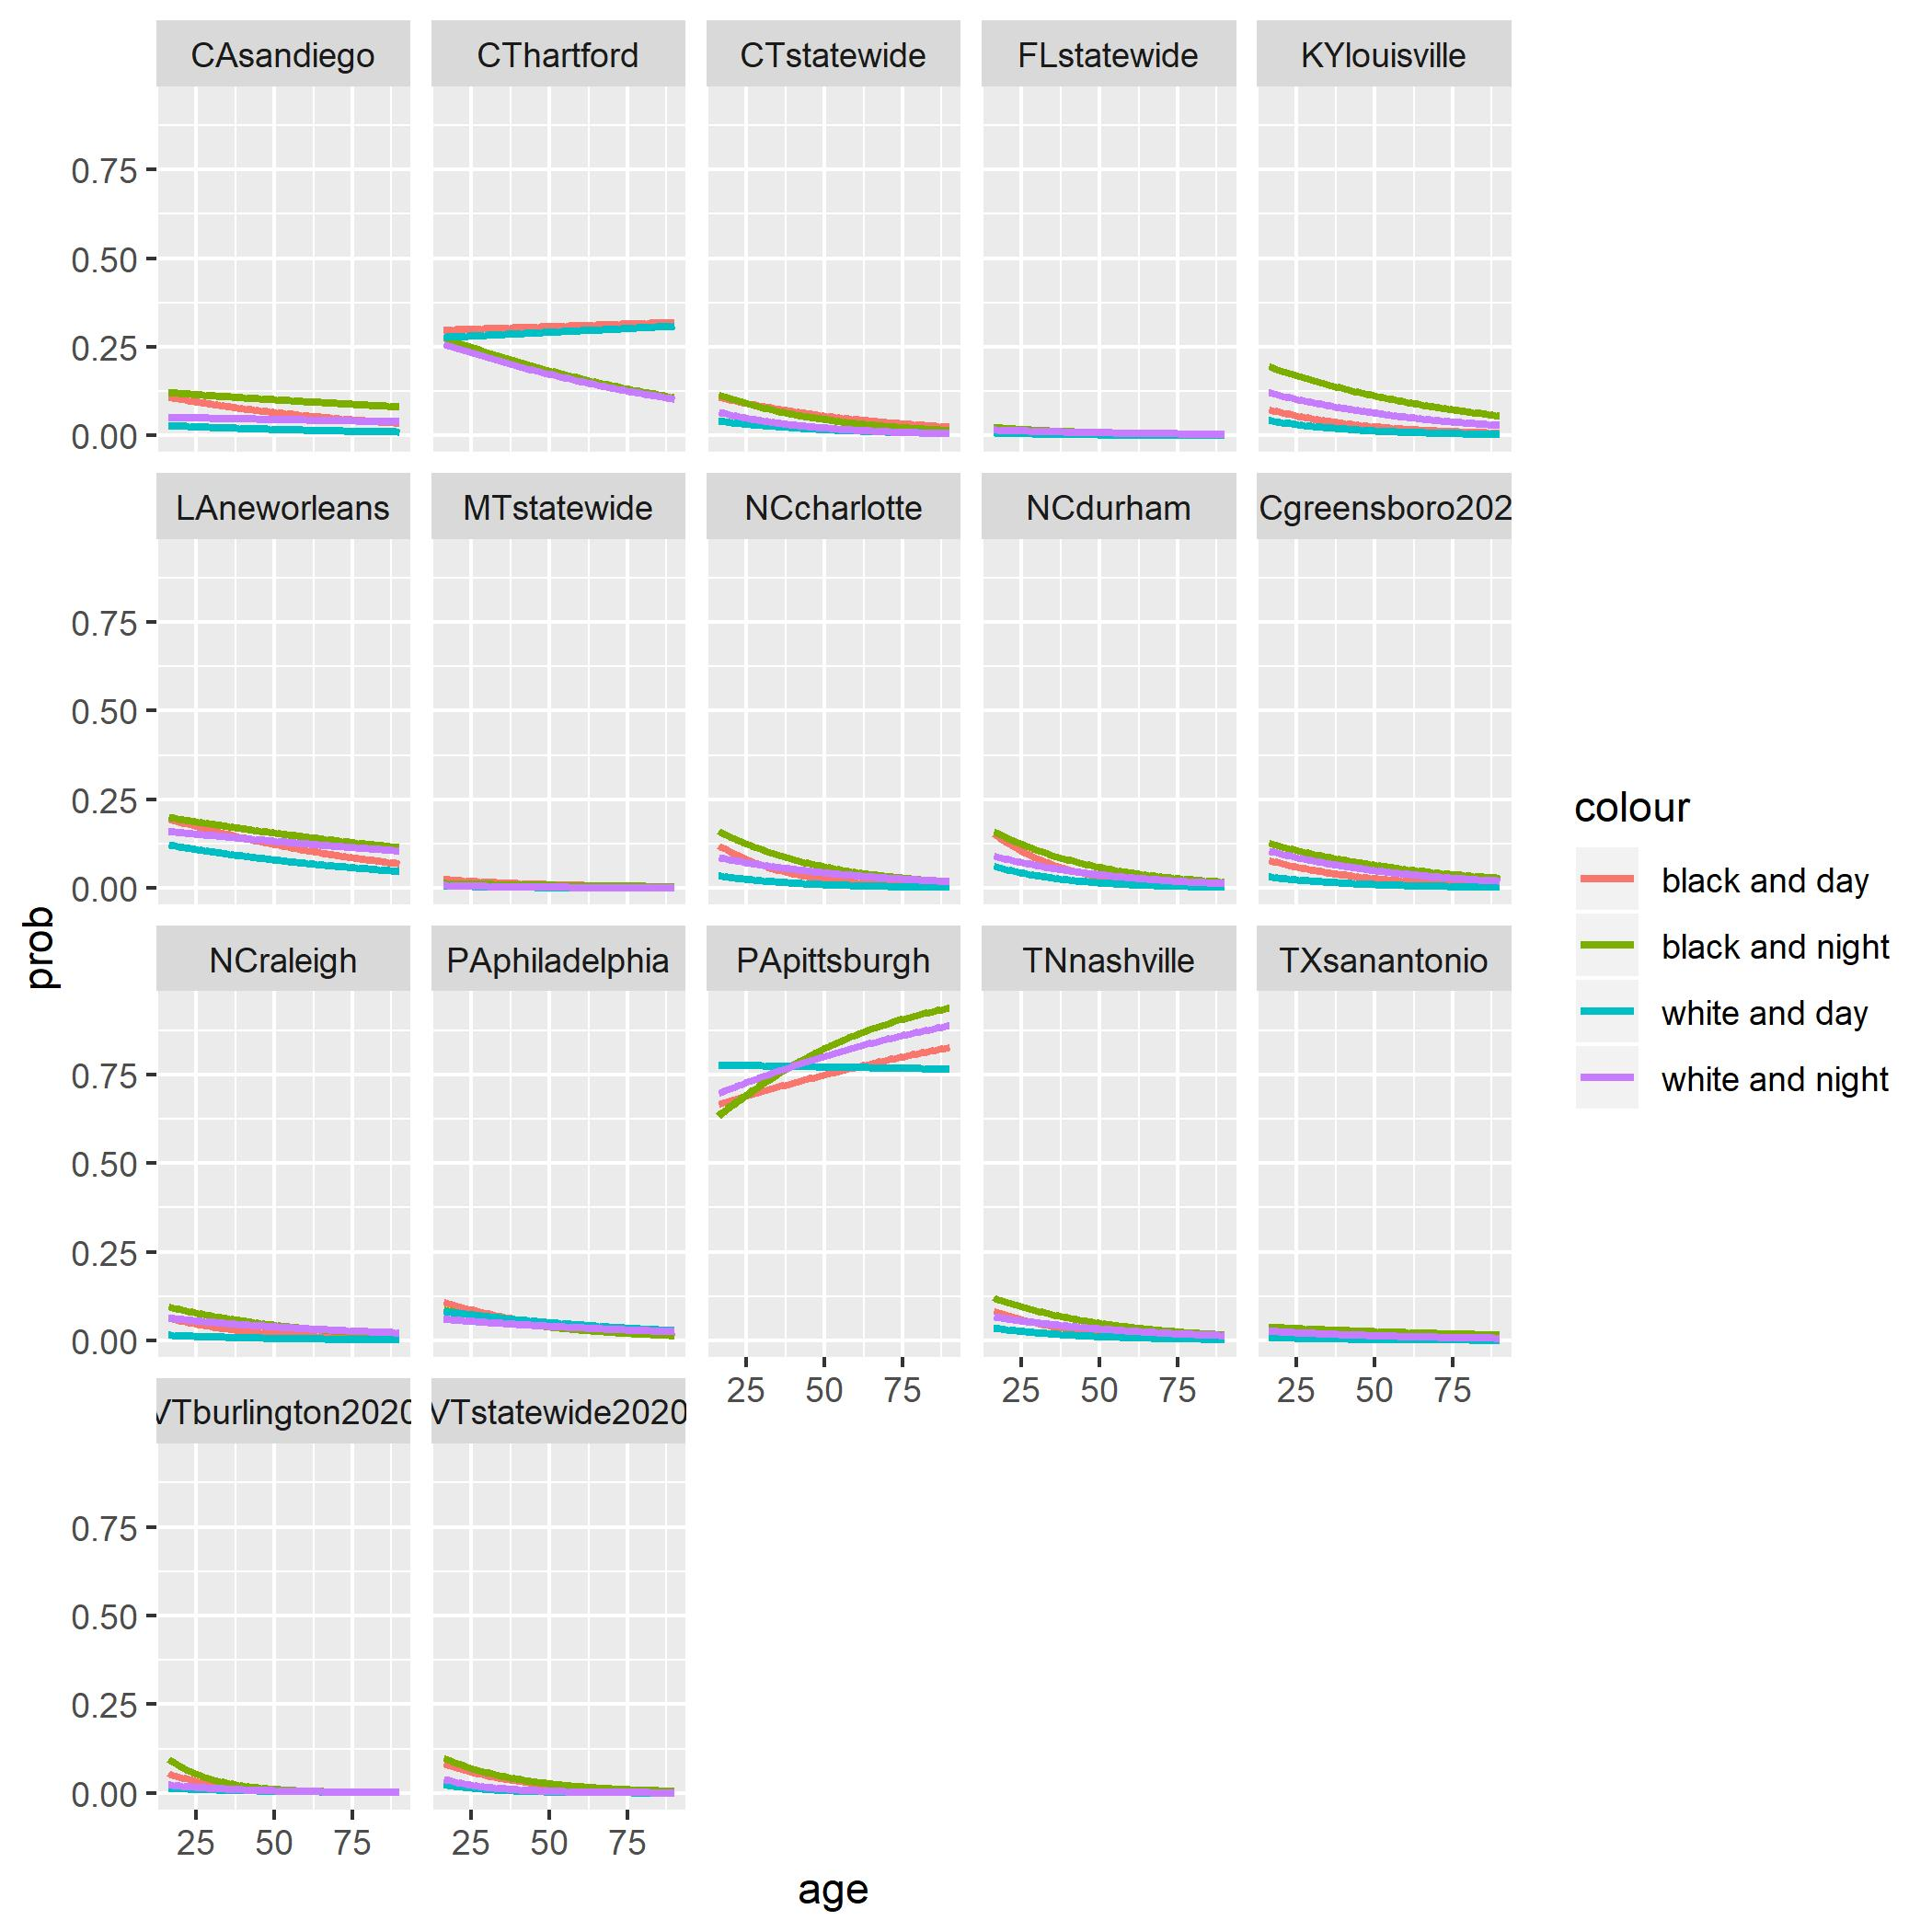
\includegraphics{cities_night_day_log_reg.jpg}

\hypertarget{final-words}{%
\chapter{Final Words}\label{final-words}}

We have finished a nice book.

  \bibliography{book.bib,packages.bib}

\end{document}
